% Generated by tools/build-figures.mjs.
% Source route_report: runs/m3-routes/report.json
% Source pipeline_report: runs/m3-compare/report.json
% Source coverage_report: runs/m3-coverage/report.json
% Include with % Generated by tools/build-figures.mjs.
% Source route_report: runs/m3-routes/report.json
% Source pipeline_report: runs/m3-compare/report.json
% Source coverage_report: runs/m3-coverage/report.json
% Include with % Generated by tools/build-figures.mjs.
% Source route_report: runs/m3-routes/report.json
% Source pipeline_report: runs/m3-compare/report.json
% Source coverage_report: runs/m3-coverage/report.json
% Include with % Generated by tools/build-figures.mjs.
% Source route_report: runs/m3-routes/report.json
% Source pipeline_report: runs/m3-compare/report.json
% Source coverage_report: runs/m3-coverage/report.json
% Include with \input{figures/manuscript/figures.tex} or copy individual figure blocks.

\begin{figure}[t]
  \centering
  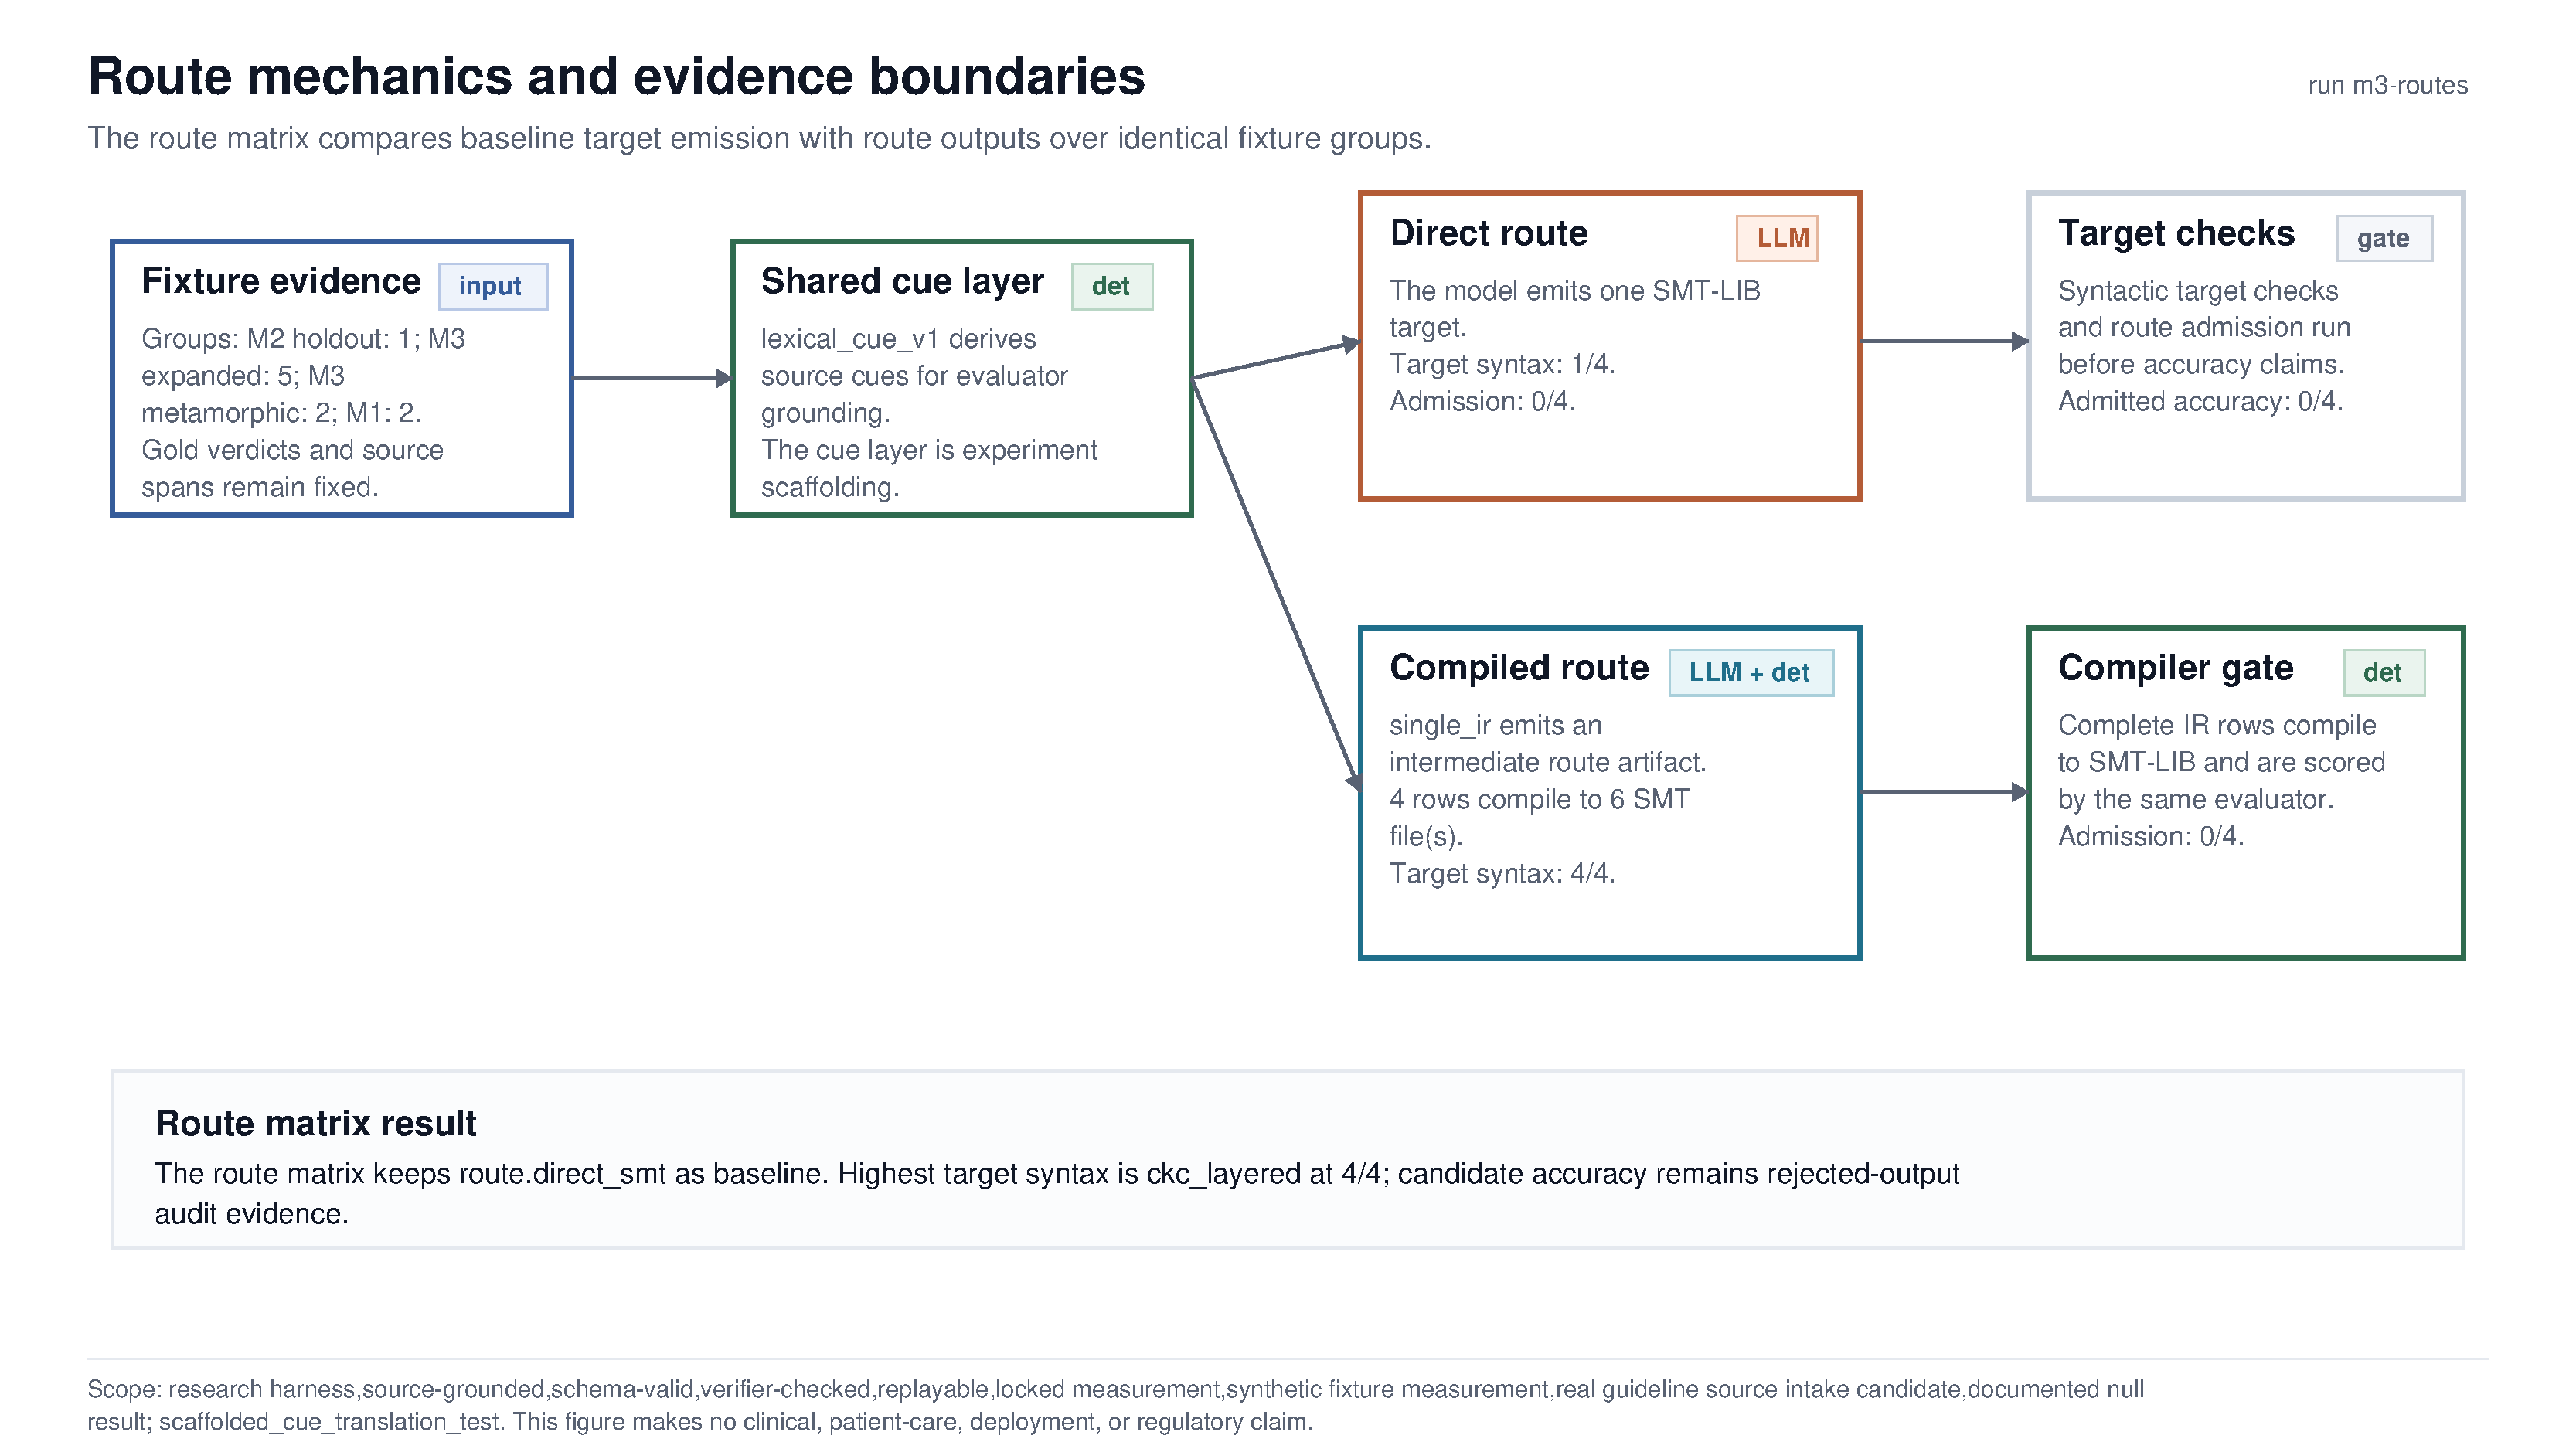
\includegraphics[width=\linewidth]{figures/manuscript/fig01_route_mechanics.pdf}
  \caption{Route mechanics. Implemented routes consume the same fixture groups and are scored by the same evaluator; the current run shows a target-syntax baseline delta only, not an admitted-verdict baseline delta.}
  \label{fig:route-mechanics}
\end{figure}

\begin{figure}[t]
  \centering
  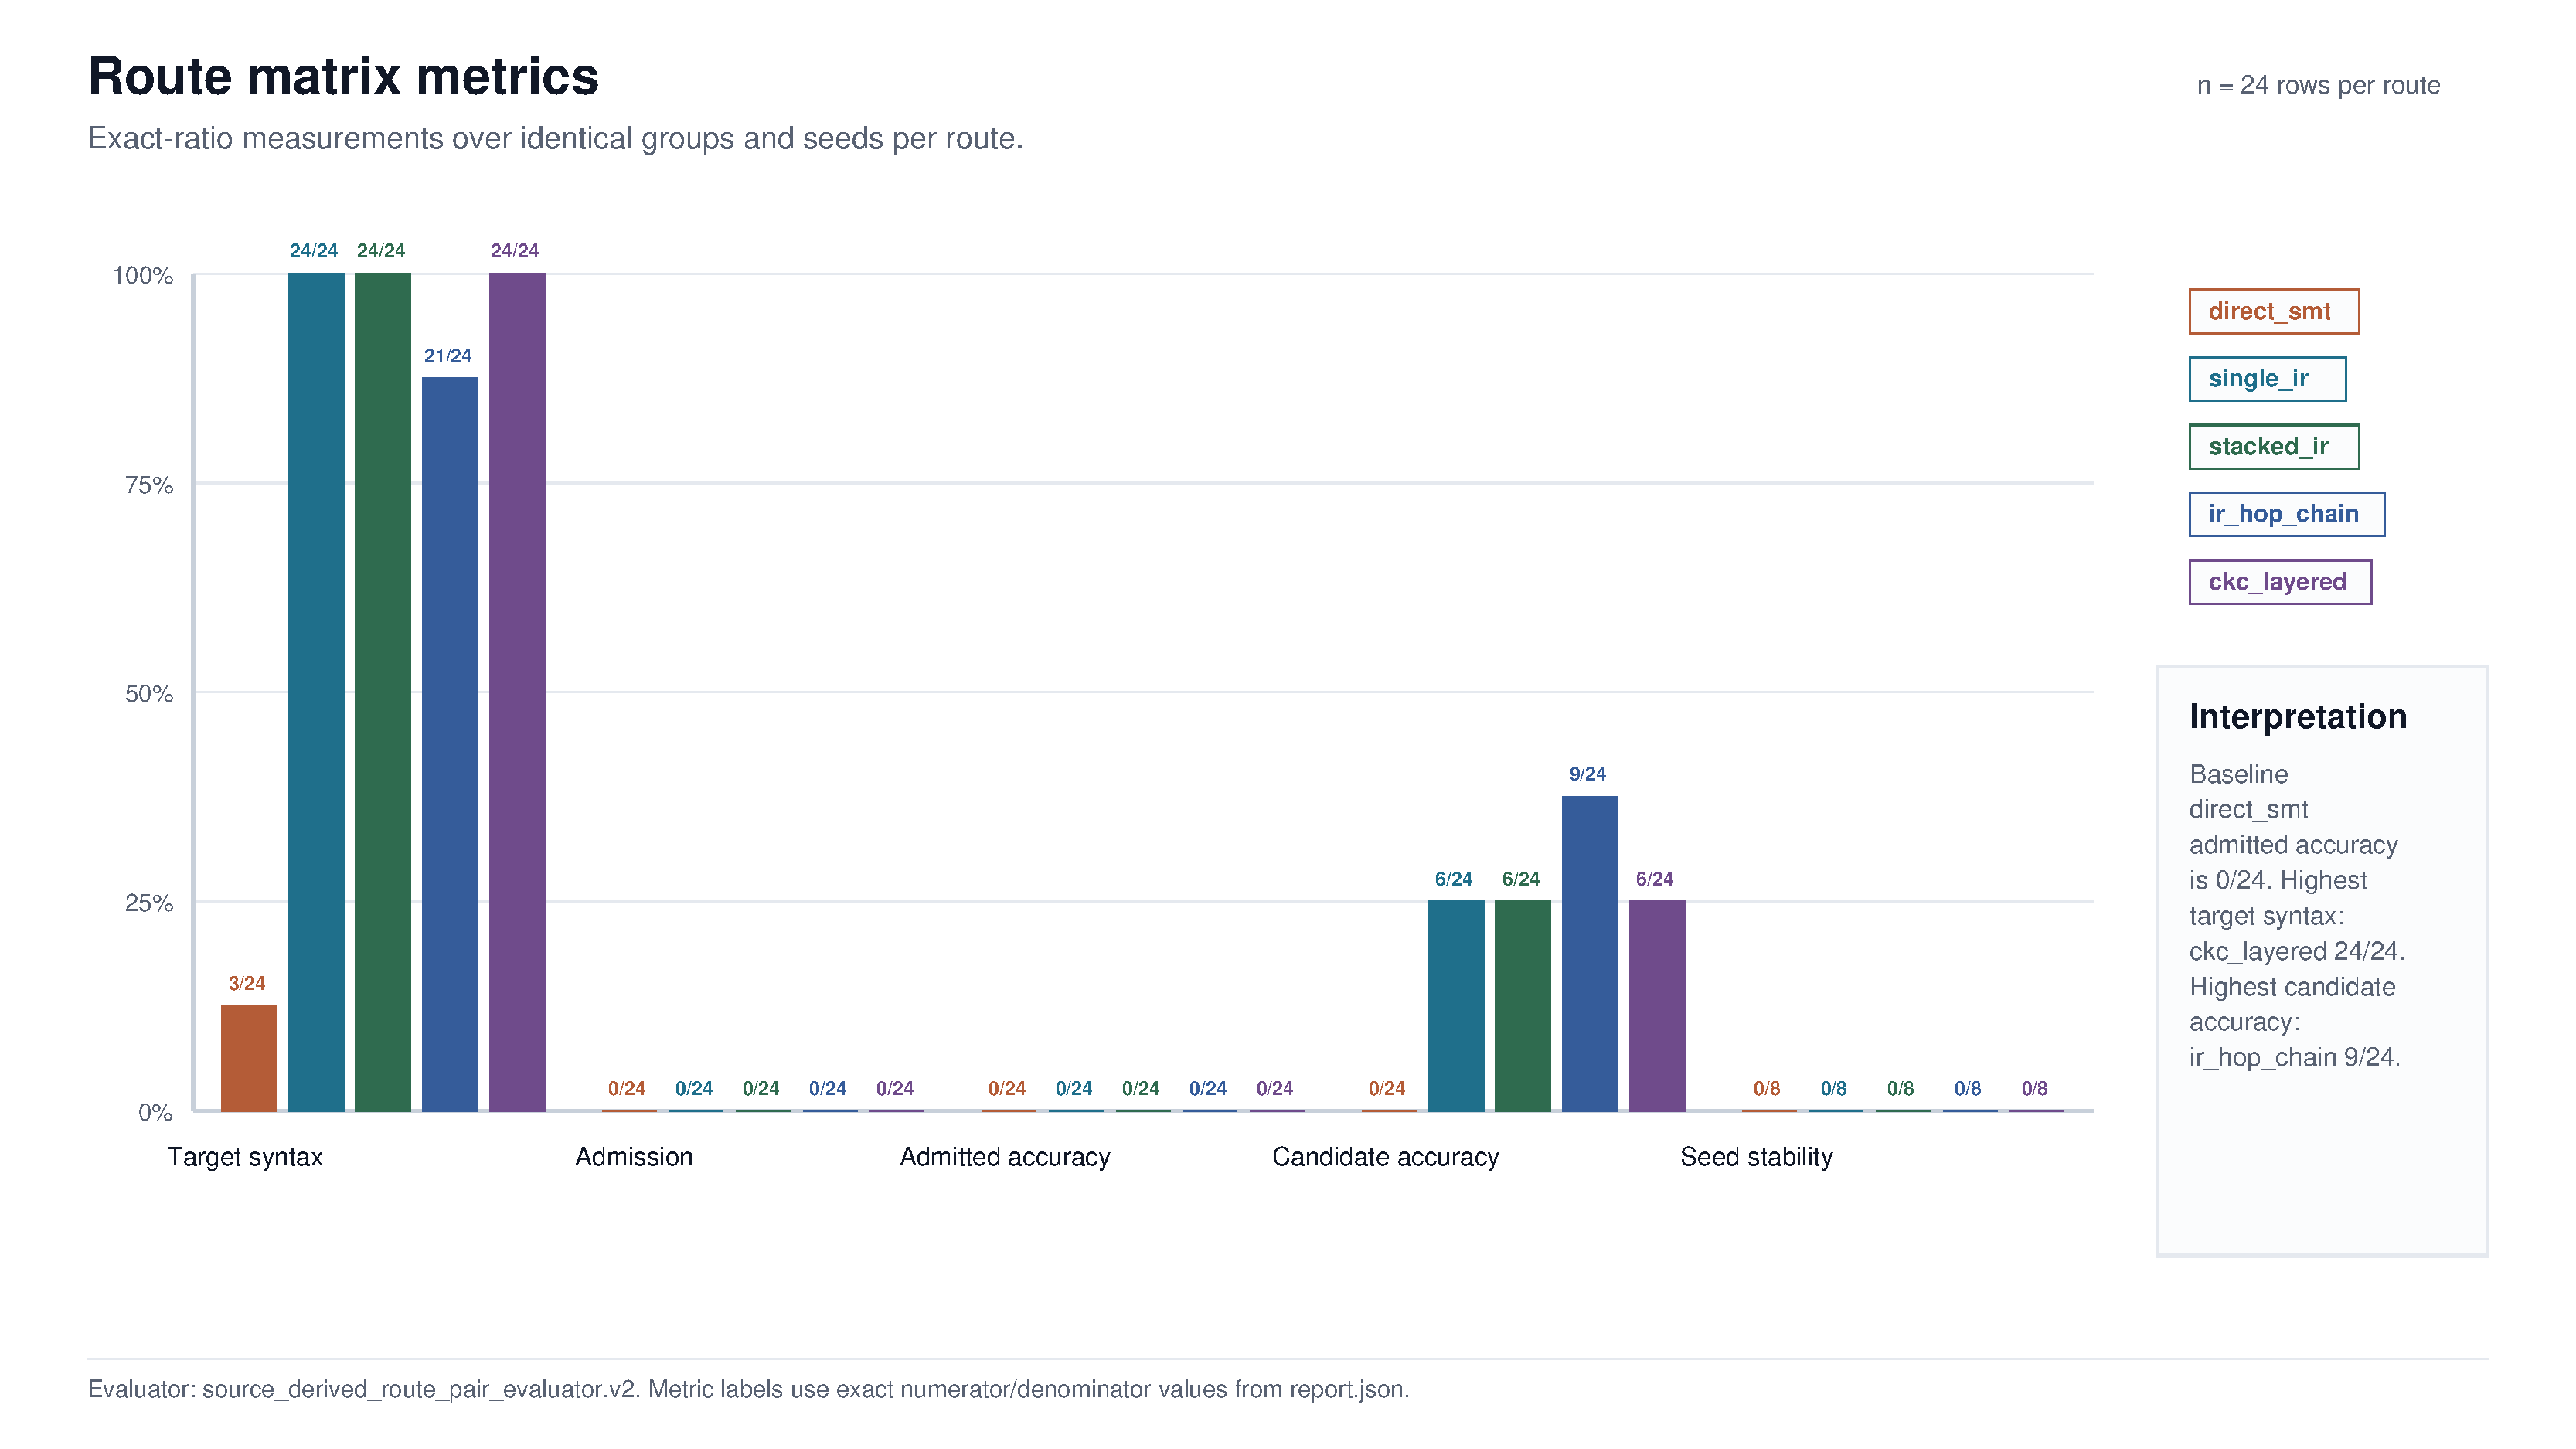
\includegraphics[width=\linewidth]{figures/manuscript/fig02_route_metrics.pdf}
  \caption{Route metrics from the current run, shown as exact-ratio profile lines over the route matrix with direct SMT retained as baseline. Candidate verdict accuracy is rejected-output audit evidence, not admitted baseline improvement.}
  \label{fig:route-metrics}
\end{figure}

\begin{figure}[t]
  \centering
  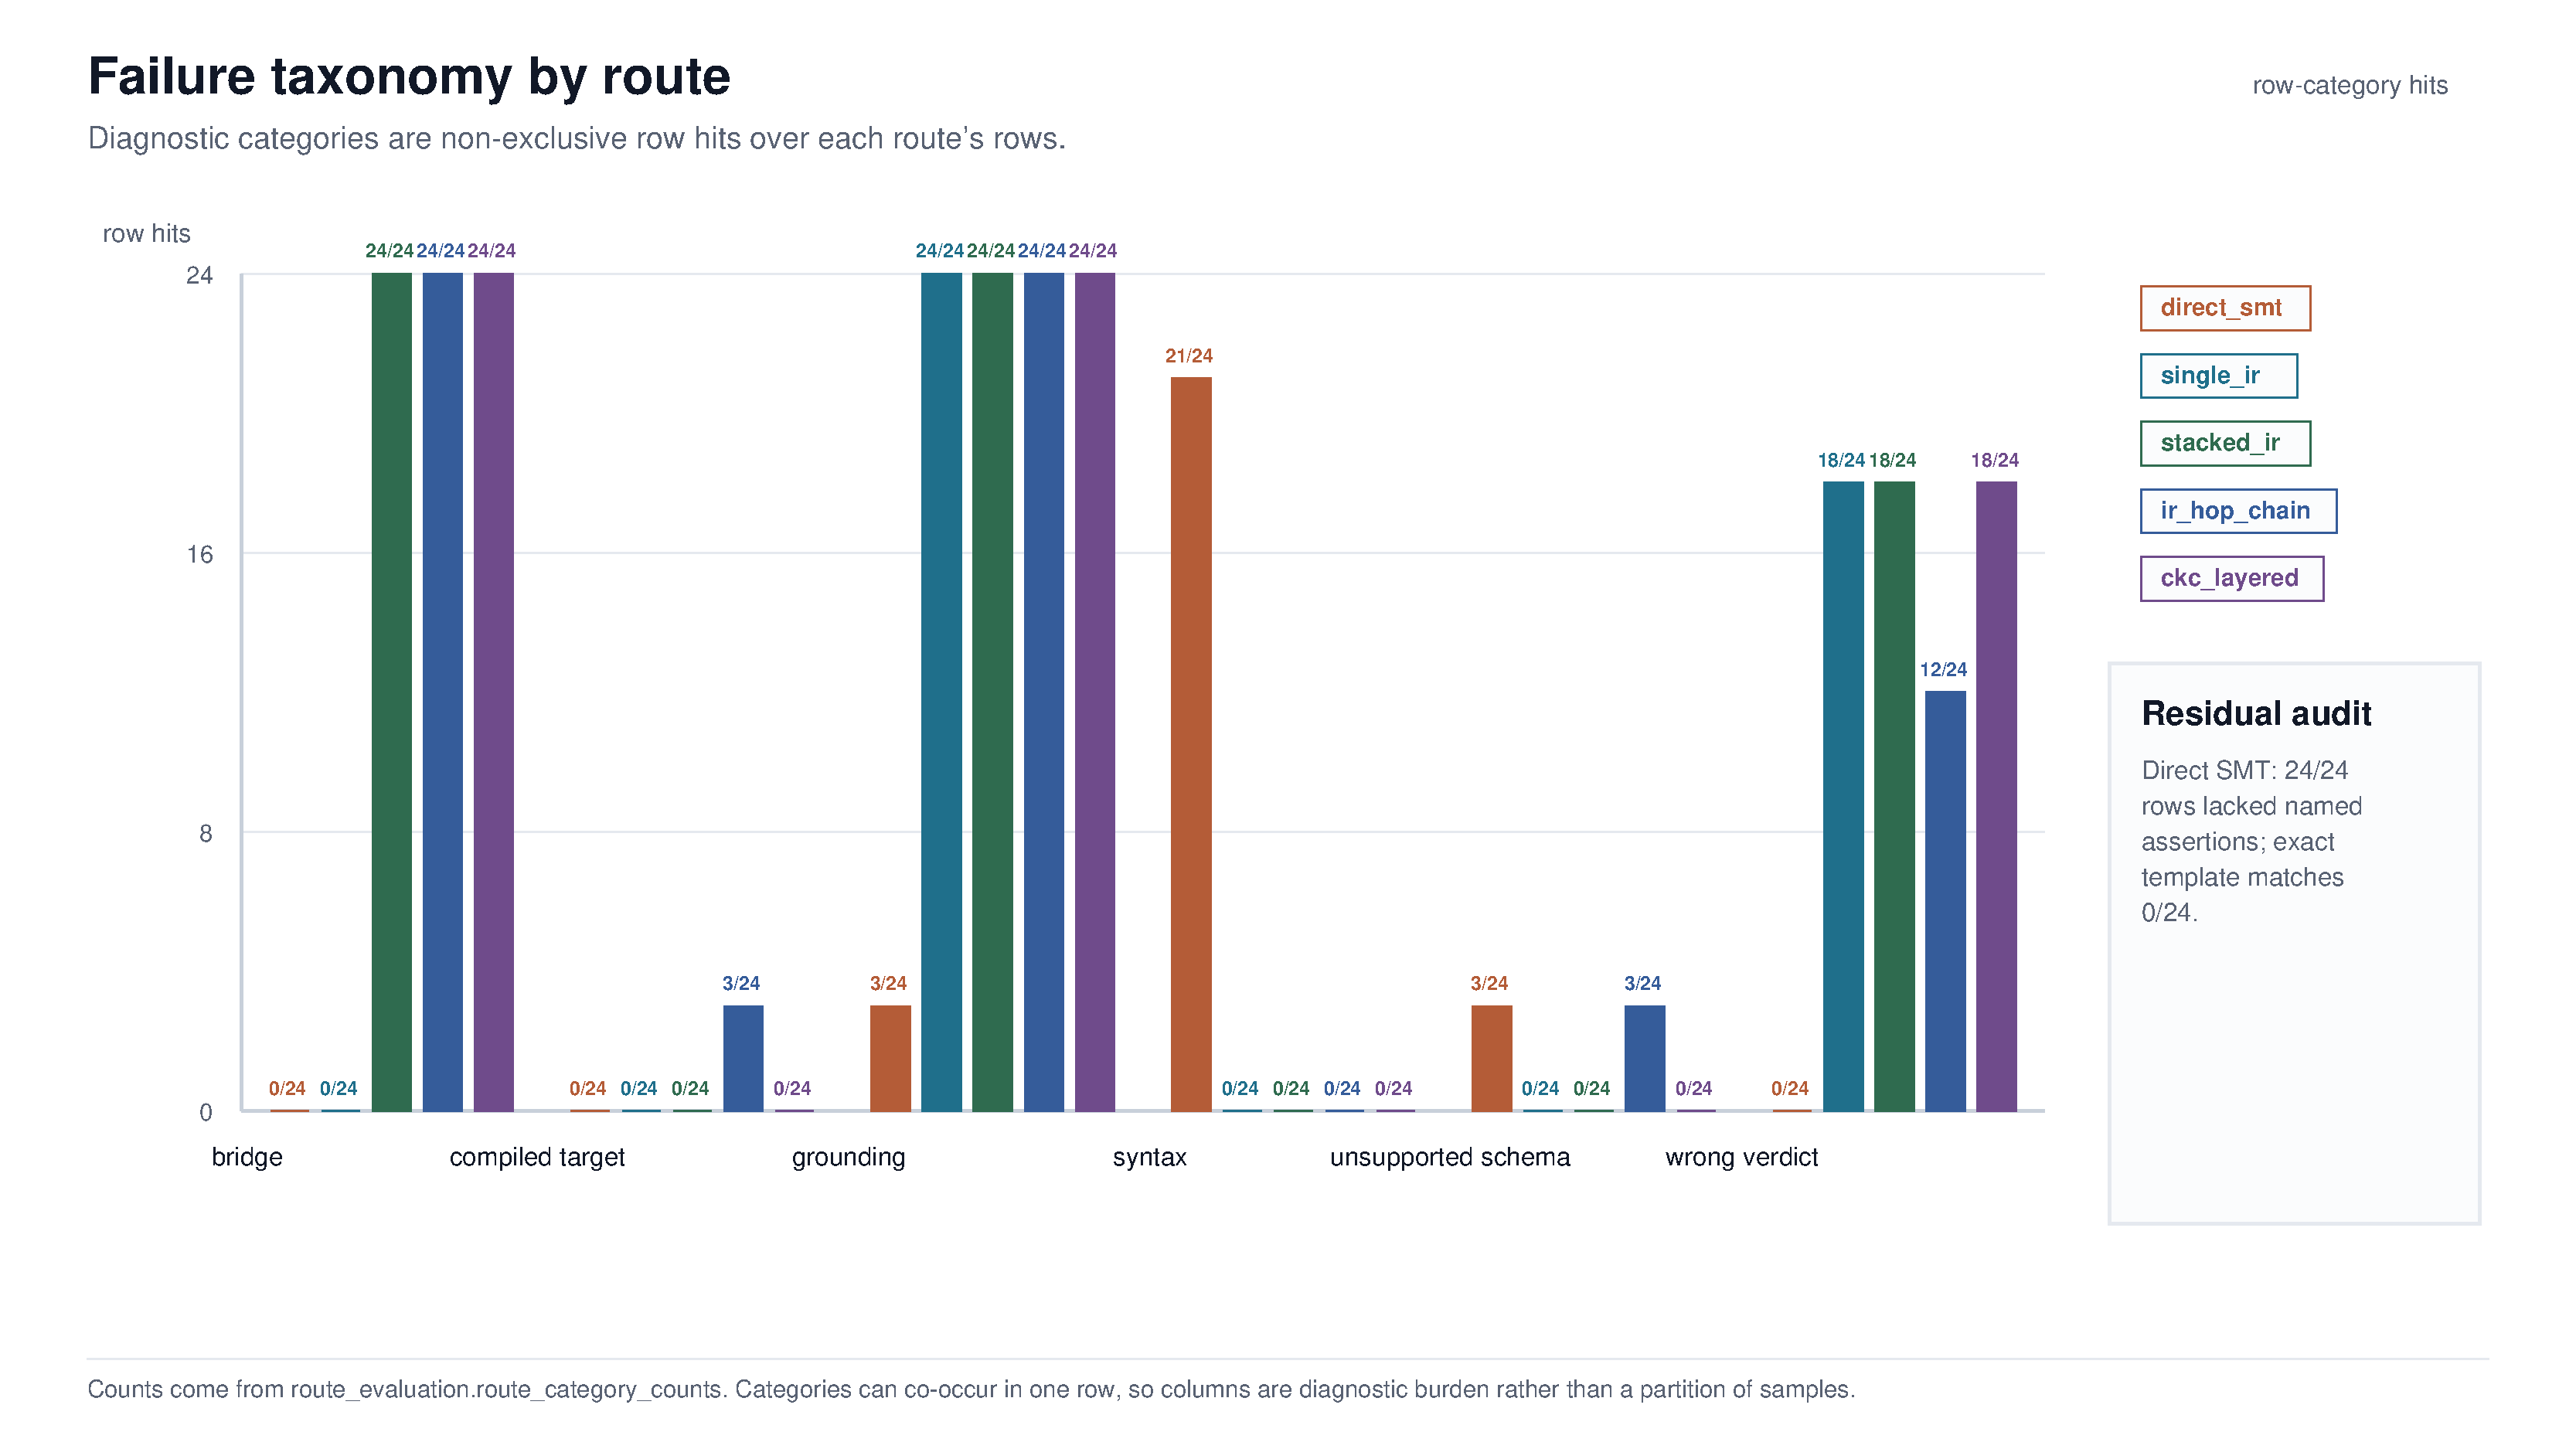
\includegraphics[width=\linewidth]{figures/manuscript/fig03_failure_taxonomy.pdf}
  \caption{Diagnostic row-category hits are shown as route profiles over the route matrix. Categories can co-occur, so profiles show diagnostic burden rather than a partition of samples.}
  \label{fig:failure-taxonomy}
\end{figure}

\begin{figure}[t]
  \centering
  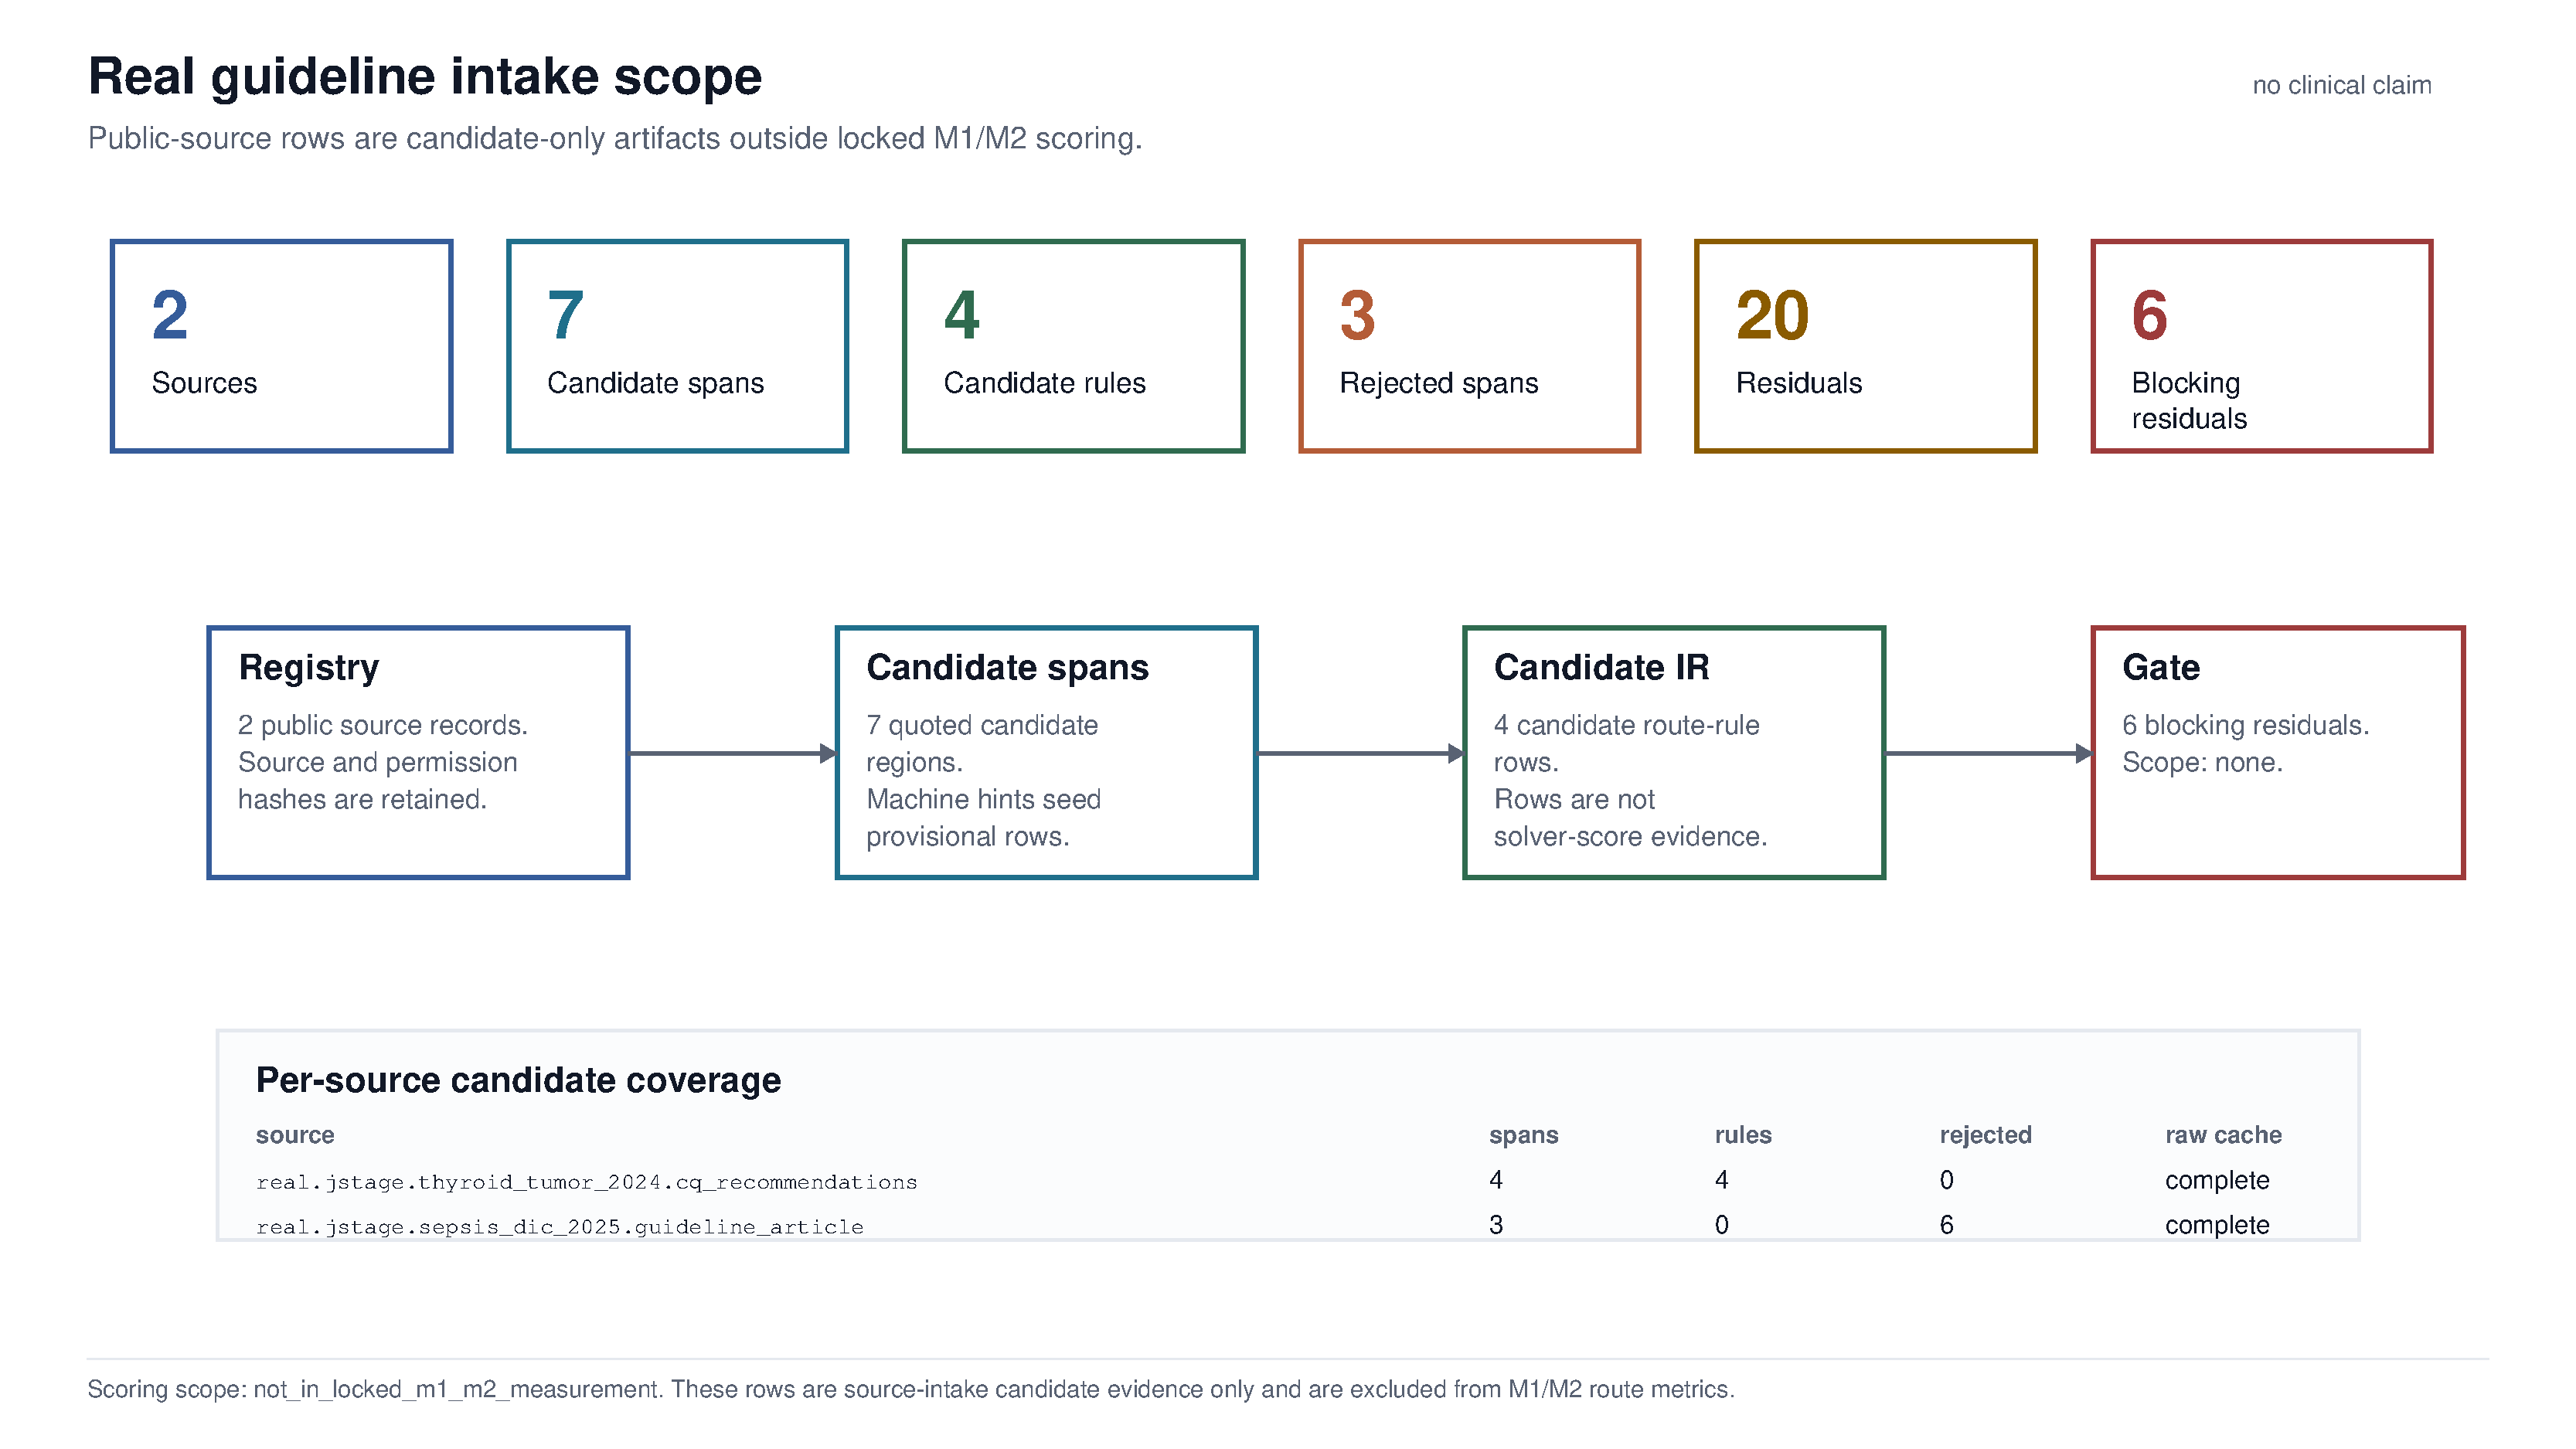
\includegraphics[width=\linewidth]{figures/manuscript/fig04_real_source_intake.pdf}
  \caption{Real Japanese guideline sources are represented as candidate-only source-intake artifacts with source and permission hashes, but they remain outside locked M1/M2 scoring and carry no clinical claim.}
  \label{fig:real-source-intake}
\end{figure}

\begin{figure}[t]
  \centering
  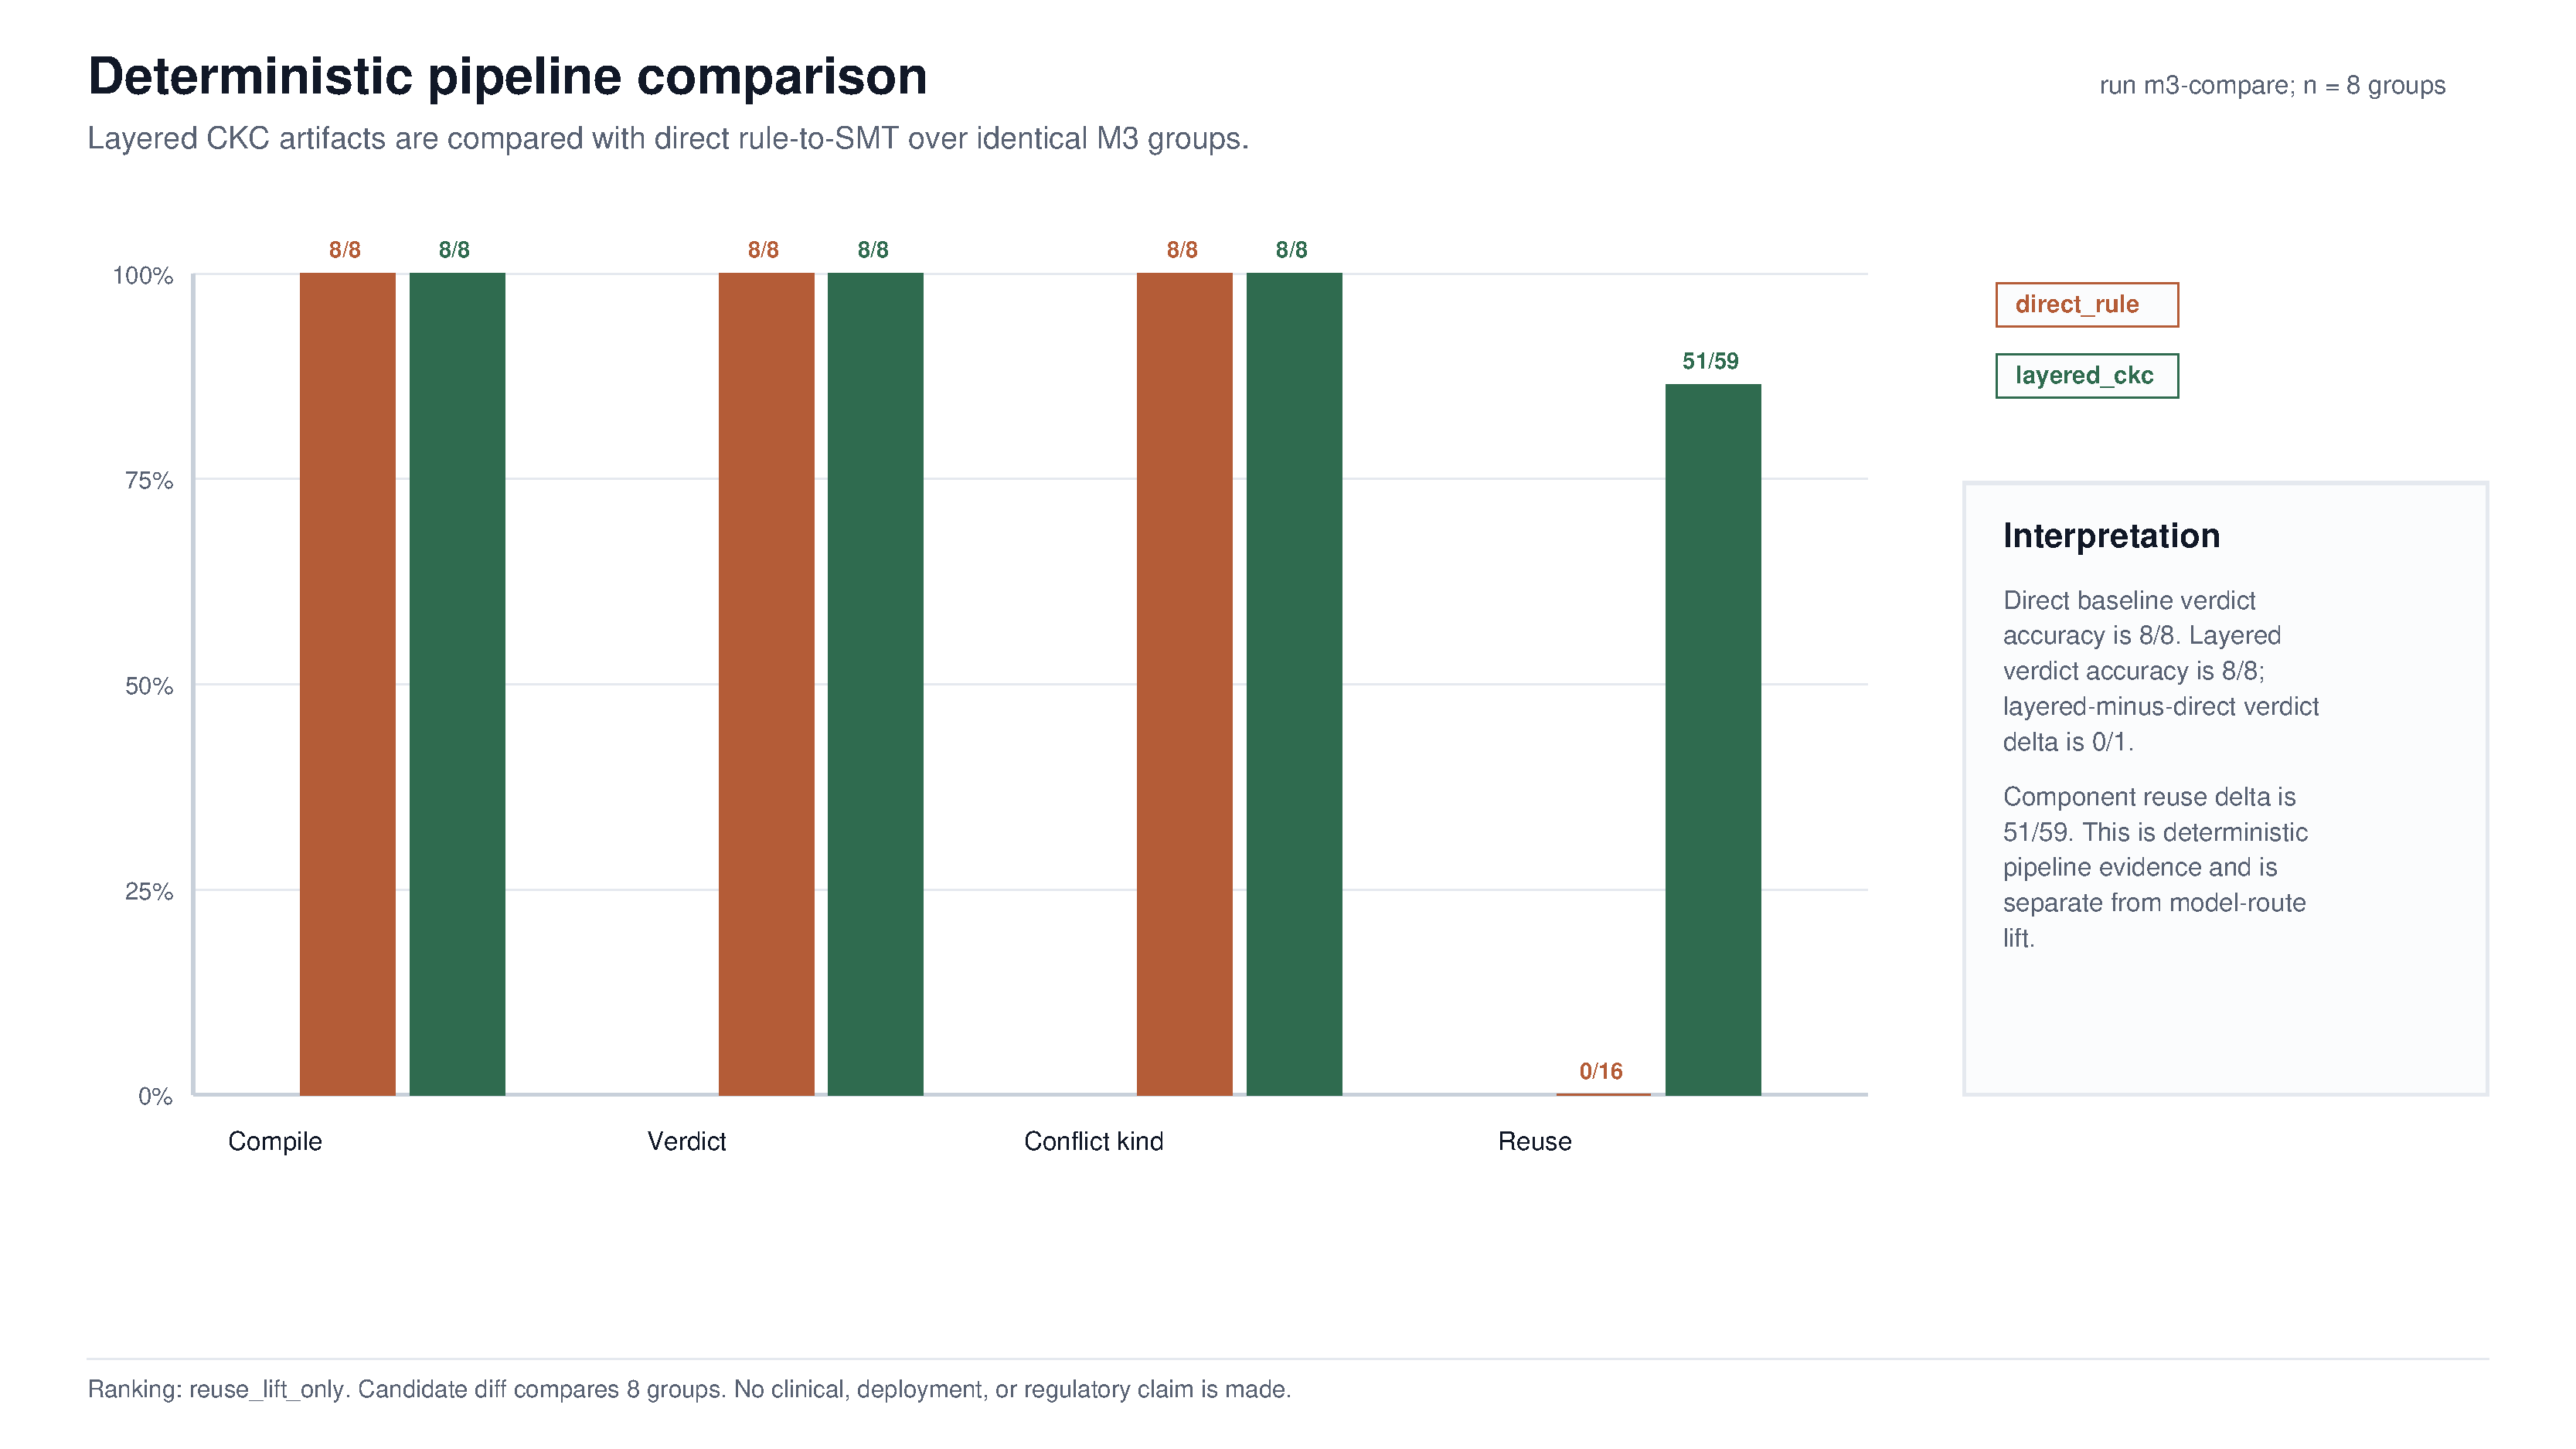
\includegraphics[width=\linewidth]{figures/manuscript/fig05_pipeline_comparison.pdf}
  \caption{Deterministic pipeline comparison. Direct rule-to-SMT is retained as baseline; profile lines show that the layered CKC pipeline matches verdict and conflict-kind accuracy in the current M3 comparison while component reuse is reported separately from model-route baseline deltas.}
  \label{fig:pipeline-comparison}
\end{figure}

\begin{figure}[t]
  \centering
  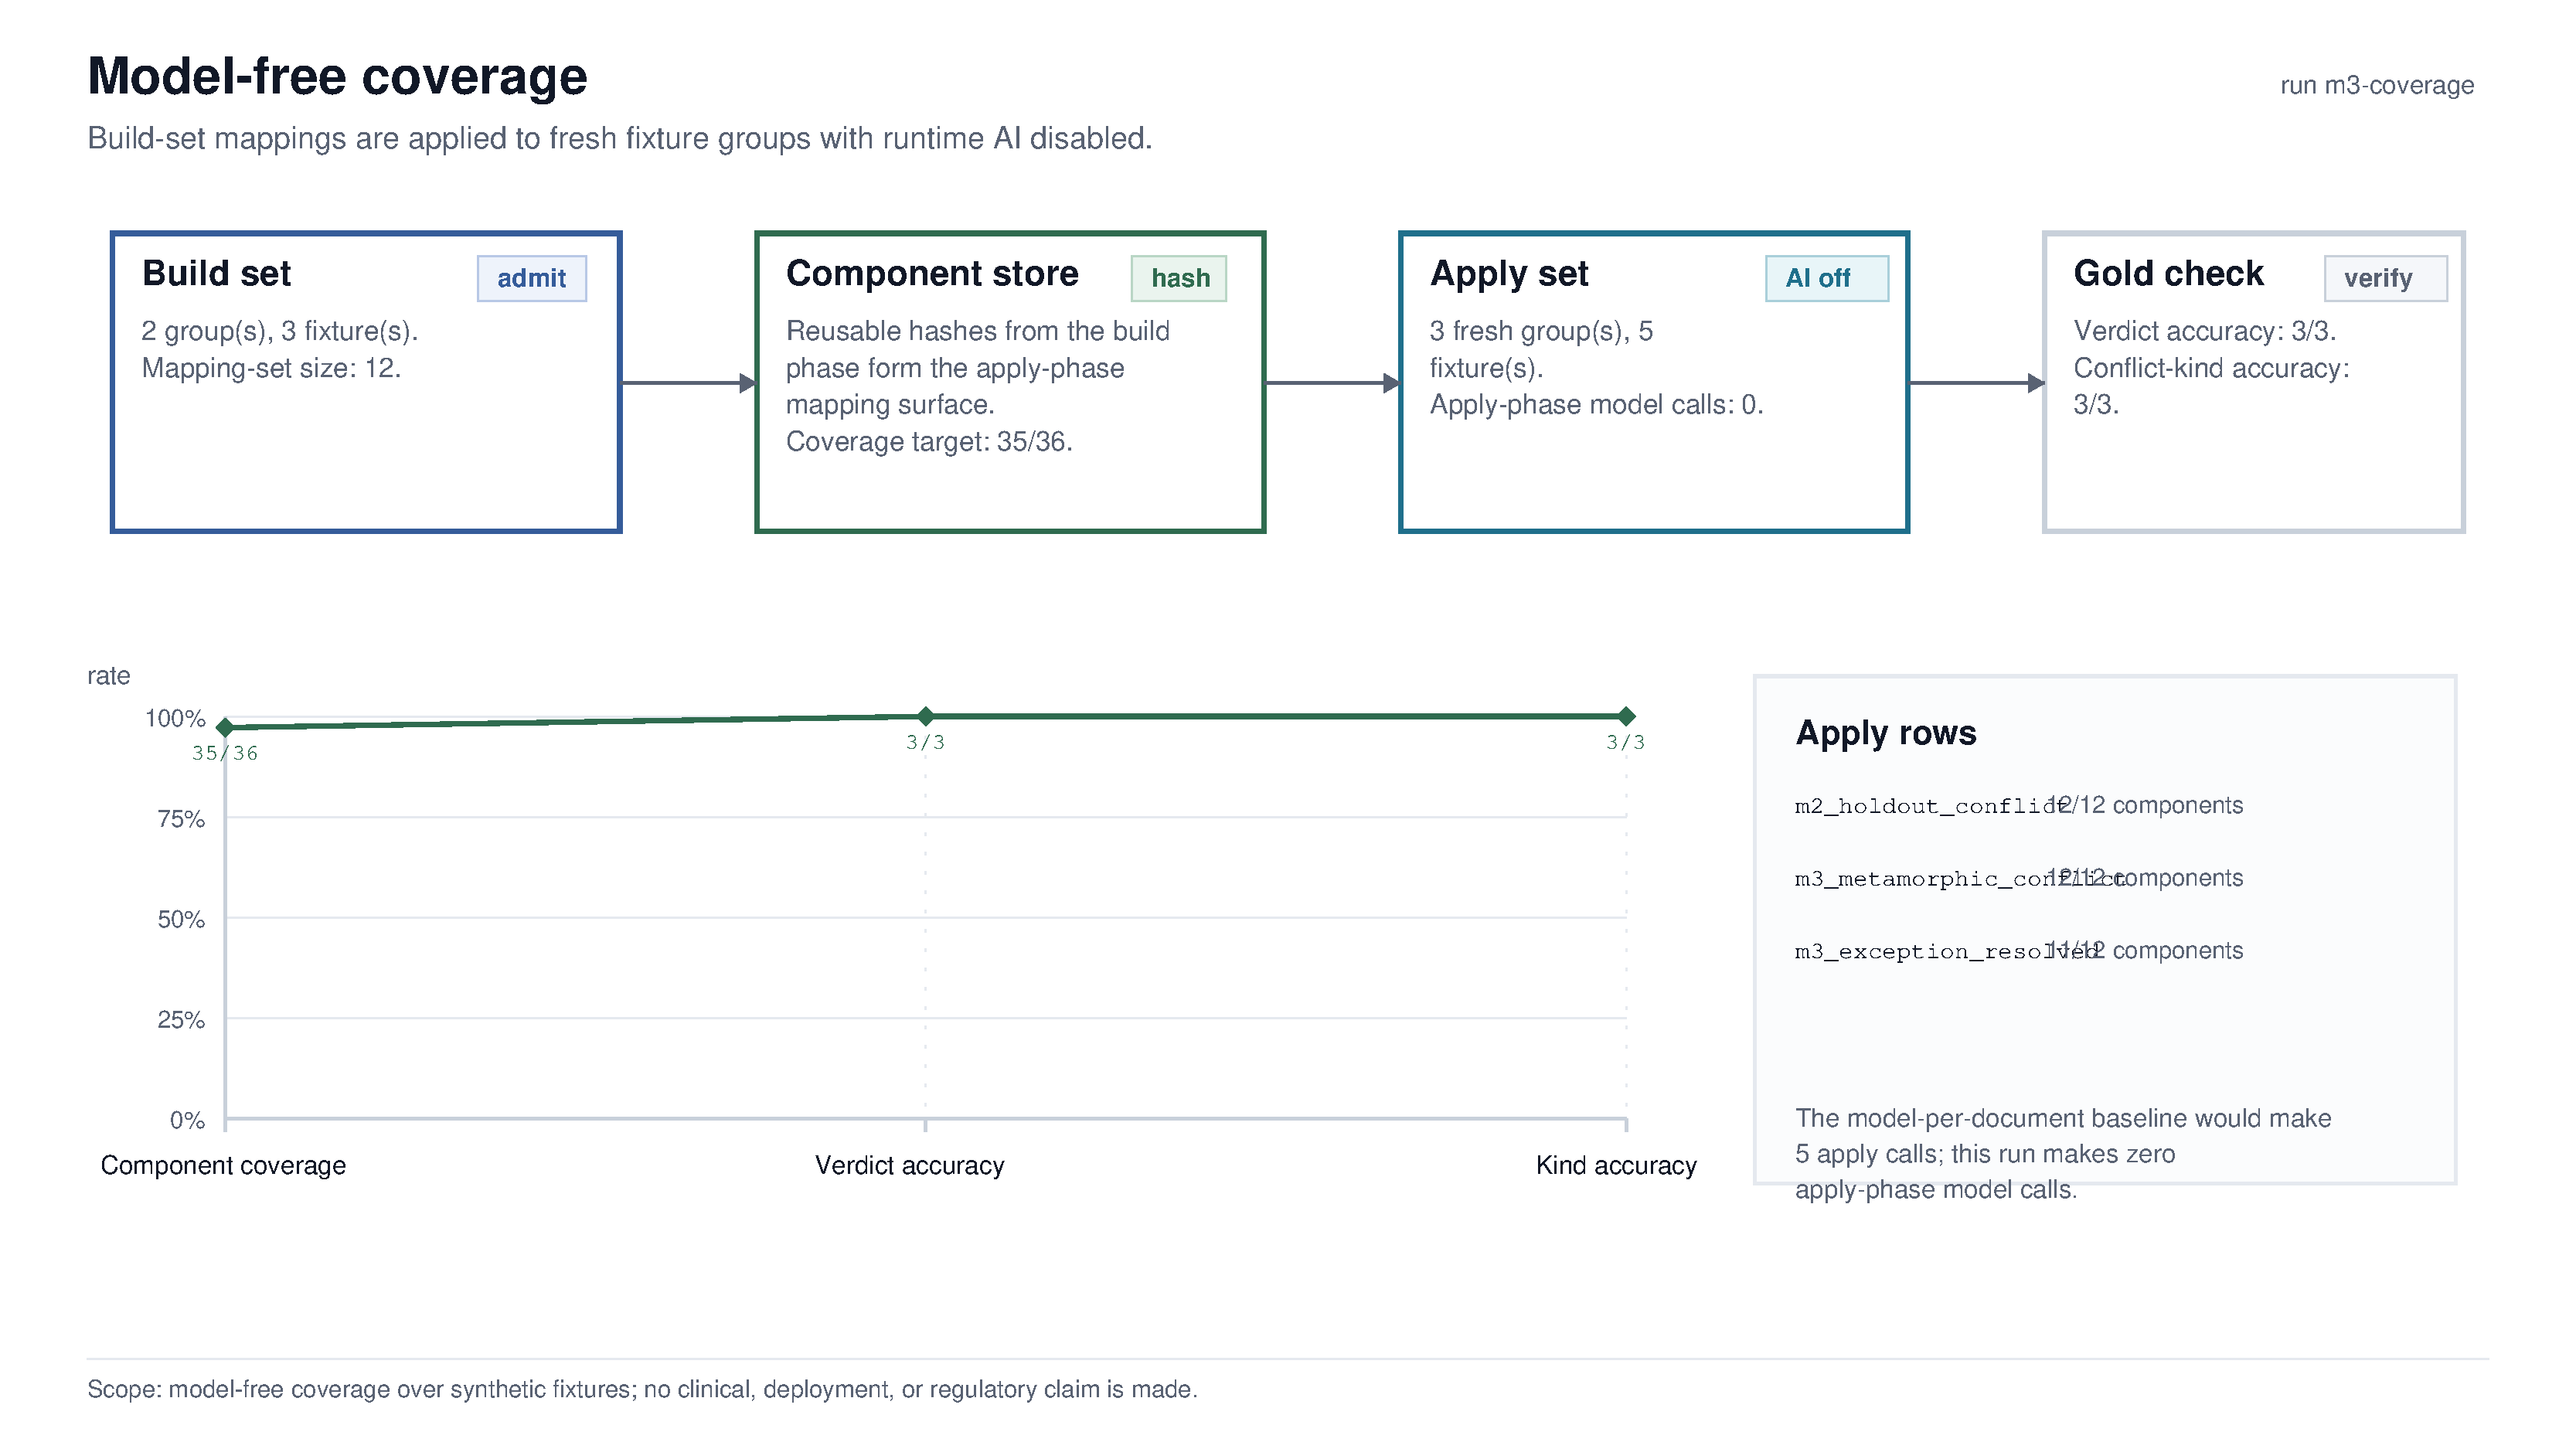
\includegraphics[width=\linewidth]{figures/manuscript/fig06_model_free_coverage.pdf}
  \caption{Model-free coverage. Build-set mappings are applied to fresh synthetic fixture groups with runtime AI disabled; component coverage, verdict accuracy, and zero apply-phase model calls are reported as exact ratios/counts.}
  \label{fig:model-free-coverage}
\end{figure}
 or copy individual figure blocks.

\begin{figure}[t]
  \centering
  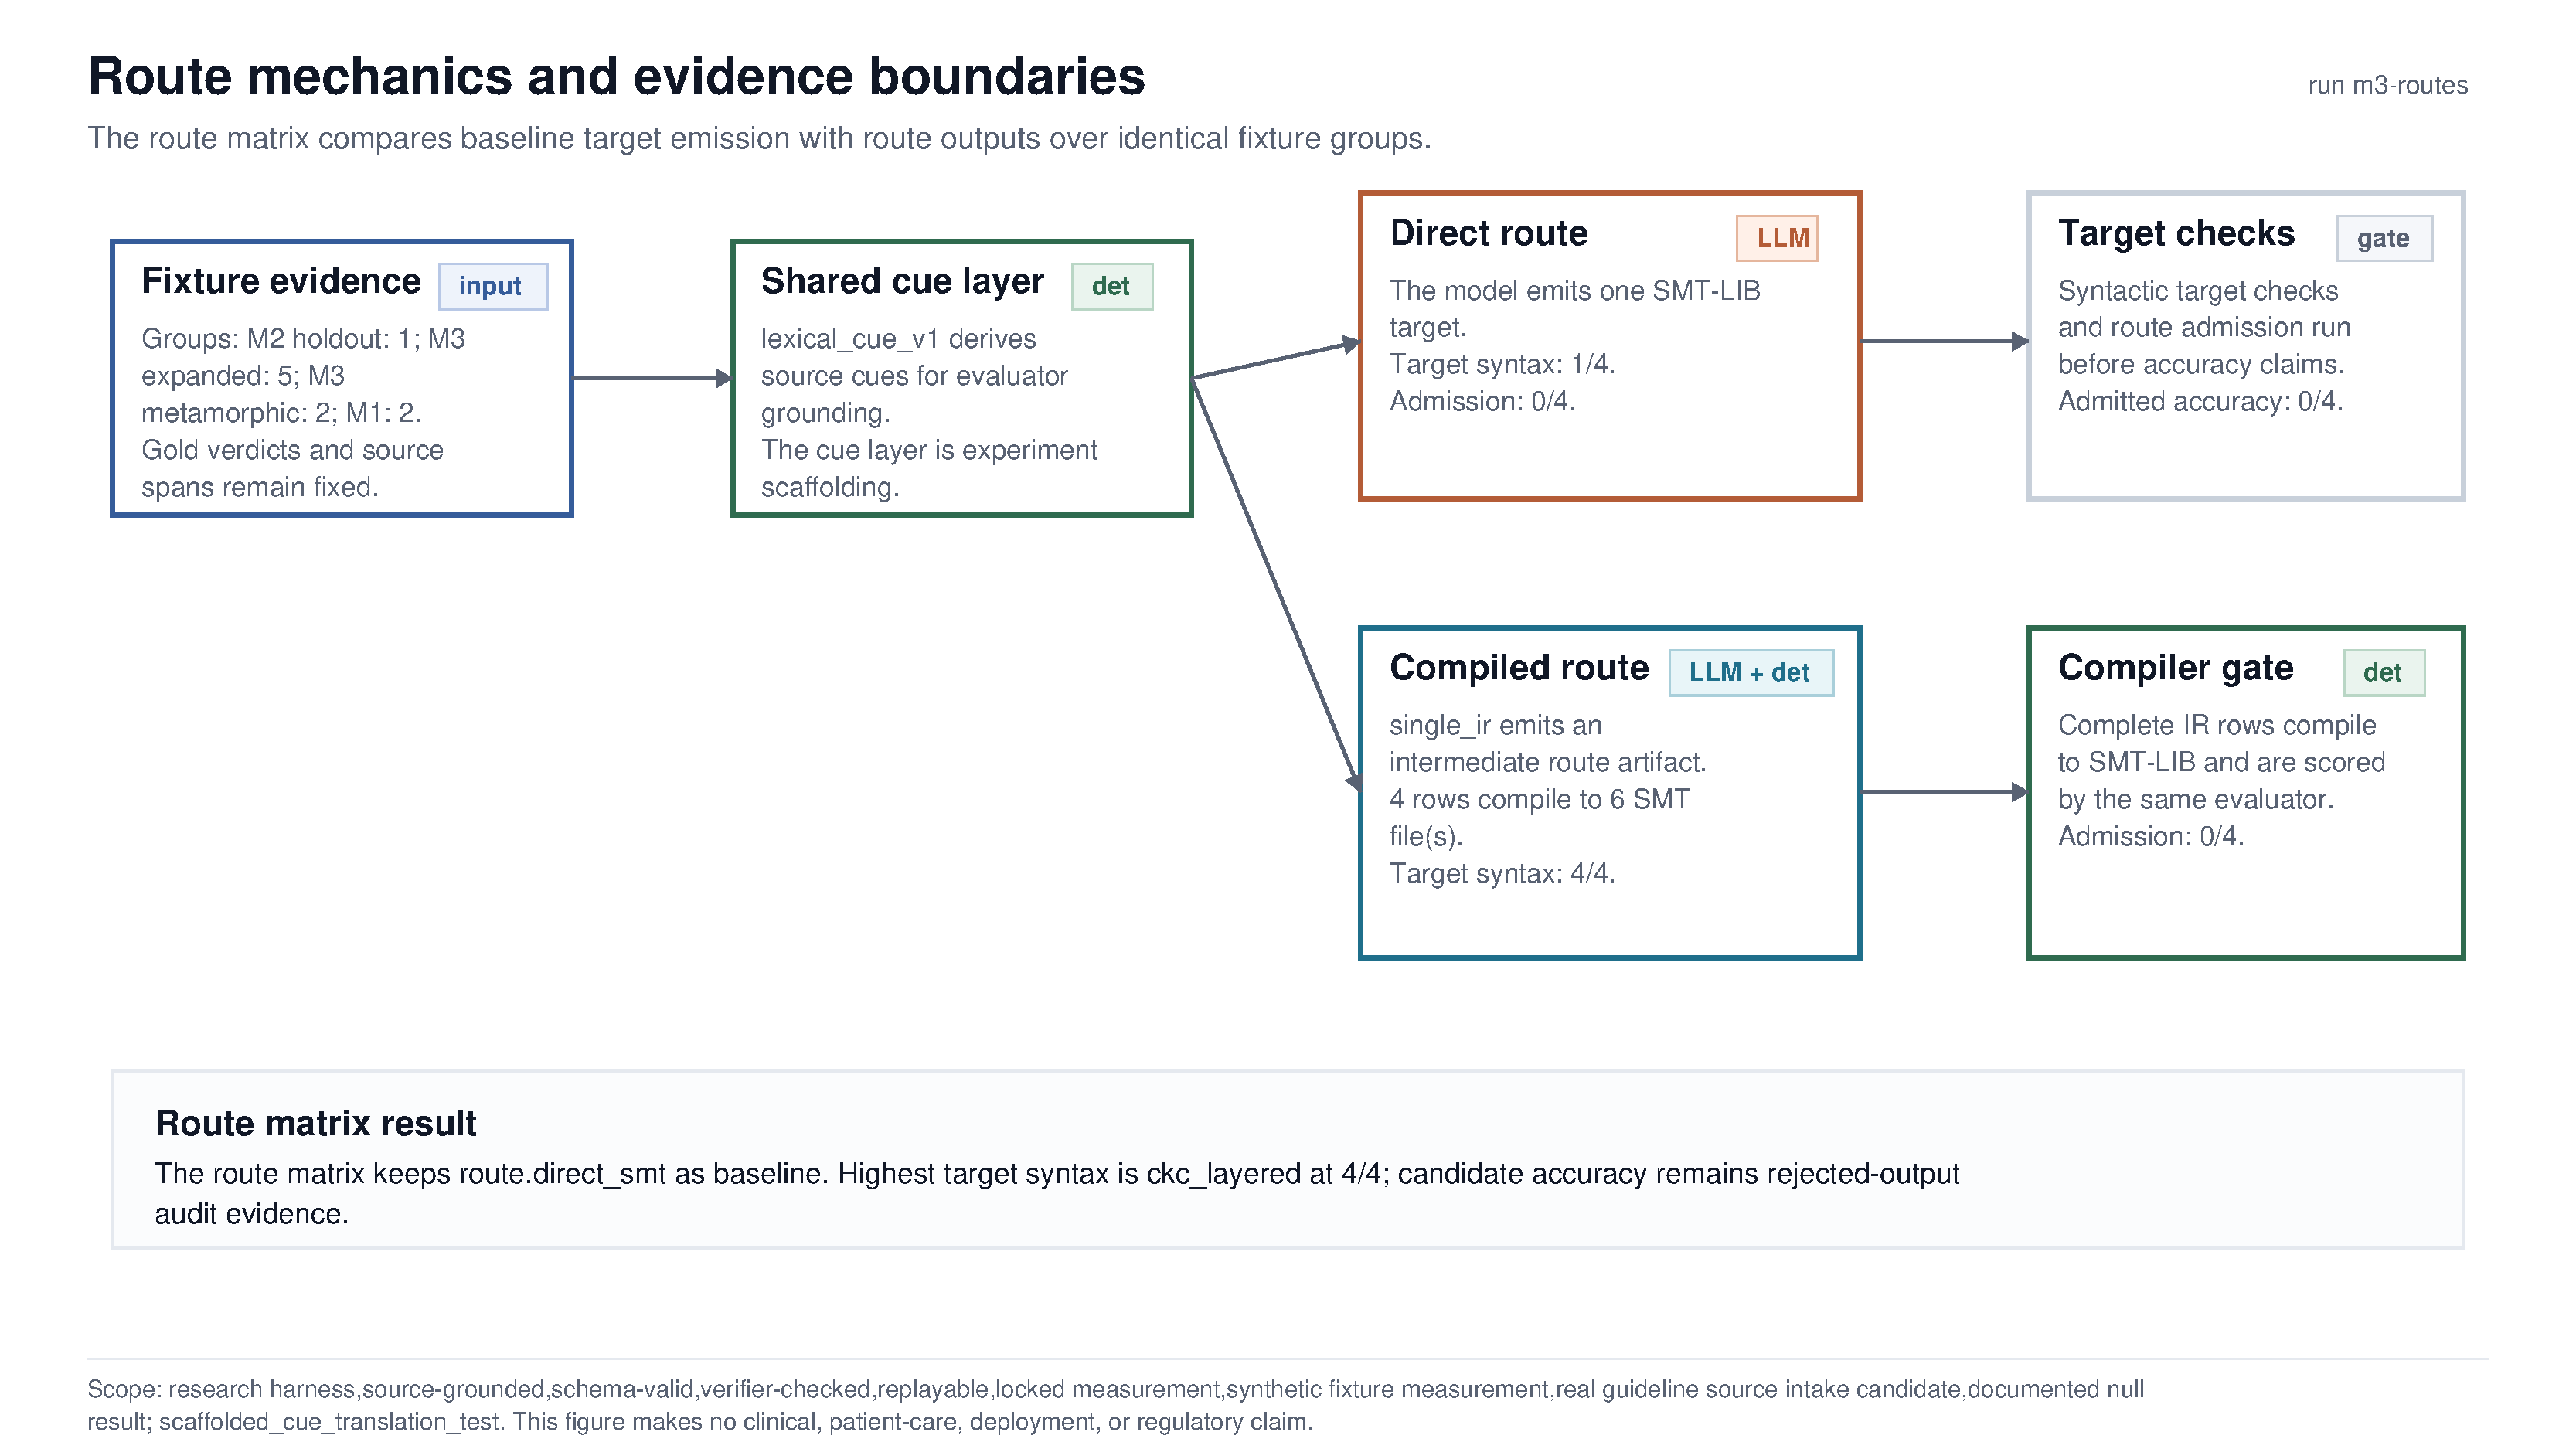
\includegraphics[width=\linewidth]{figures/manuscript/fig01_route_mechanics.pdf}
  \caption{Route mechanics. Implemented routes consume the same fixture groups and are scored by the same evaluator; the current run shows a target-syntax baseline delta only, not an admitted-verdict baseline delta.}
  \label{fig:route-mechanics}
\end{figure}

\begin{figure}[t]
  \centering
  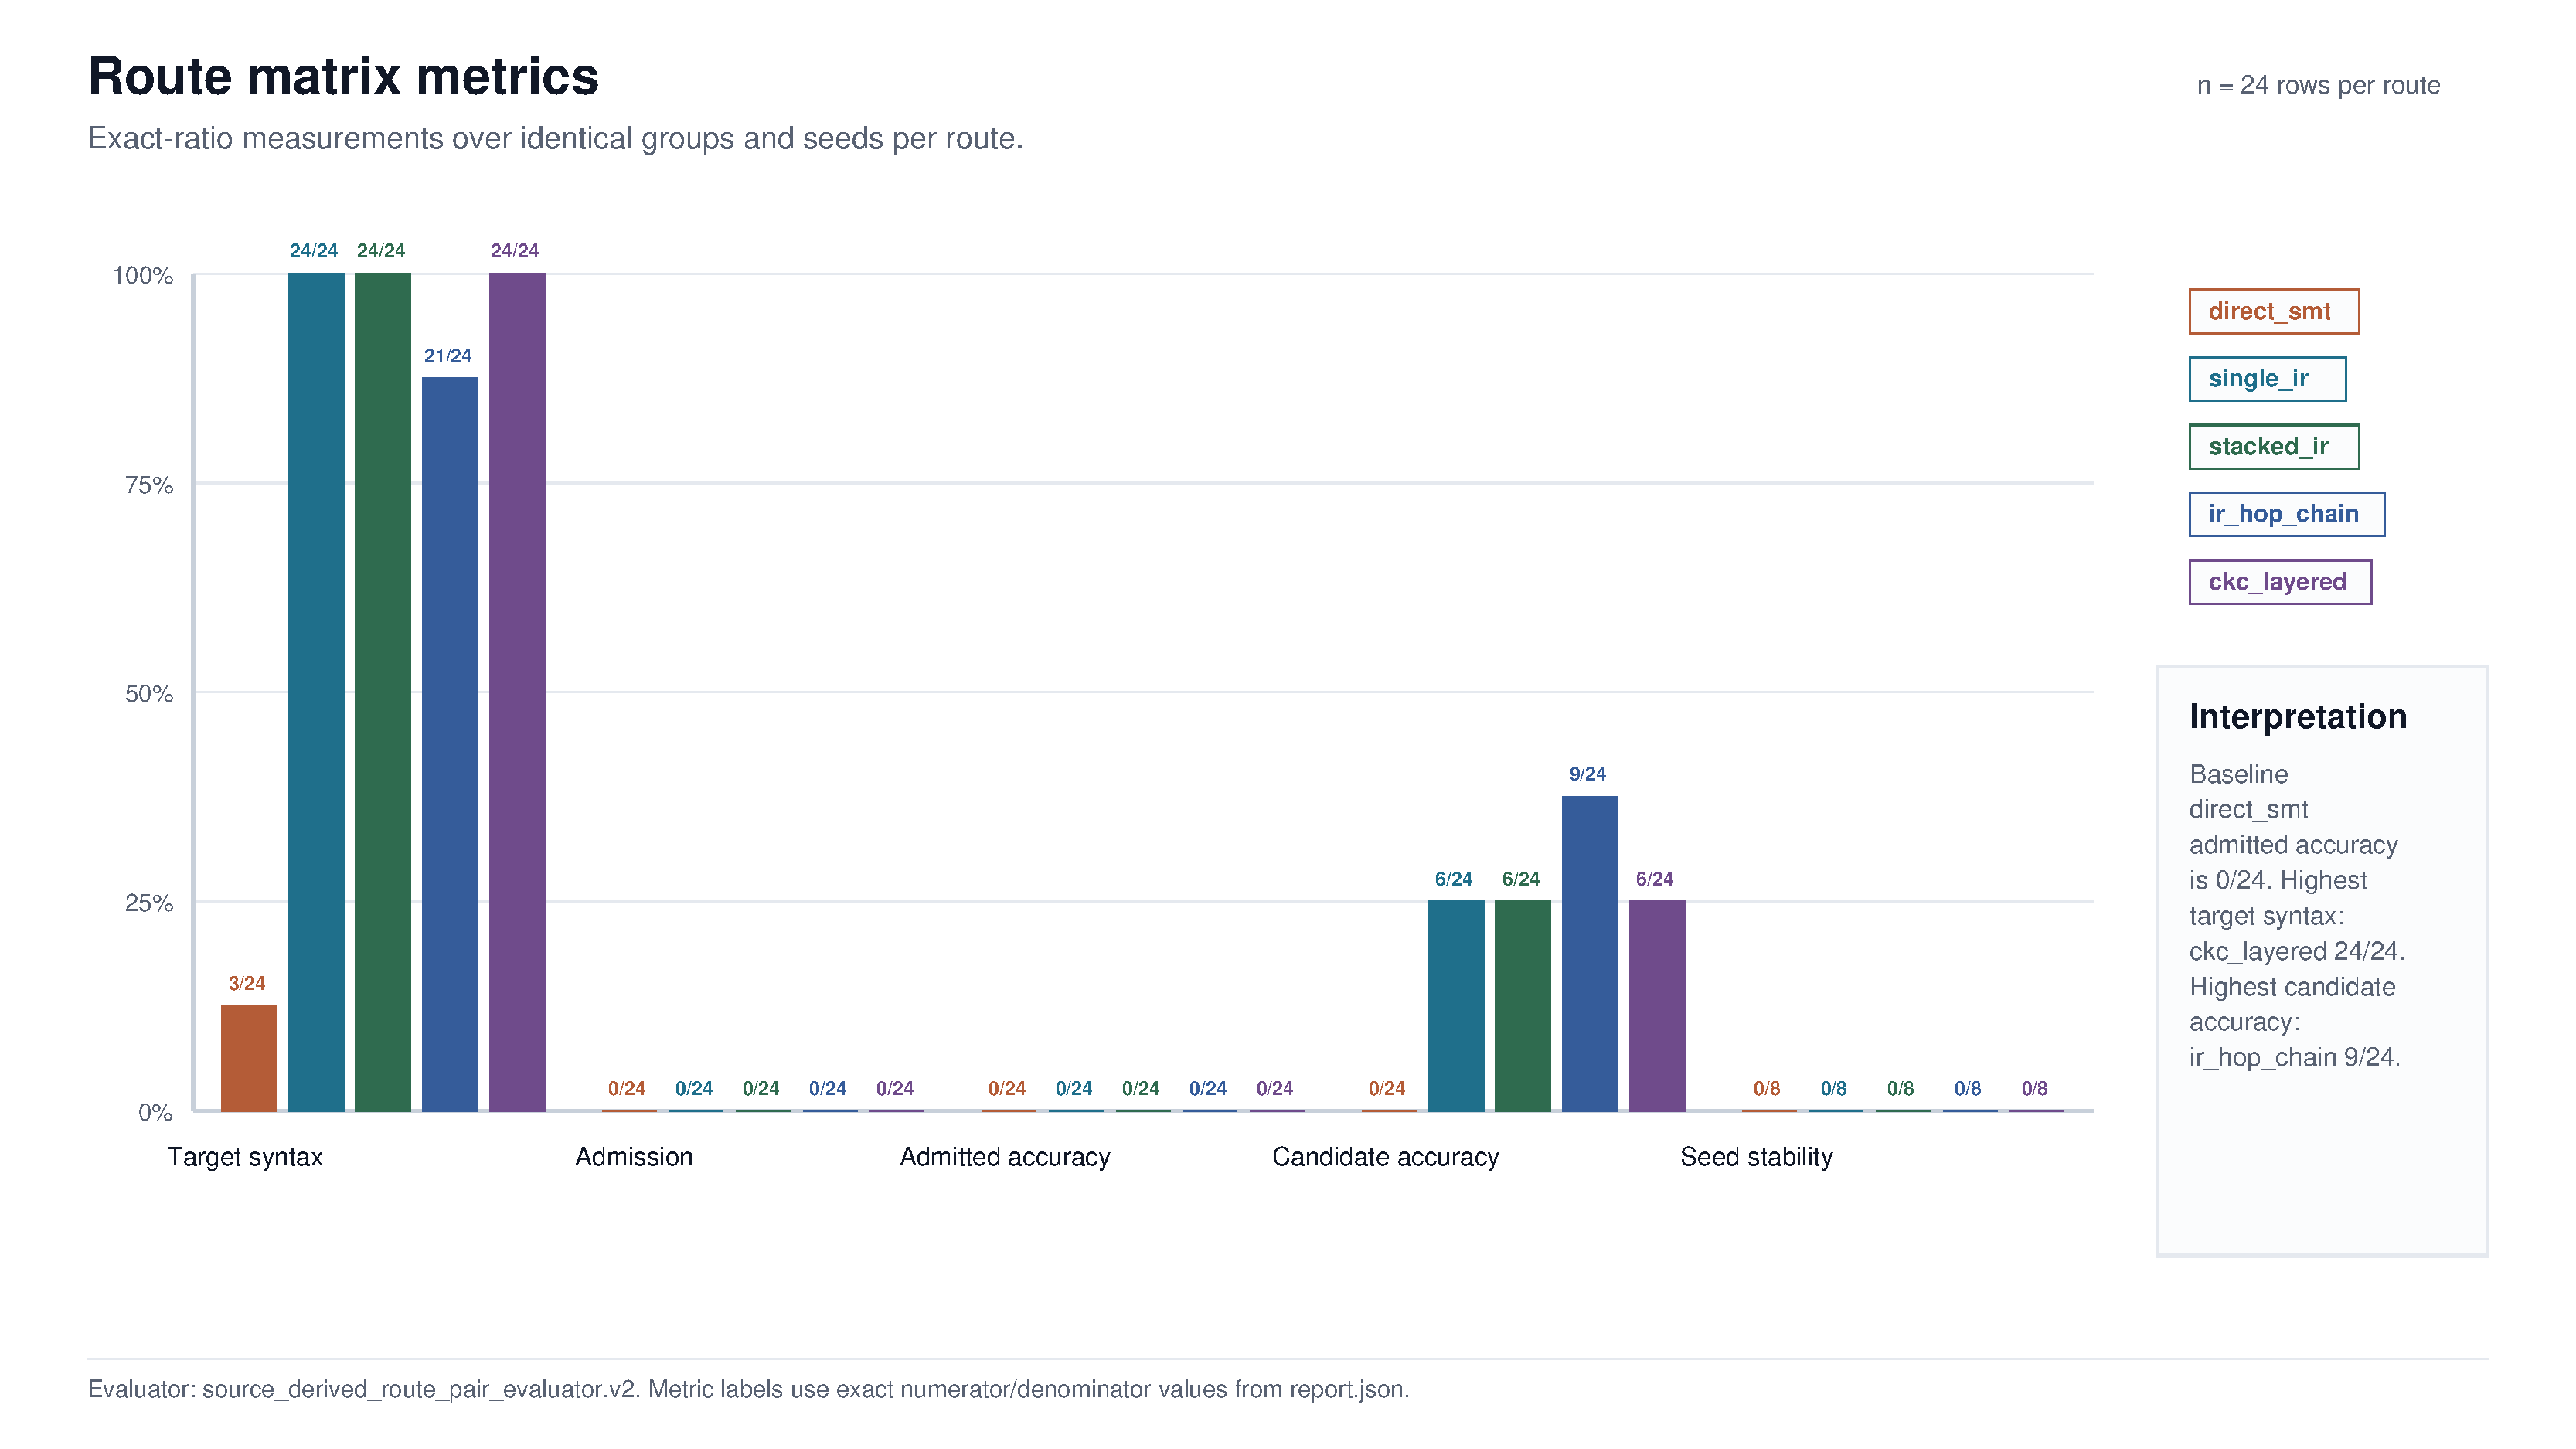
\includegraphics[width=\linewidth]{figures/manuscript/fig02_route_metrics.pdf}
  \caption{Route metrics from the current run, shown as exact-ratio profile lines over the route matrix with direct SMT retained as baseline. Candidate verdict accuracy is rejected-output audit evidence, not admitted baseline improvement.}
  \label{fig:route-metrics}
\end{figure}

\begin{figure}[t]
  \centering
  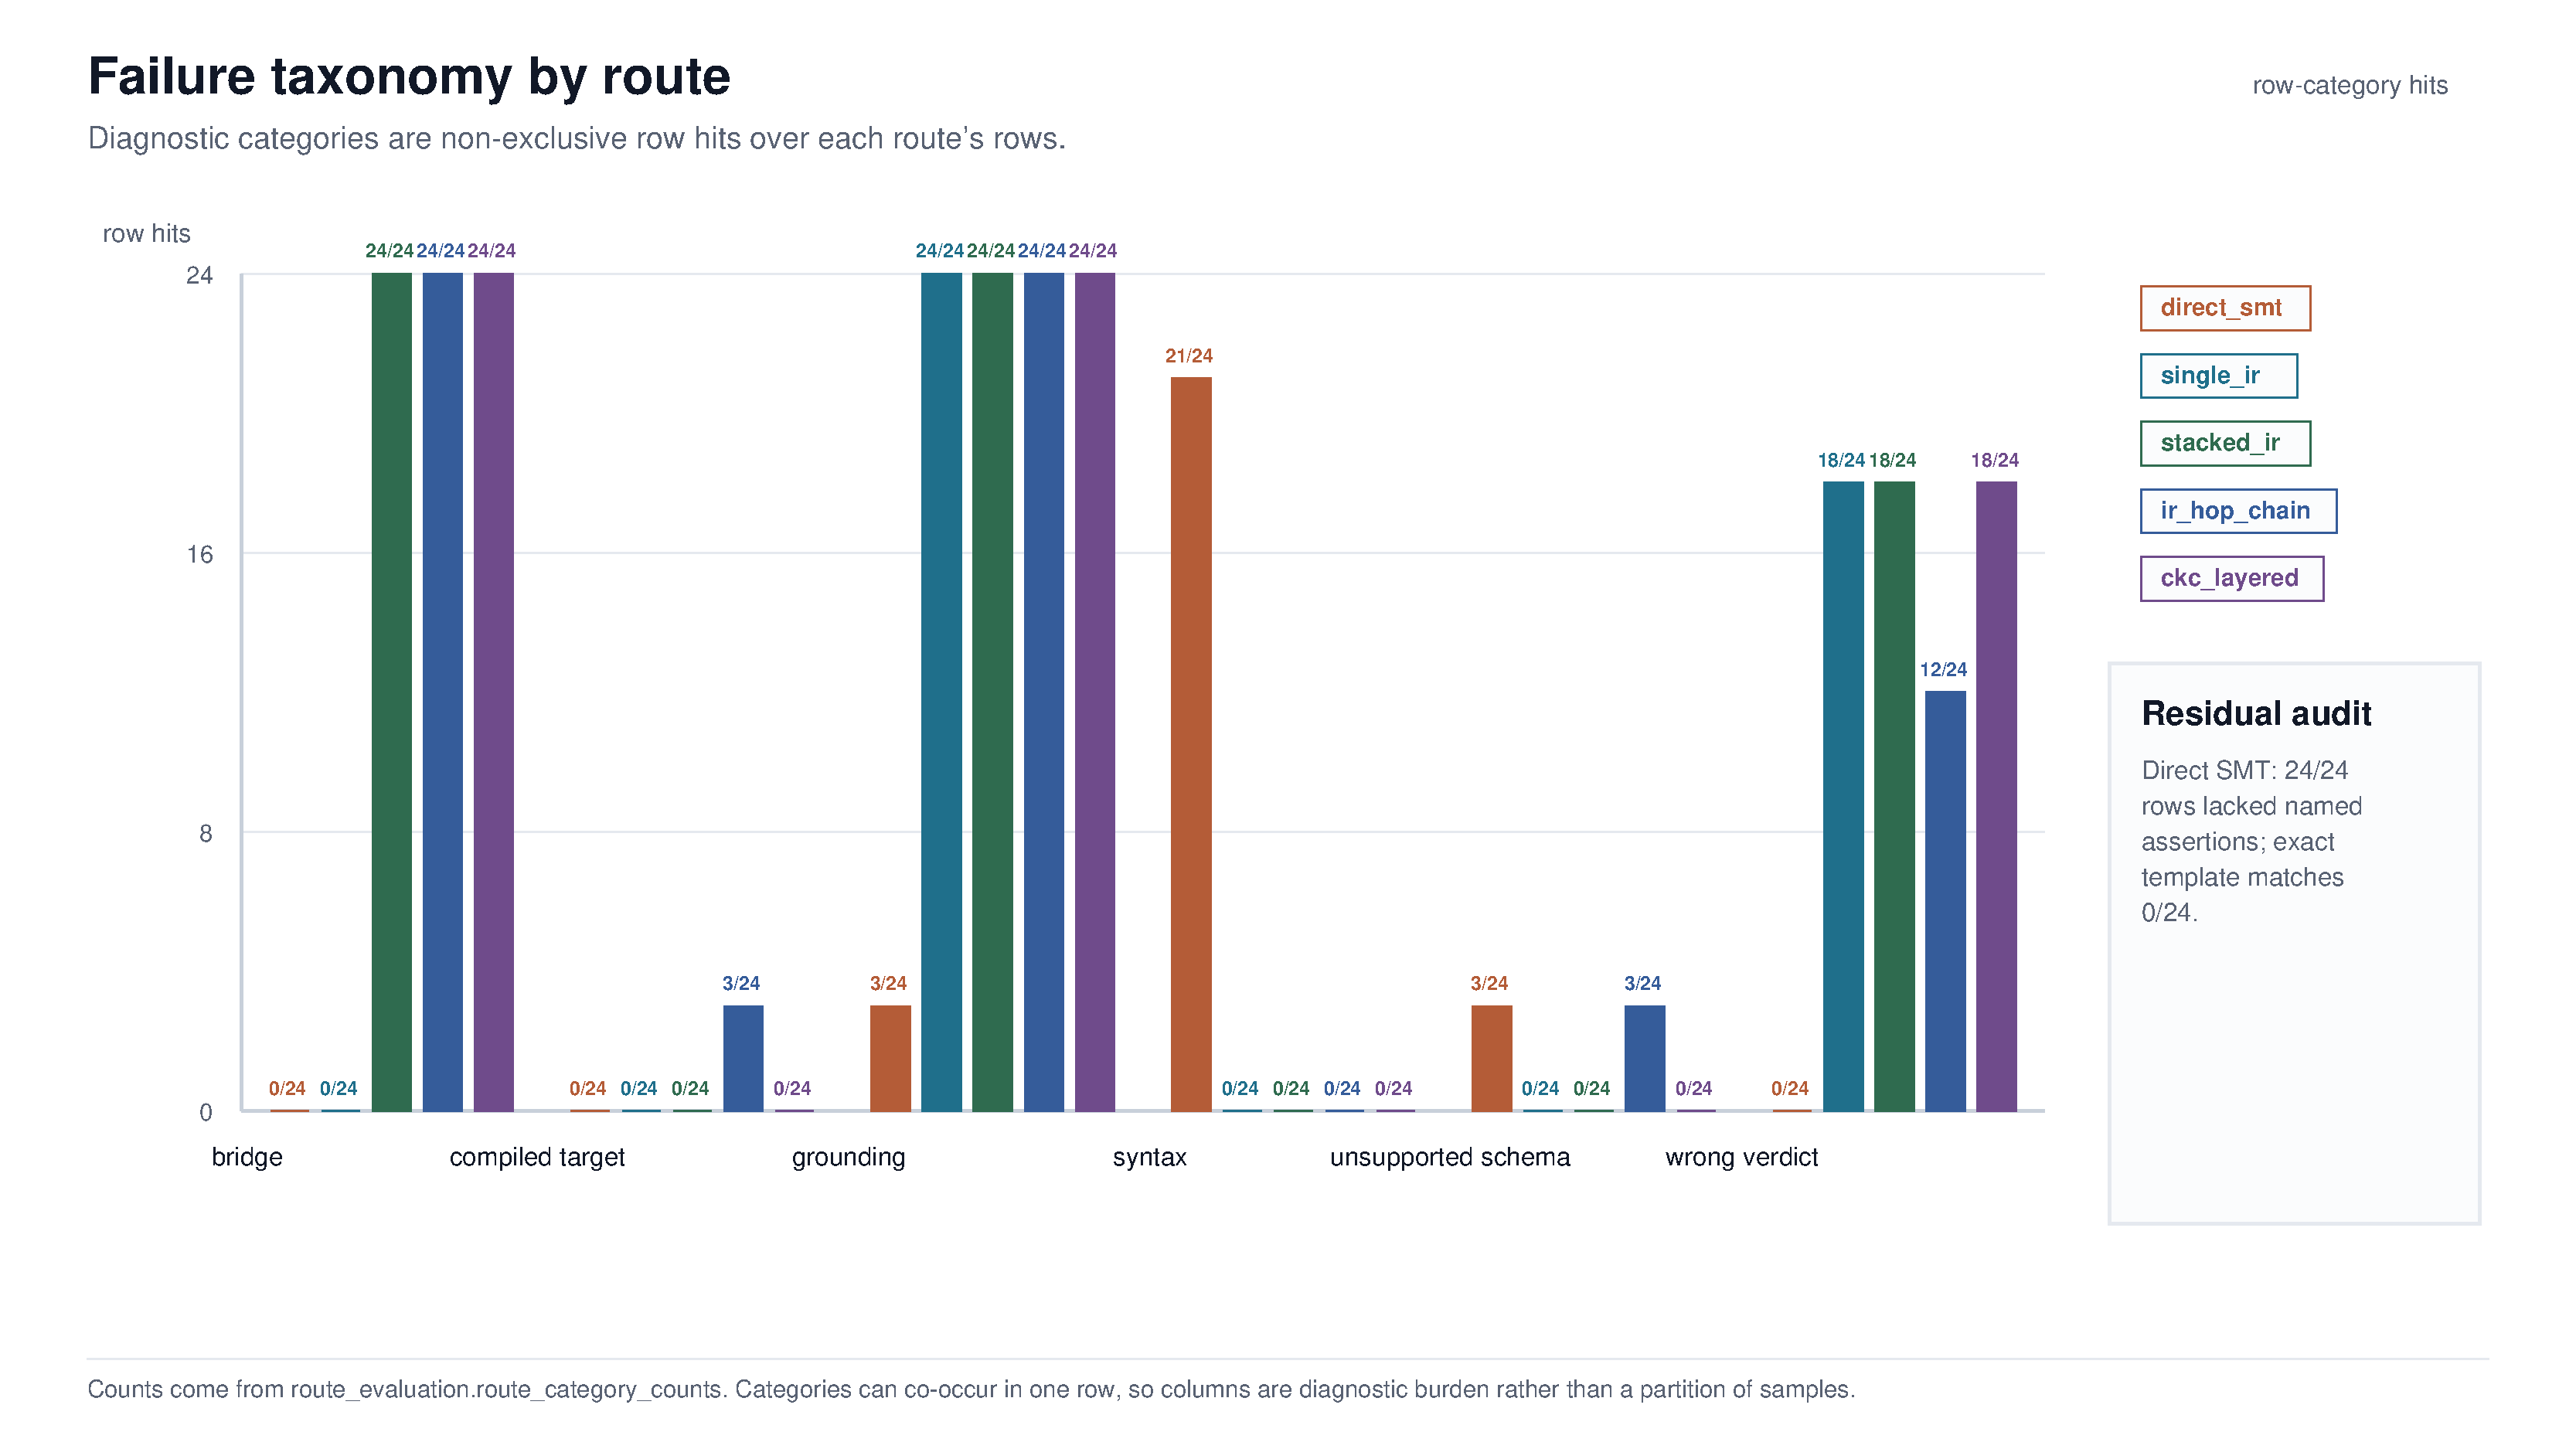
\includegraphics[width=\linewidth]{figures/manuscript/fig03_failure_taxonomy.pdf}
  \caption{Diagnostic row-category hits are shown as route profiles over the route matrix. Categories can co-occur, so profiles show diagnostic burden rather than a partition of samples.}
  \label{fig:failure-taxonomy}
\end{figure}

\begin{figure}[t]
  \centering
  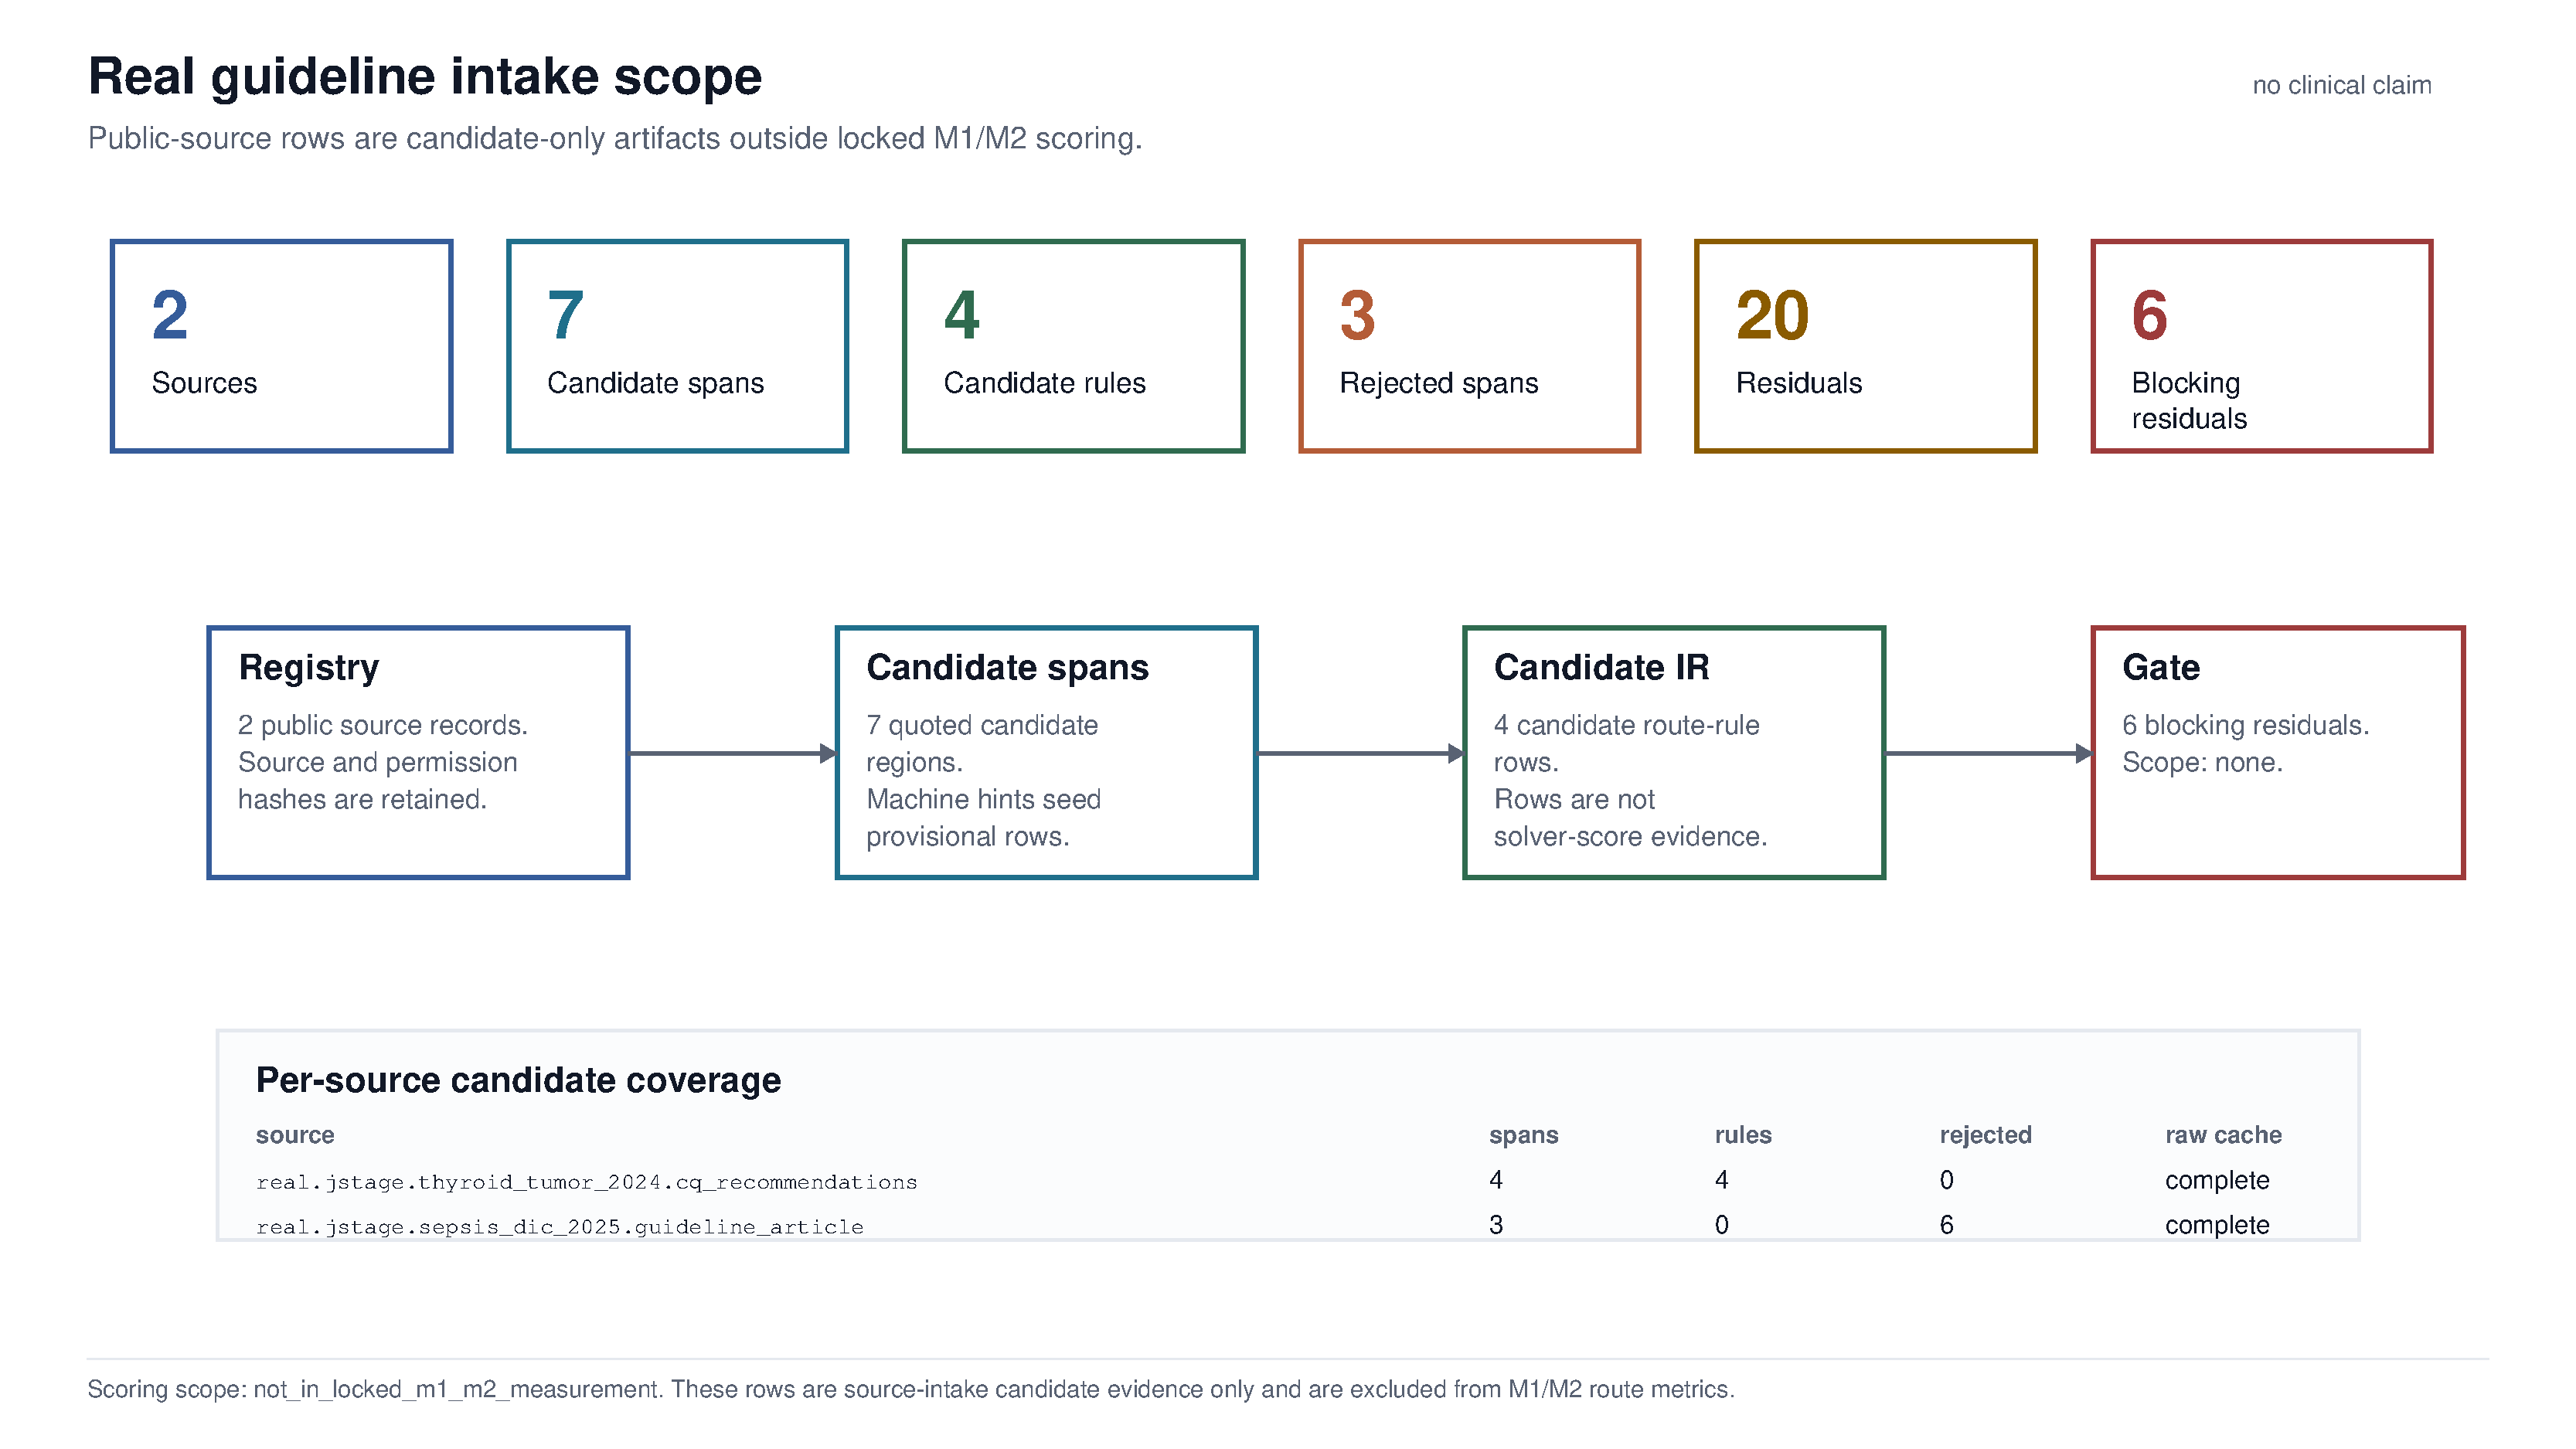
\includegraphics[width=\linewidth]{figures/manuscript/fig04_real_source_intake.pdf}
  \caption{Real Japanese guideline sources are represented as candidate-only source-intake artifacts with source and permission hashes, but they remain outside locked M1/M2 scoring and carry no clinical claim.}
  \label{fig:real-source-intake}
\end{figure}

\begin{figure}[t]
  \centering
  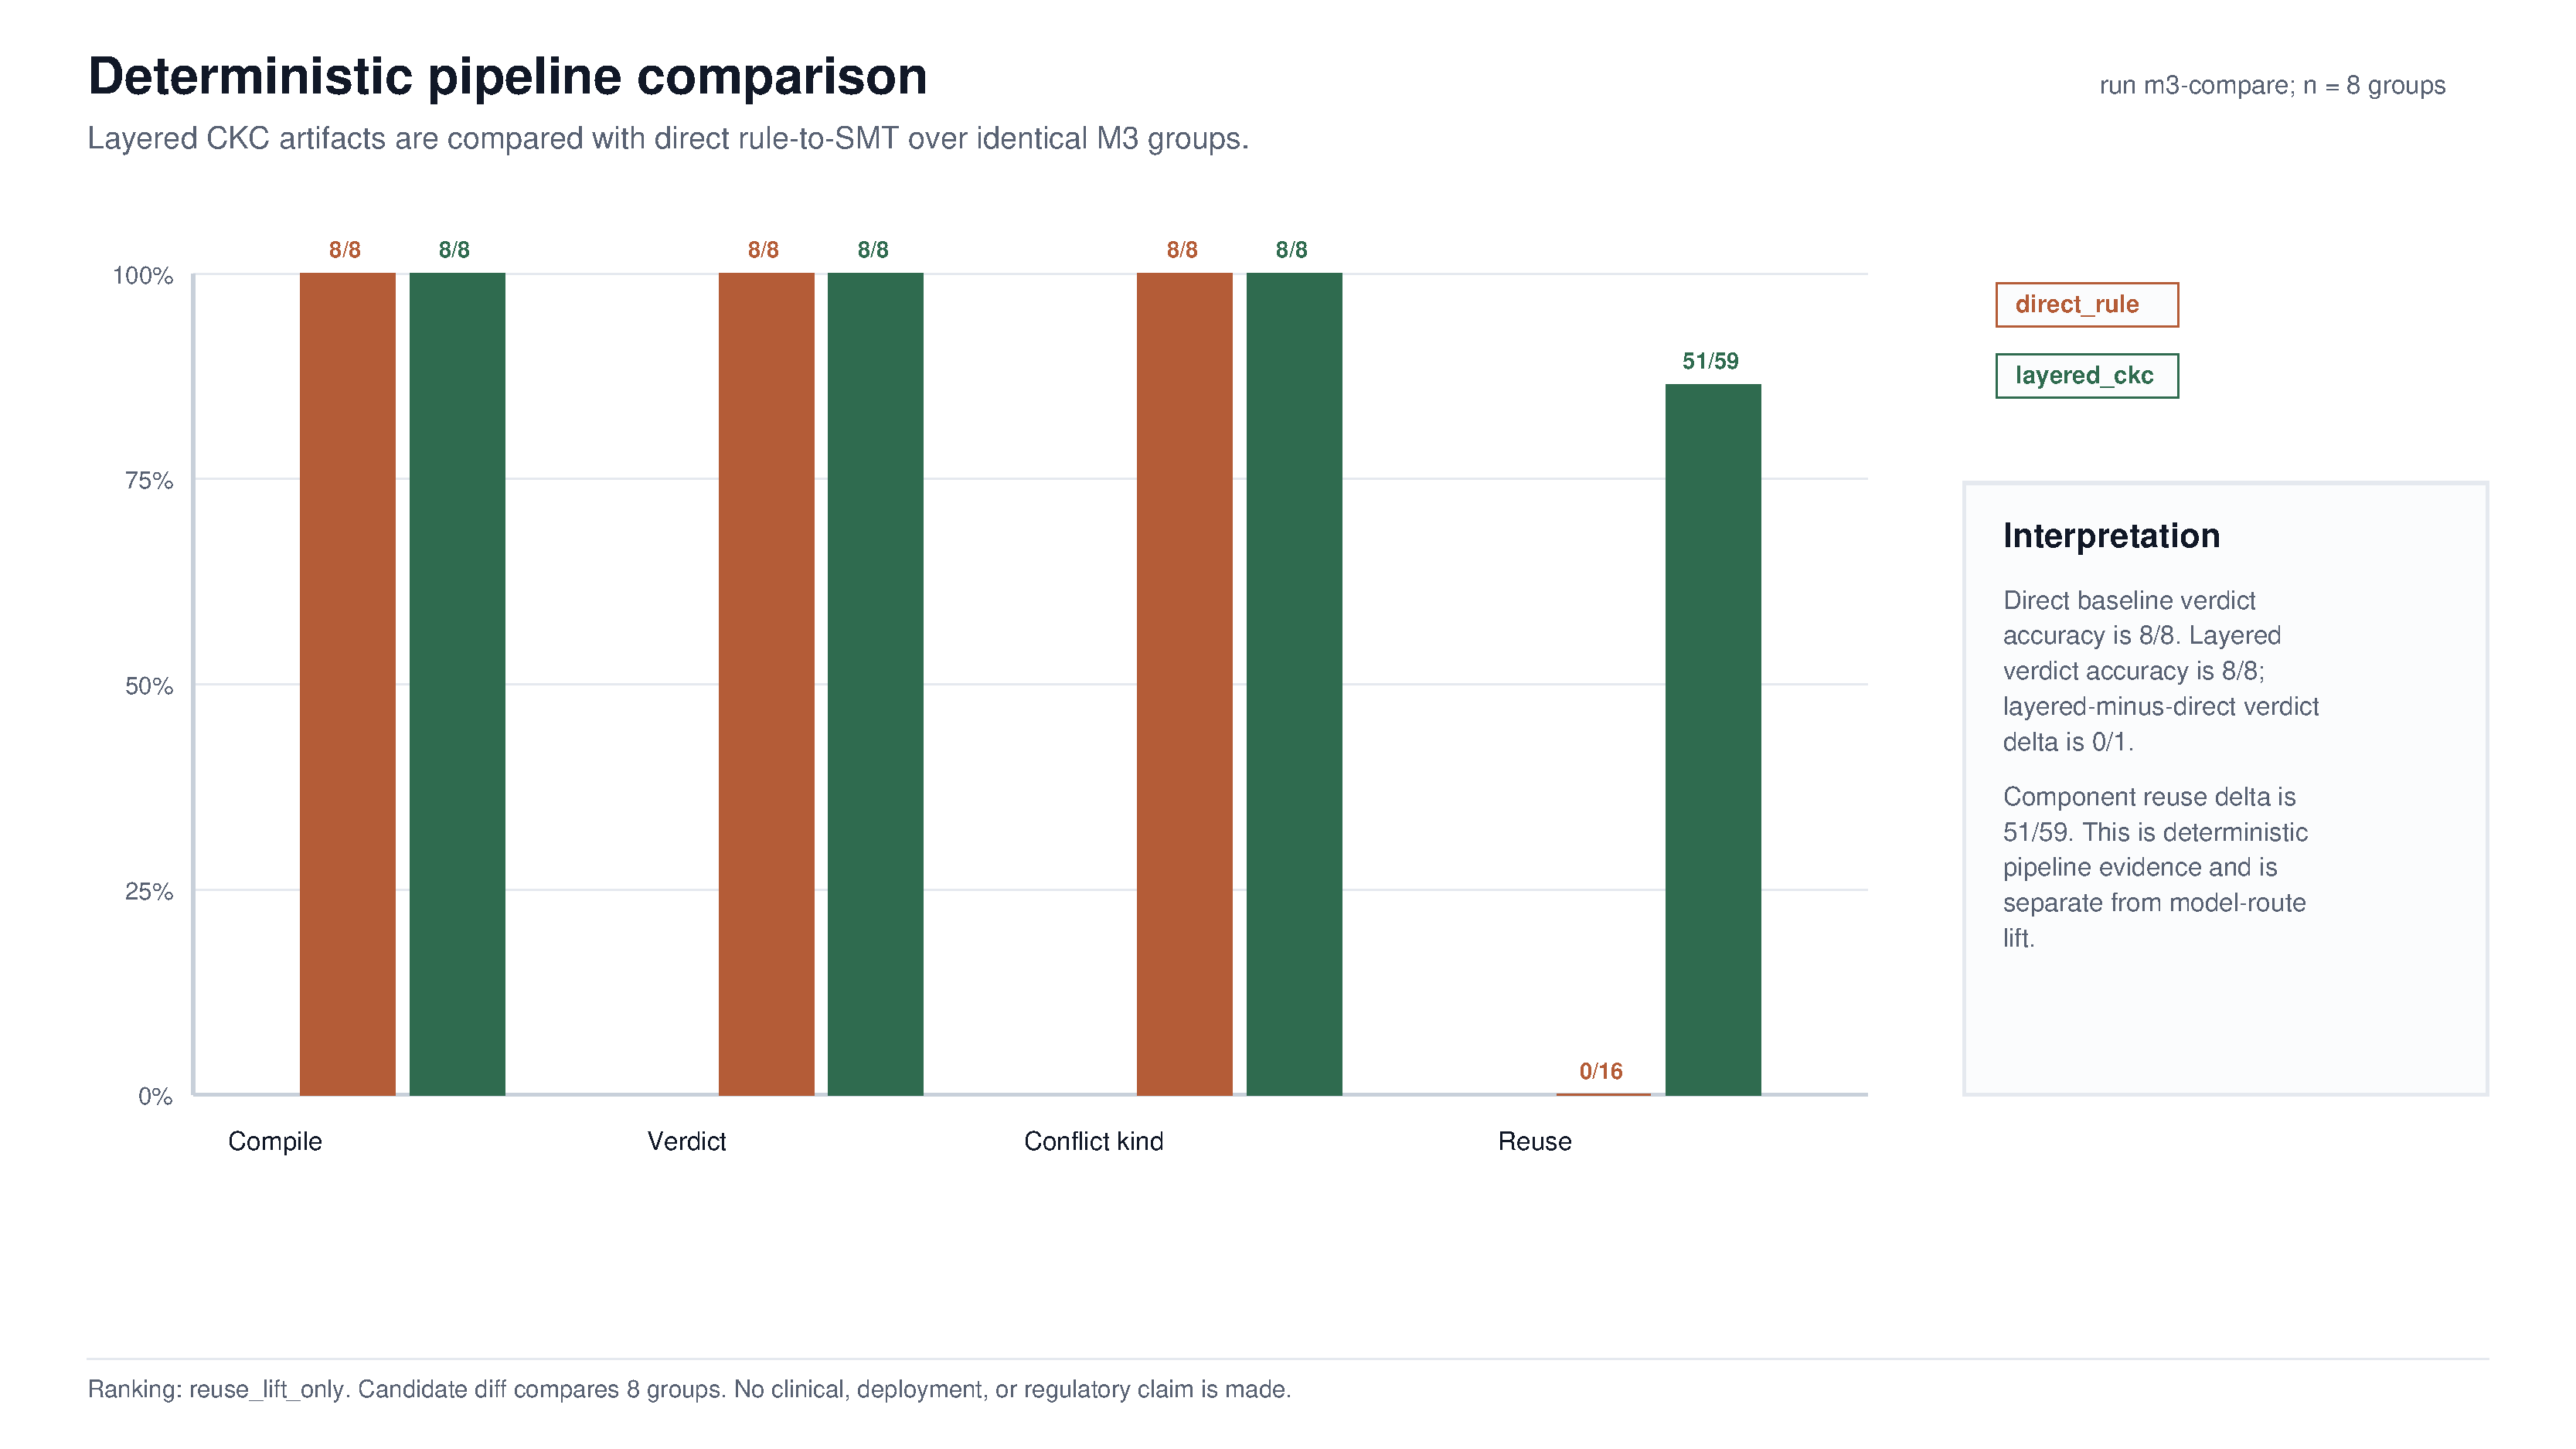
\includegraphics[width=\linewidth]{figures/manuscript/fig05_pipeline_comparison.pdf}
  \caption{Deterministic pipeline comparison. Direct rule-to-SMT is retained as baseline; profile lines show that the layered CKC pipeline matches verdict and conflict-kind accuracy in the current M3 comparison while component reuse is reported separately from model-route baseline deltas.}
  \label{fig:pipeline-comparison}
\end{figure}

\begin{figure}[t]
  \centering
  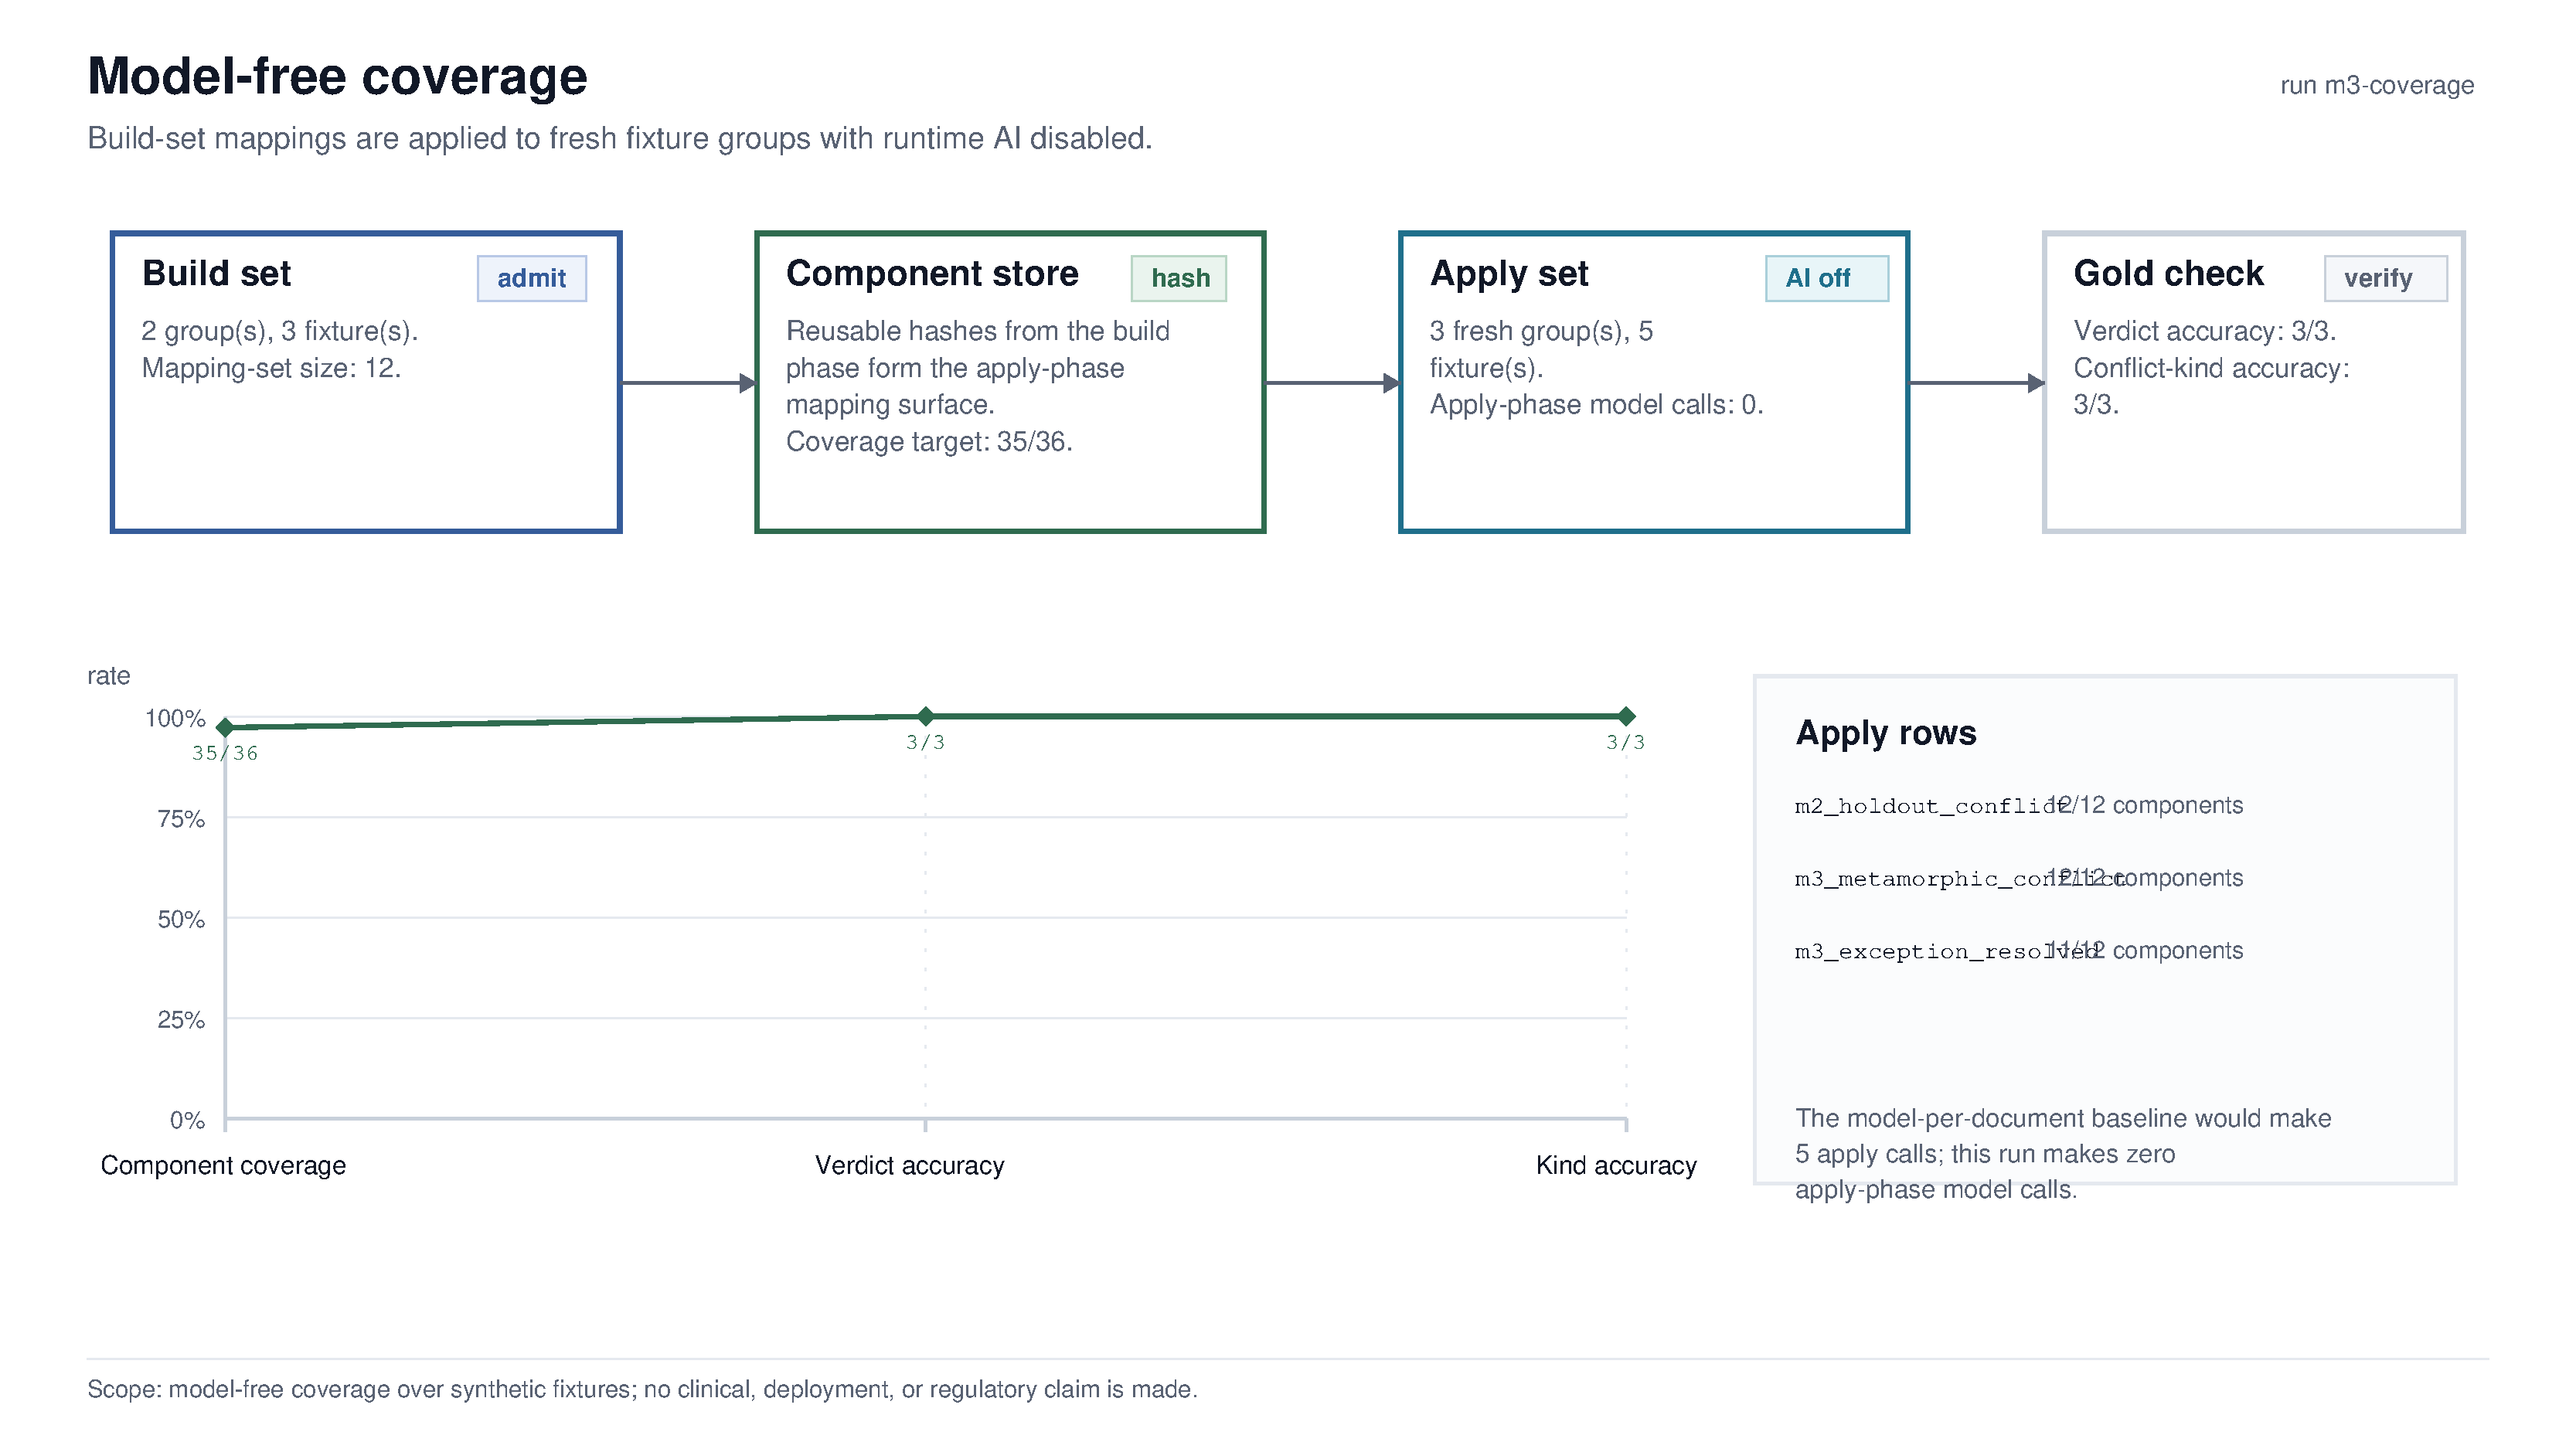
\includegraphics[width=\linewidth]{figures/manuscript/fig06_model_free_coverage.pdf}
  \caption{Model-free coverage. Build-set mappings are applied to fresh synthetic fixture groups with runtime AI disabled; component coverage, verdict accuracy, and zero apply-phase model calls are reported as exact ratios/counts.}
  \label{fig:model-free-coverage}
\end{figure}
 or copy individual figure blocks.

\begin{figure}[t]
  \centering
  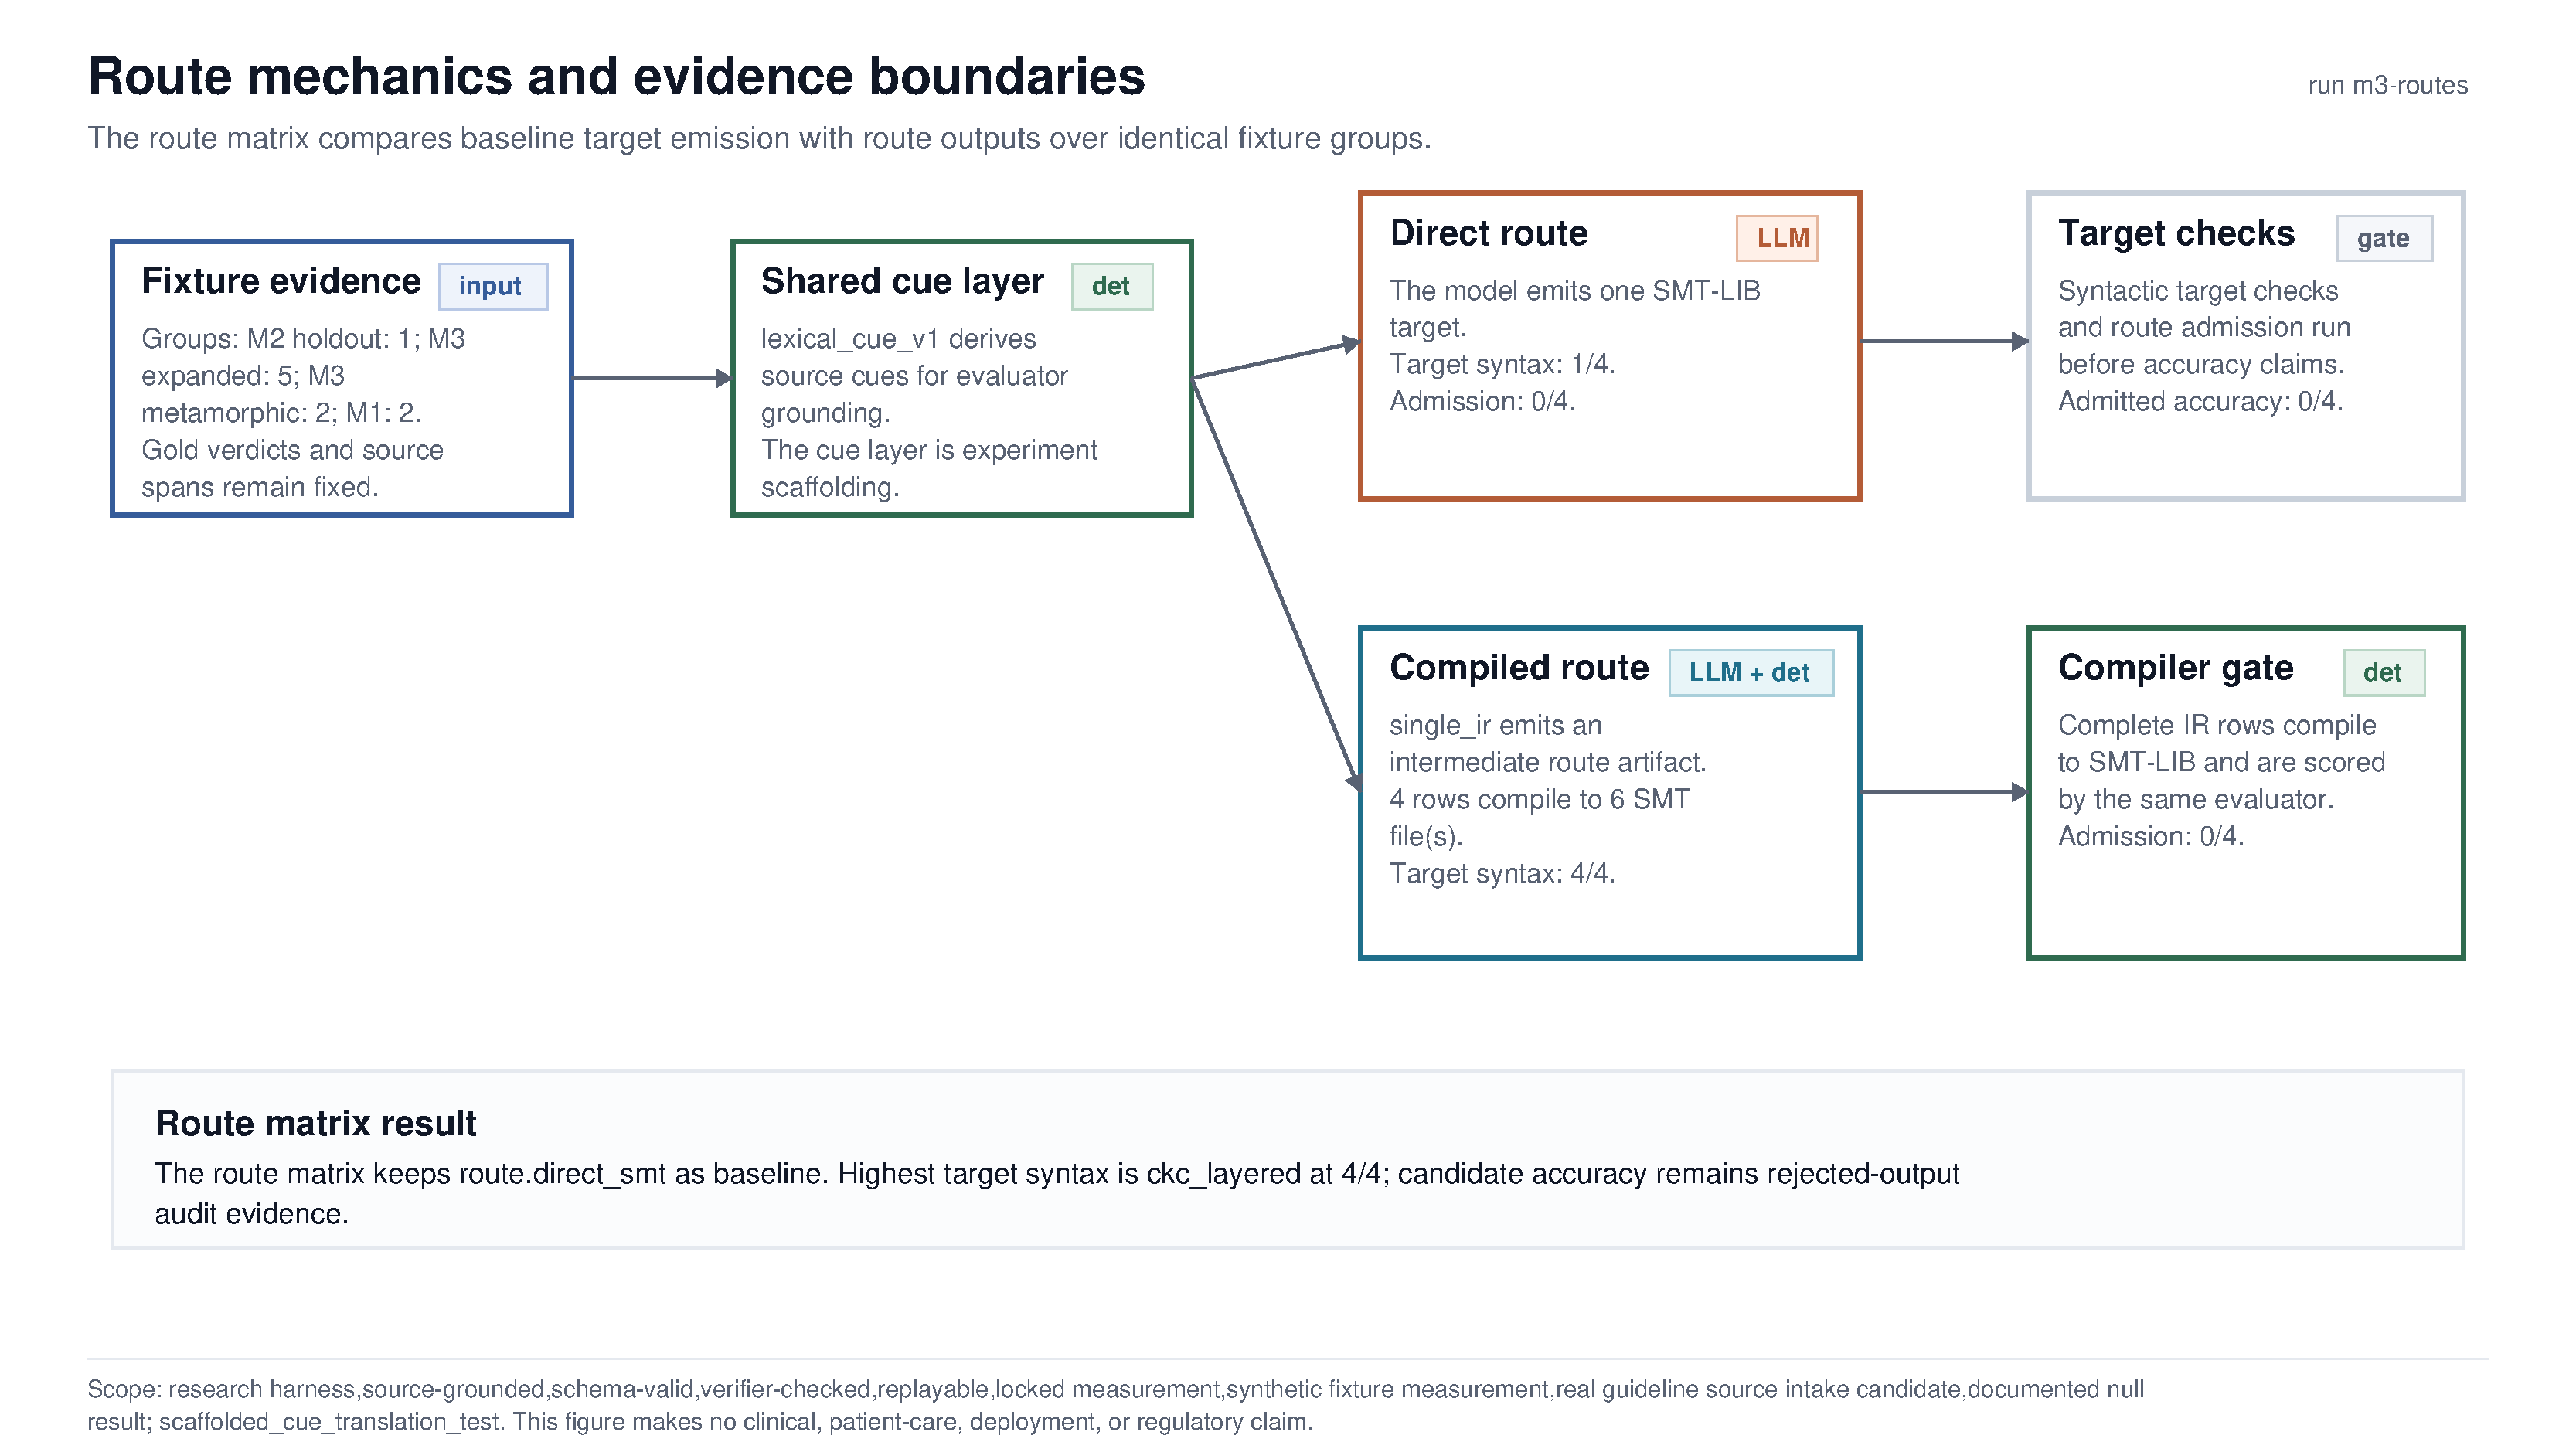
\includegraphics[width=\linewidth]{figures/manuscript/fig01_route_mechanics.pdf}
  \caption{Route mechanics. Implemented routes consume the same fixture groups and are scored by the same evaluator; the current run shows a target-syntax baseline delta only, not an admitted-verdict baseline delta.}
  \label{fig:route-mechanics}
\end{figure}

\begin{figure}[t]
  \centering
  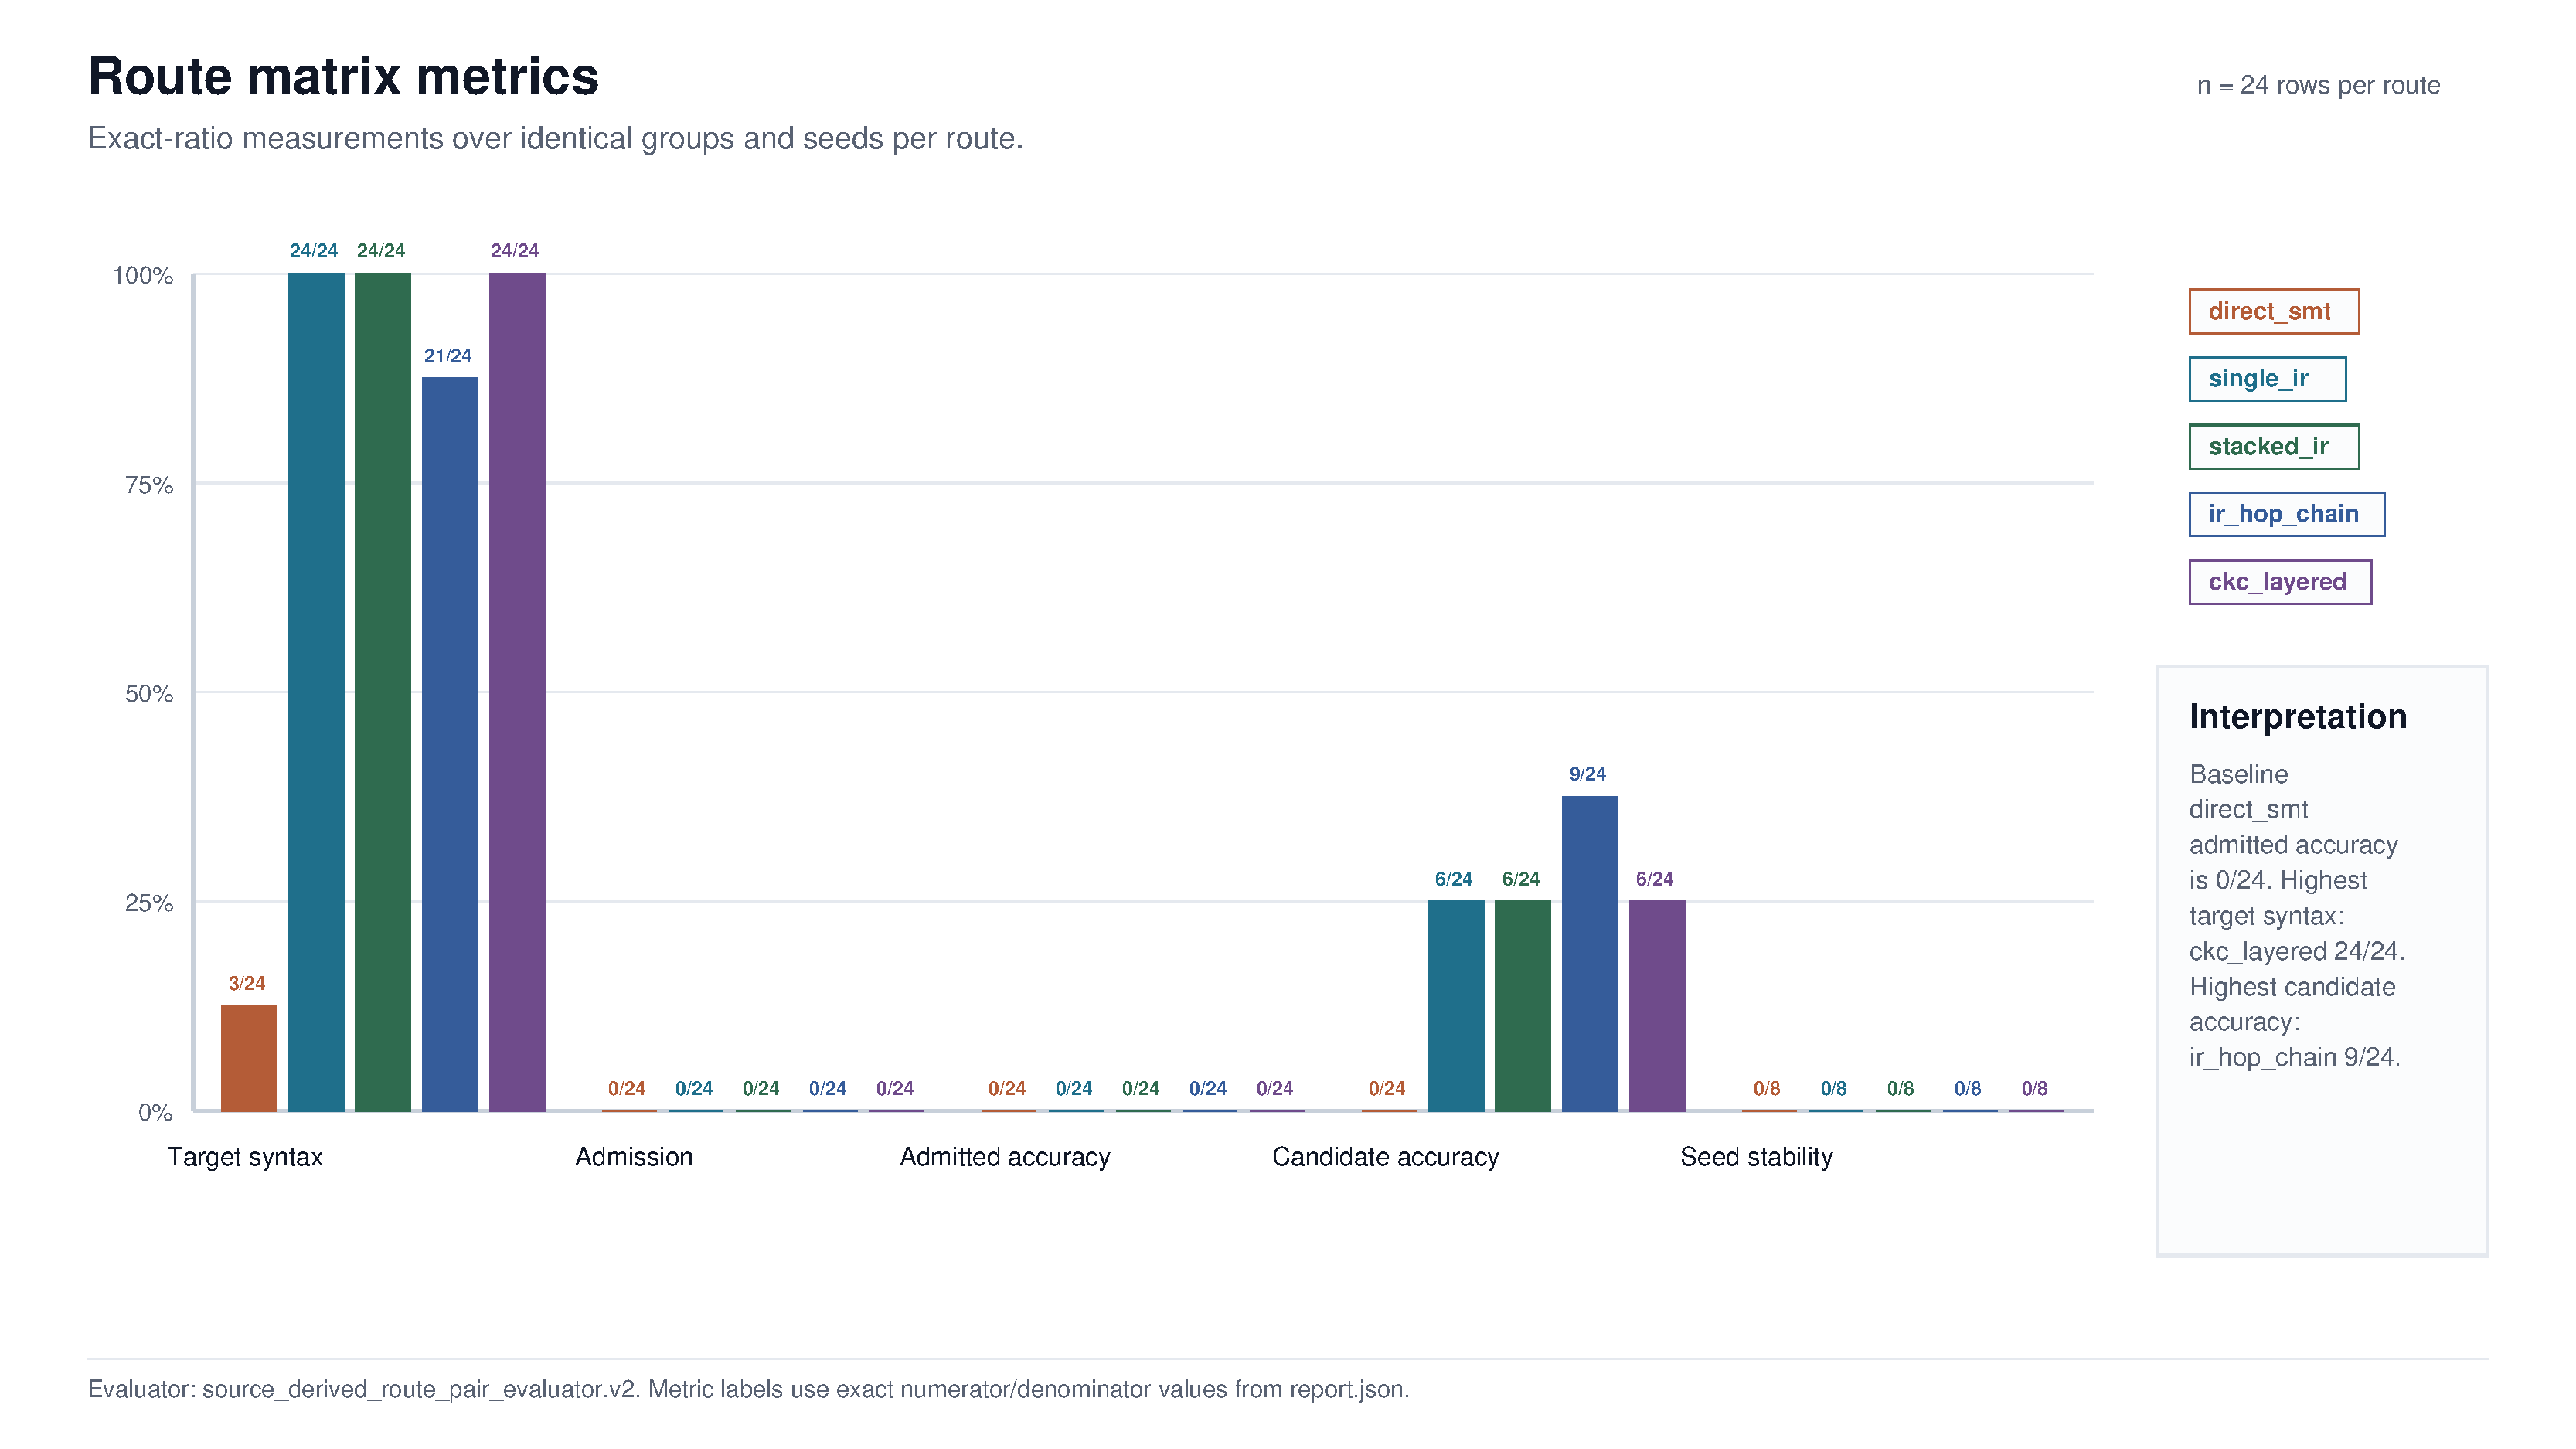
\includegraphics[width=\linewidth]{figures/manuscript/fig02_route_metrics.pdf}
  \caption{Route metrics from the current run, shown as exact-ratio profile lines over the route matrix with direct SMT retained as baseline. Candidate verdict accuracy is rejected-output audit evidence, not admitted baseline improvement.}
  \label{fig:route-metrics}
\end{figure}

\begin{figure}[t]
  \centering
  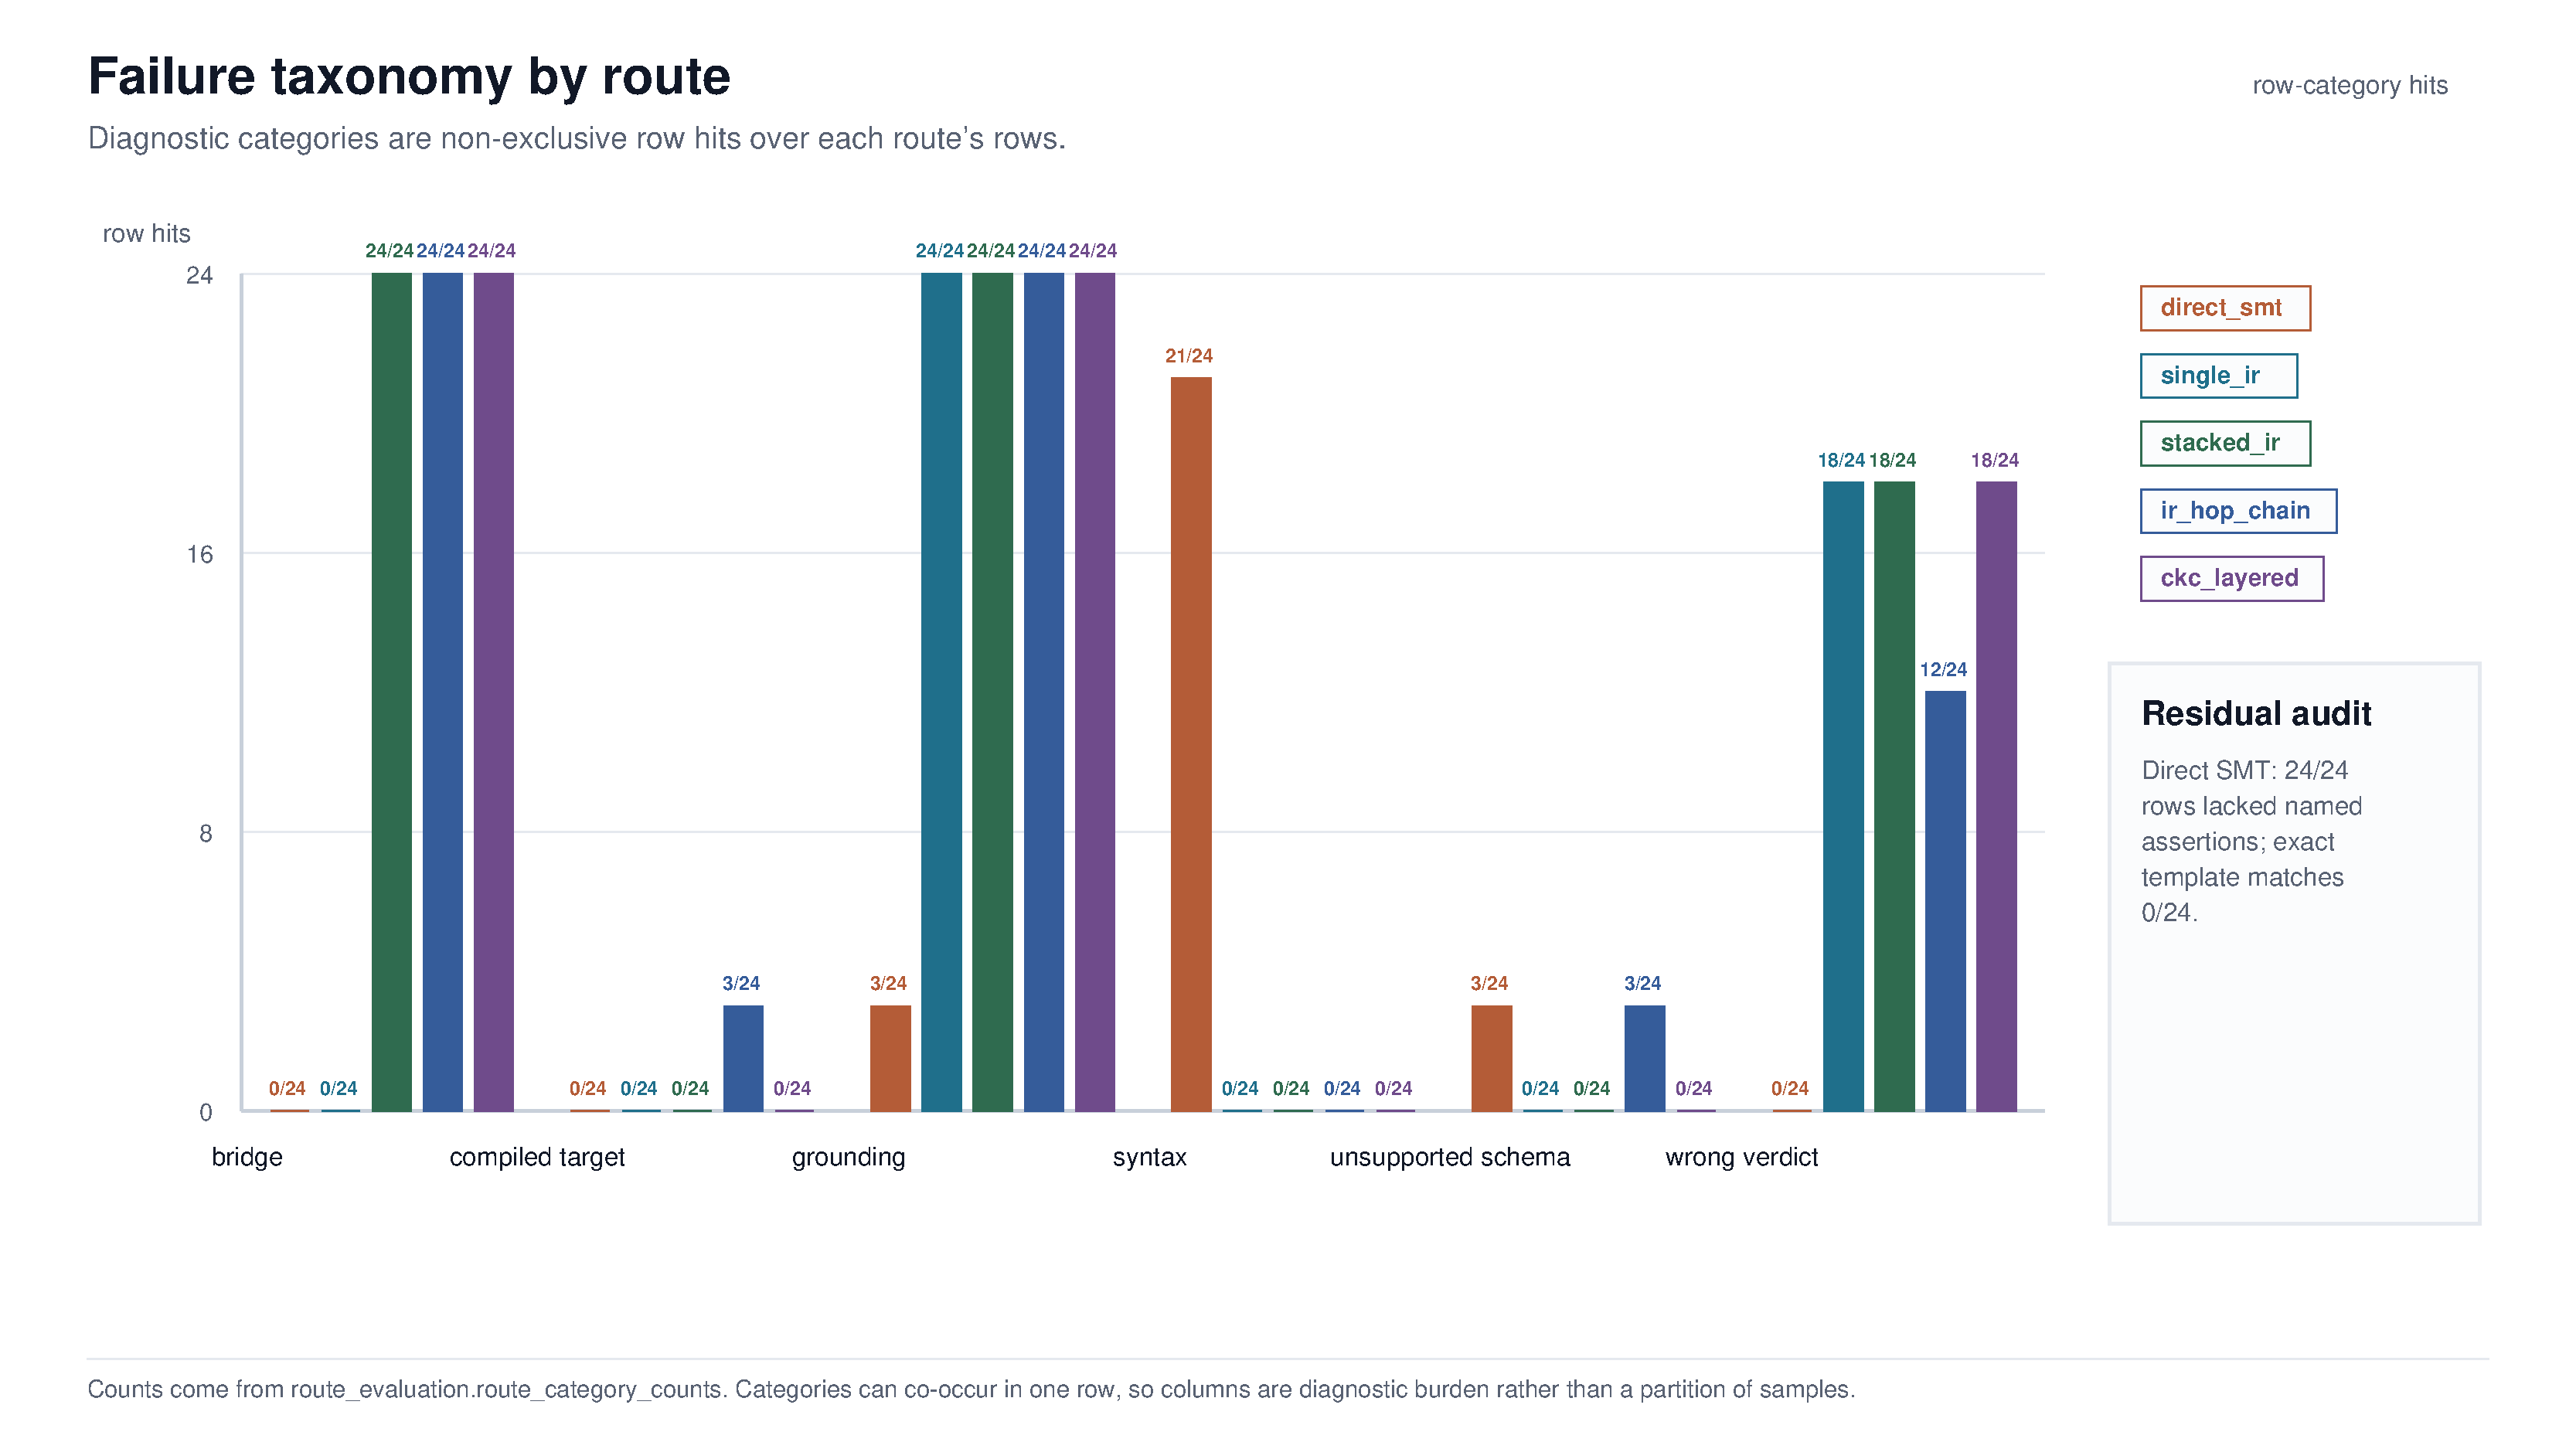
\includegraphics[width=\linewidth]{figures/manuscript/fig03_failure_taxonomy.pdf}
  \caption{Diagnostic row-category hits are shown as route profiles over the route matrix. Categories can co-occur, so profiles show diagnostic burden rather than a partition of samples.}
  \label{fig:failure-taxonomy}
\end{figure}

\begin{figure}[t]
  \centering
  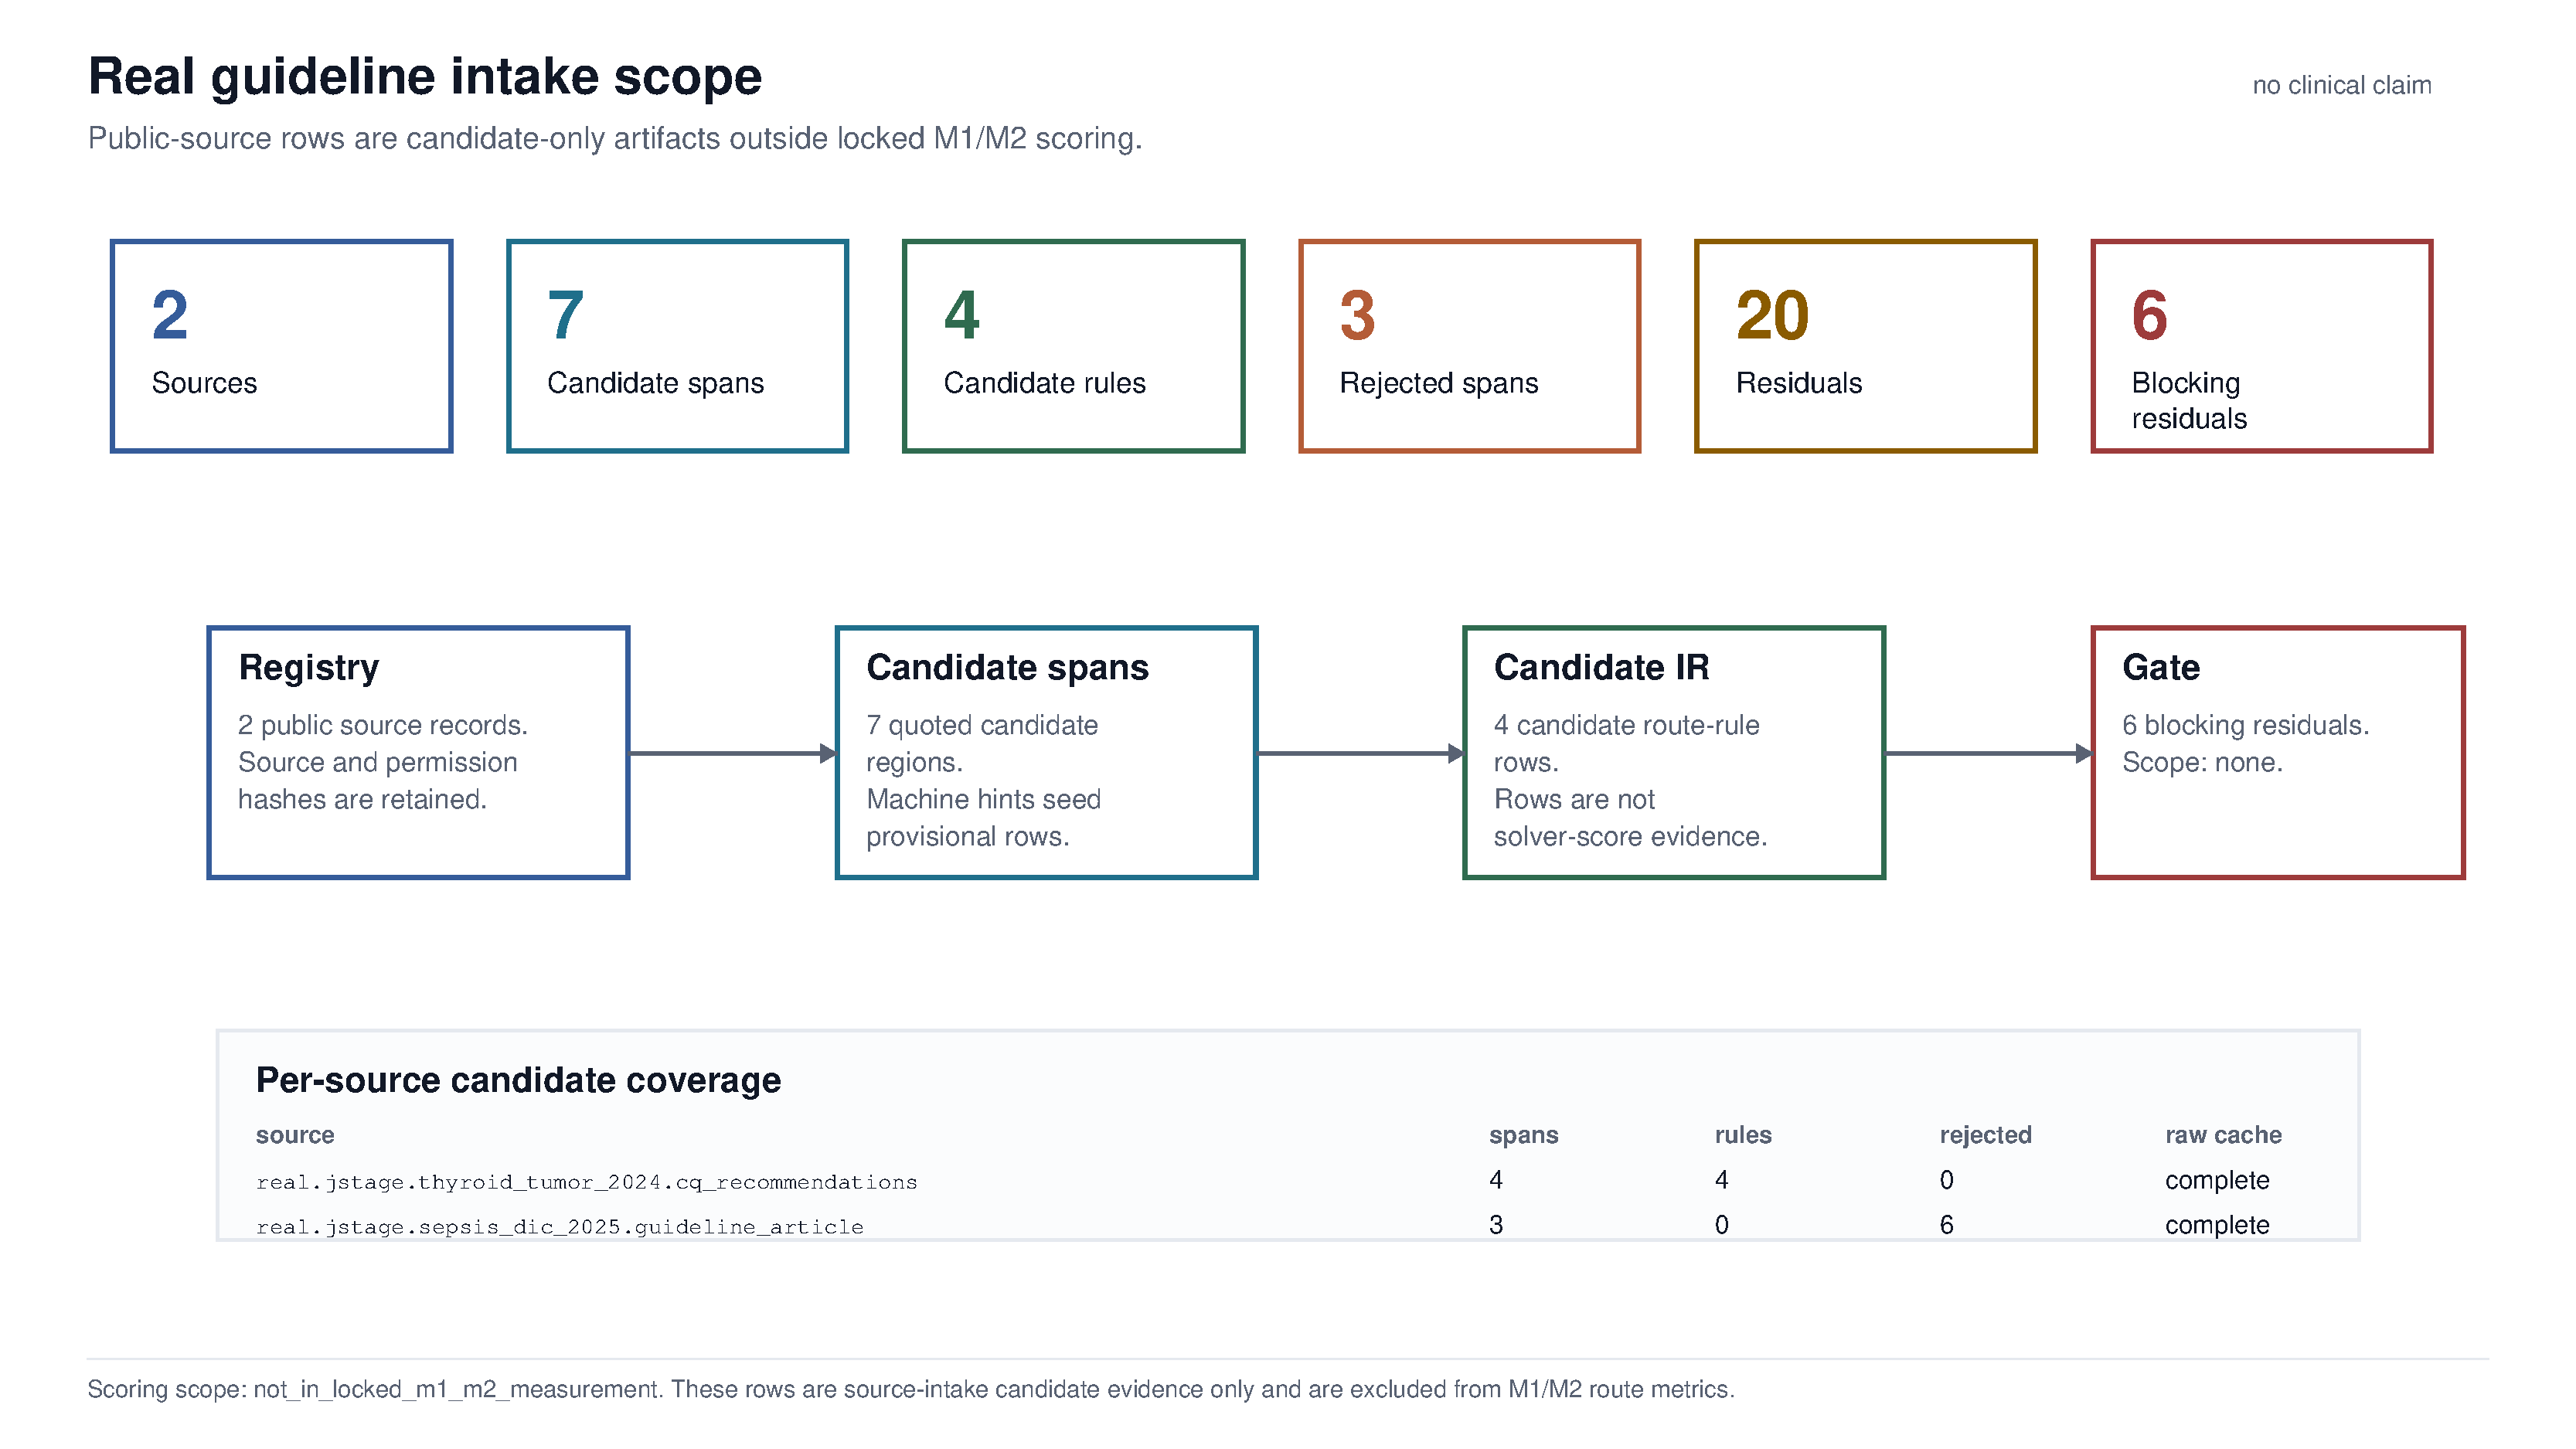
\includegraphics[width=\linewidth]{figures/manuscript/fig04_real_source_intake.pdf}
  \caption{Real Japanese guideline sources are represented as candidate-only source-intake artifacts with source and permission hashes, but they remain outside locked M1/M2 scoring and carry no clinical claim.}
  \label{fig:real-source-intake}
\end{figure}

\begin{figure}[t]
  \centering
  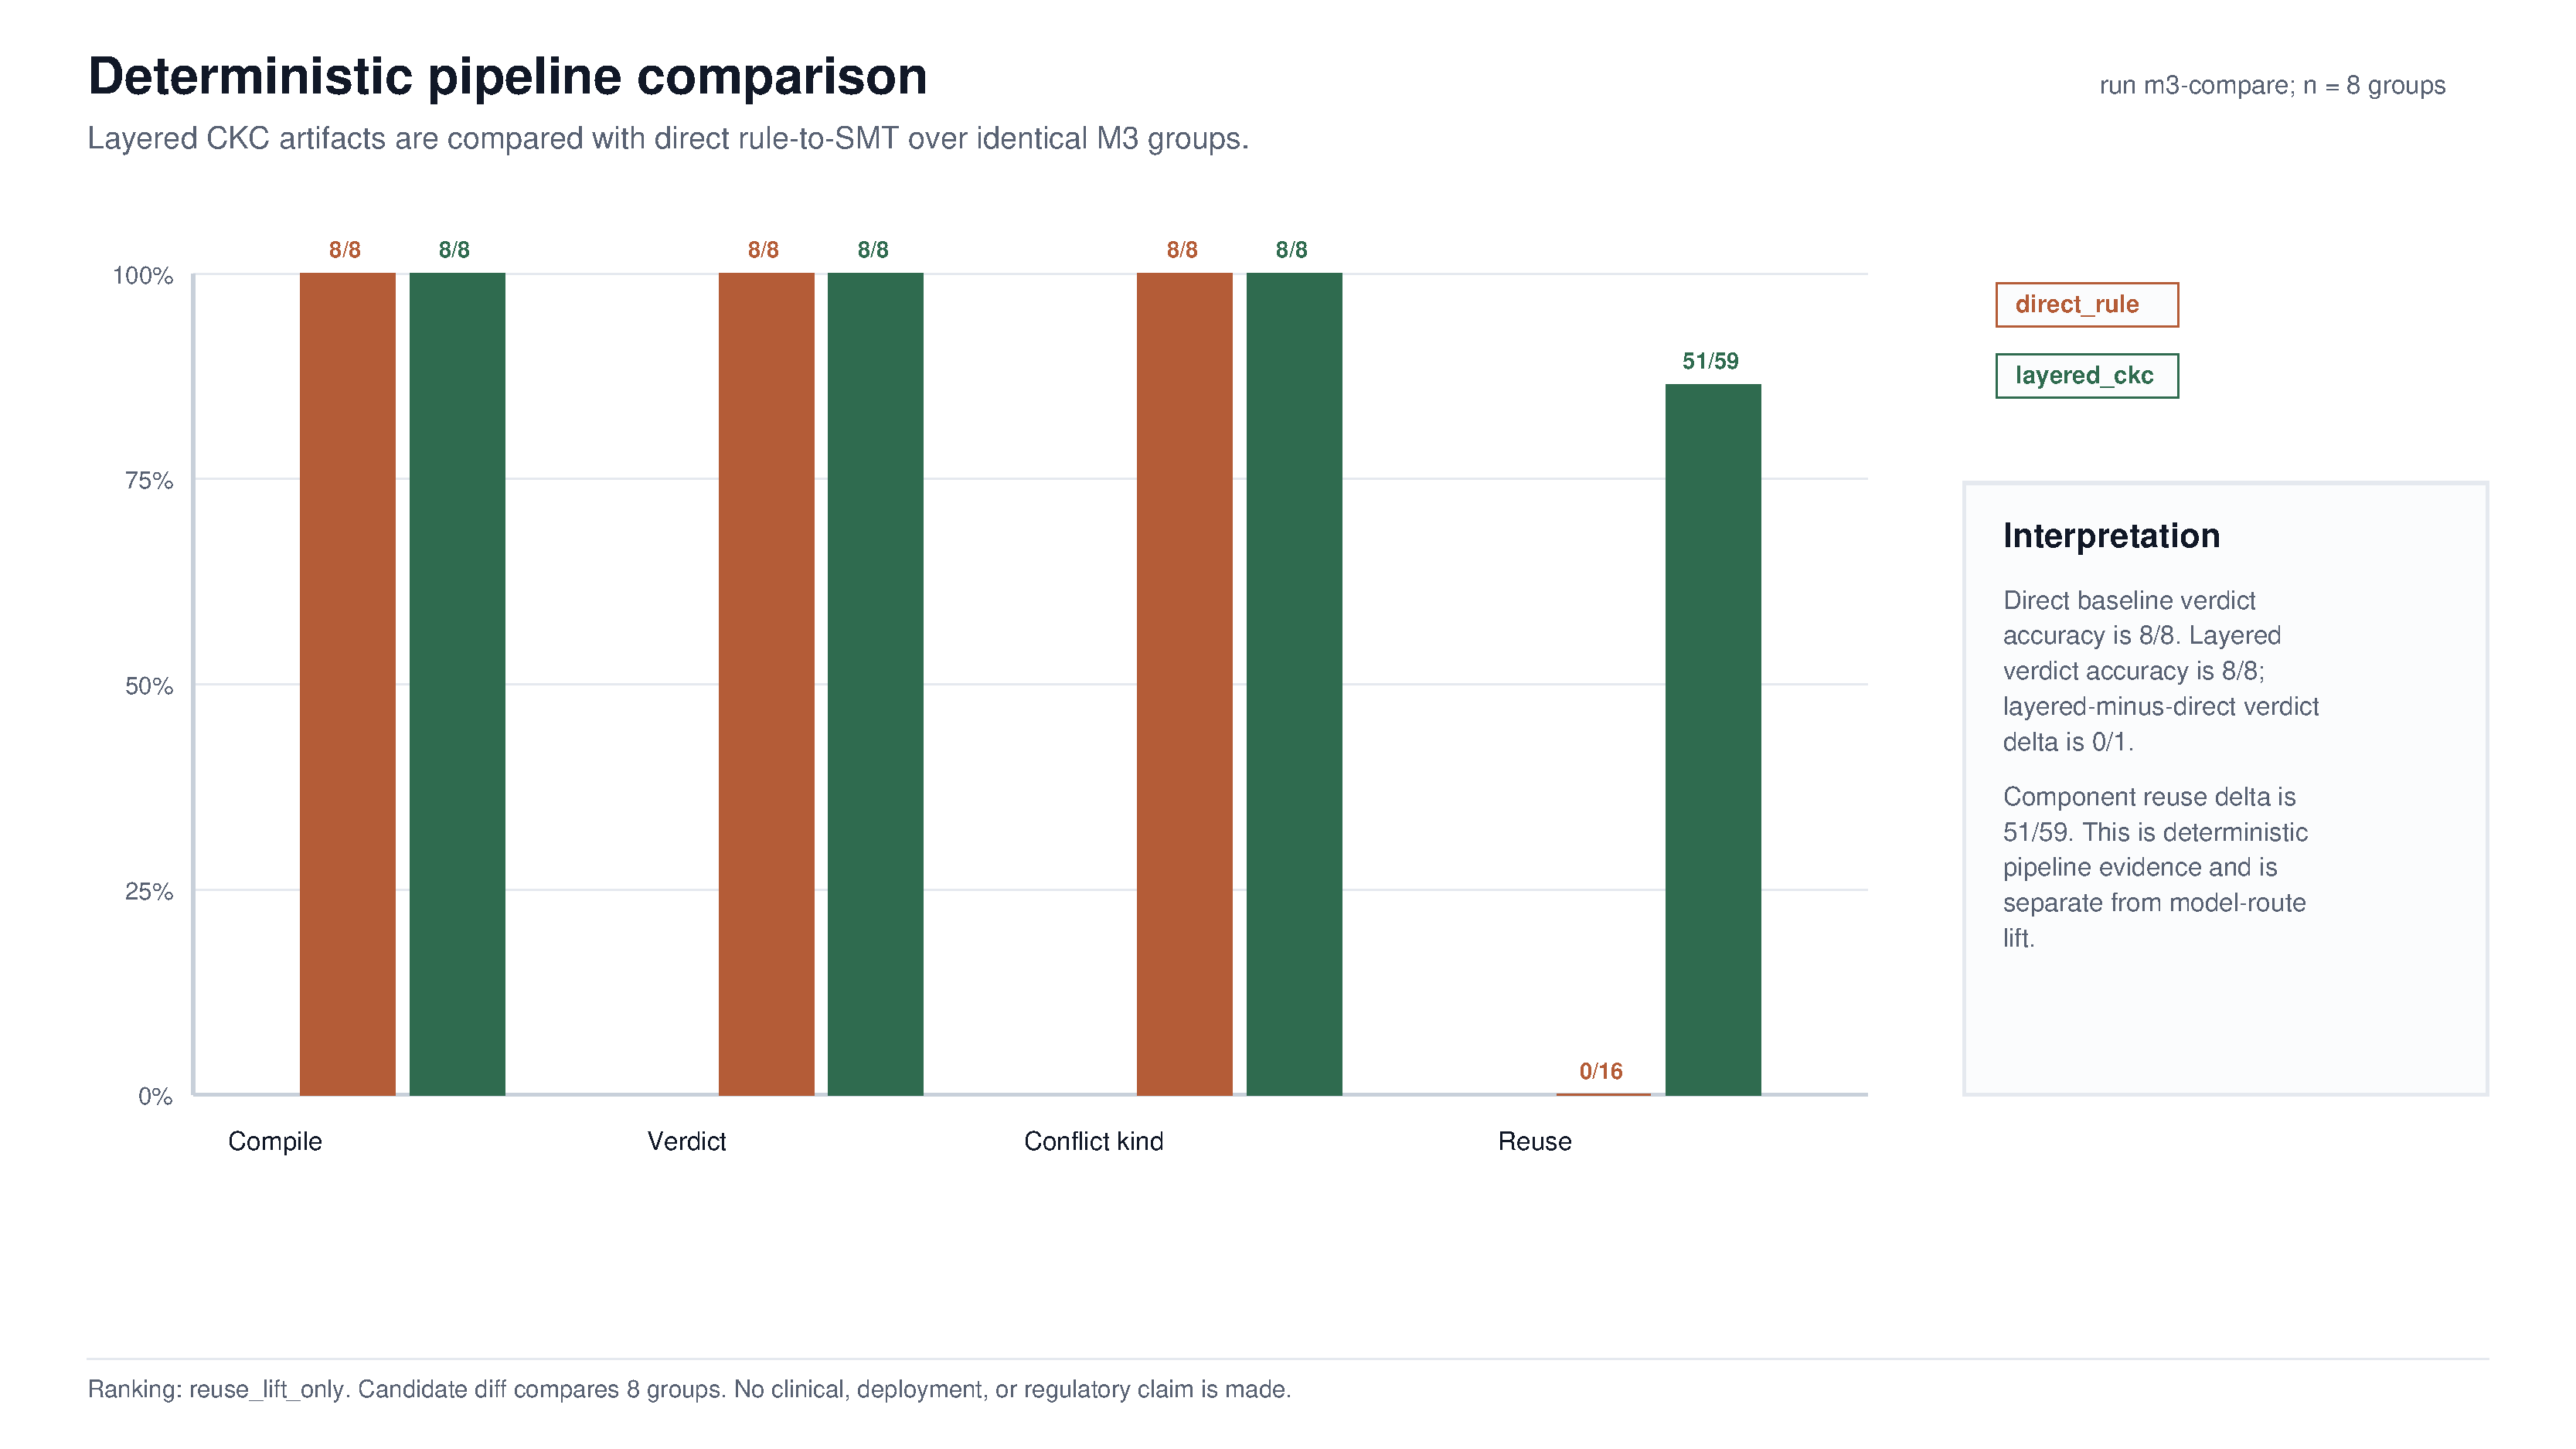
\includegraphics[width=\linewidth]{figures/manuscript/fig05_pipeline_comparison.pdf}
  \caption{Deterministic pipeline comparison. Direct rule-to-SMT is retained as baseline; profile lines show that the layered CKC pipeline matches verdict and conflict-kind accuracy in the current M3 comparison while component reuse is reported separately from model-route baseline deltas.}
  \label{fig:pipeline-comparison}
\end{figure}

\begin{figure}[t]
  \centering
  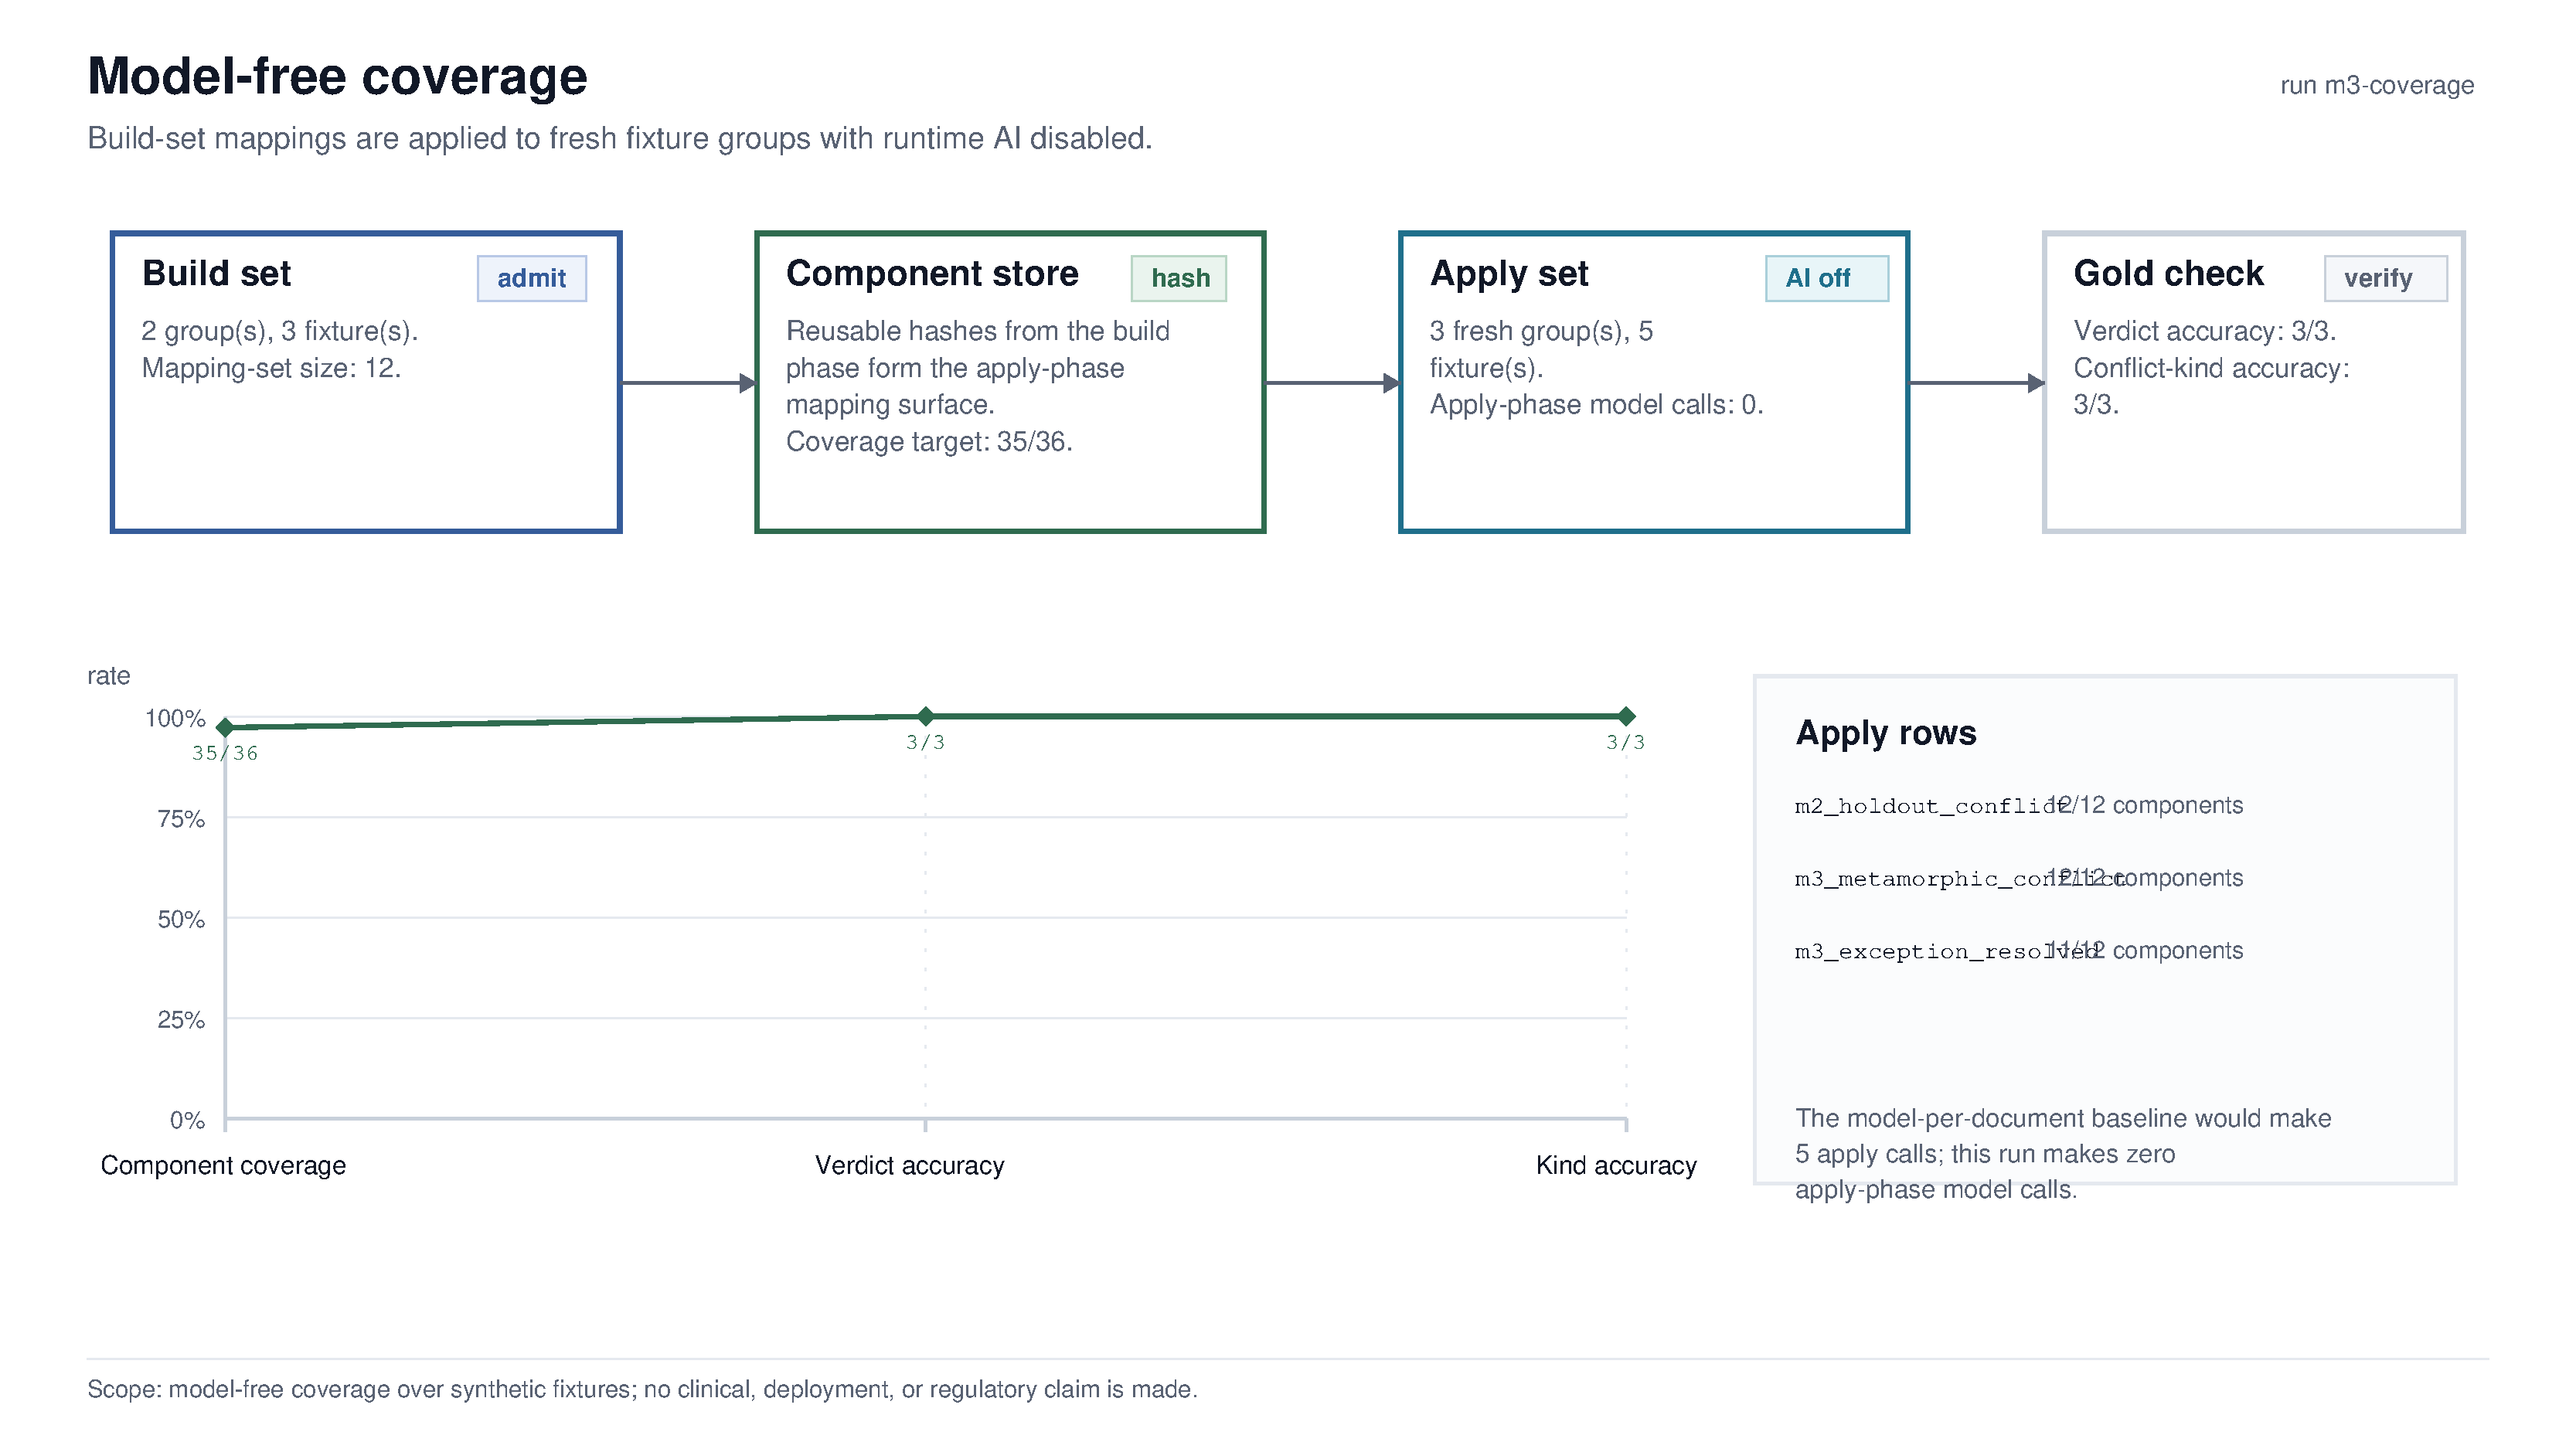
\includegraphics[width=\linewidth]{figures/manuscript/fig06_model_free_coverage.pdf}
  \caption{Model-free coverage. Build-set mappings are applied to fresh synthetic fixture groups with runtime AI disabled; component coverage, verdict accuracy, and zero apply-phase model calls are reported as exact ratios/counts.}
  \label{fig:model-free-coverage}
\end{figure}
 or copy individual figure blocks.

\begin{figure}[t]
  \centering
  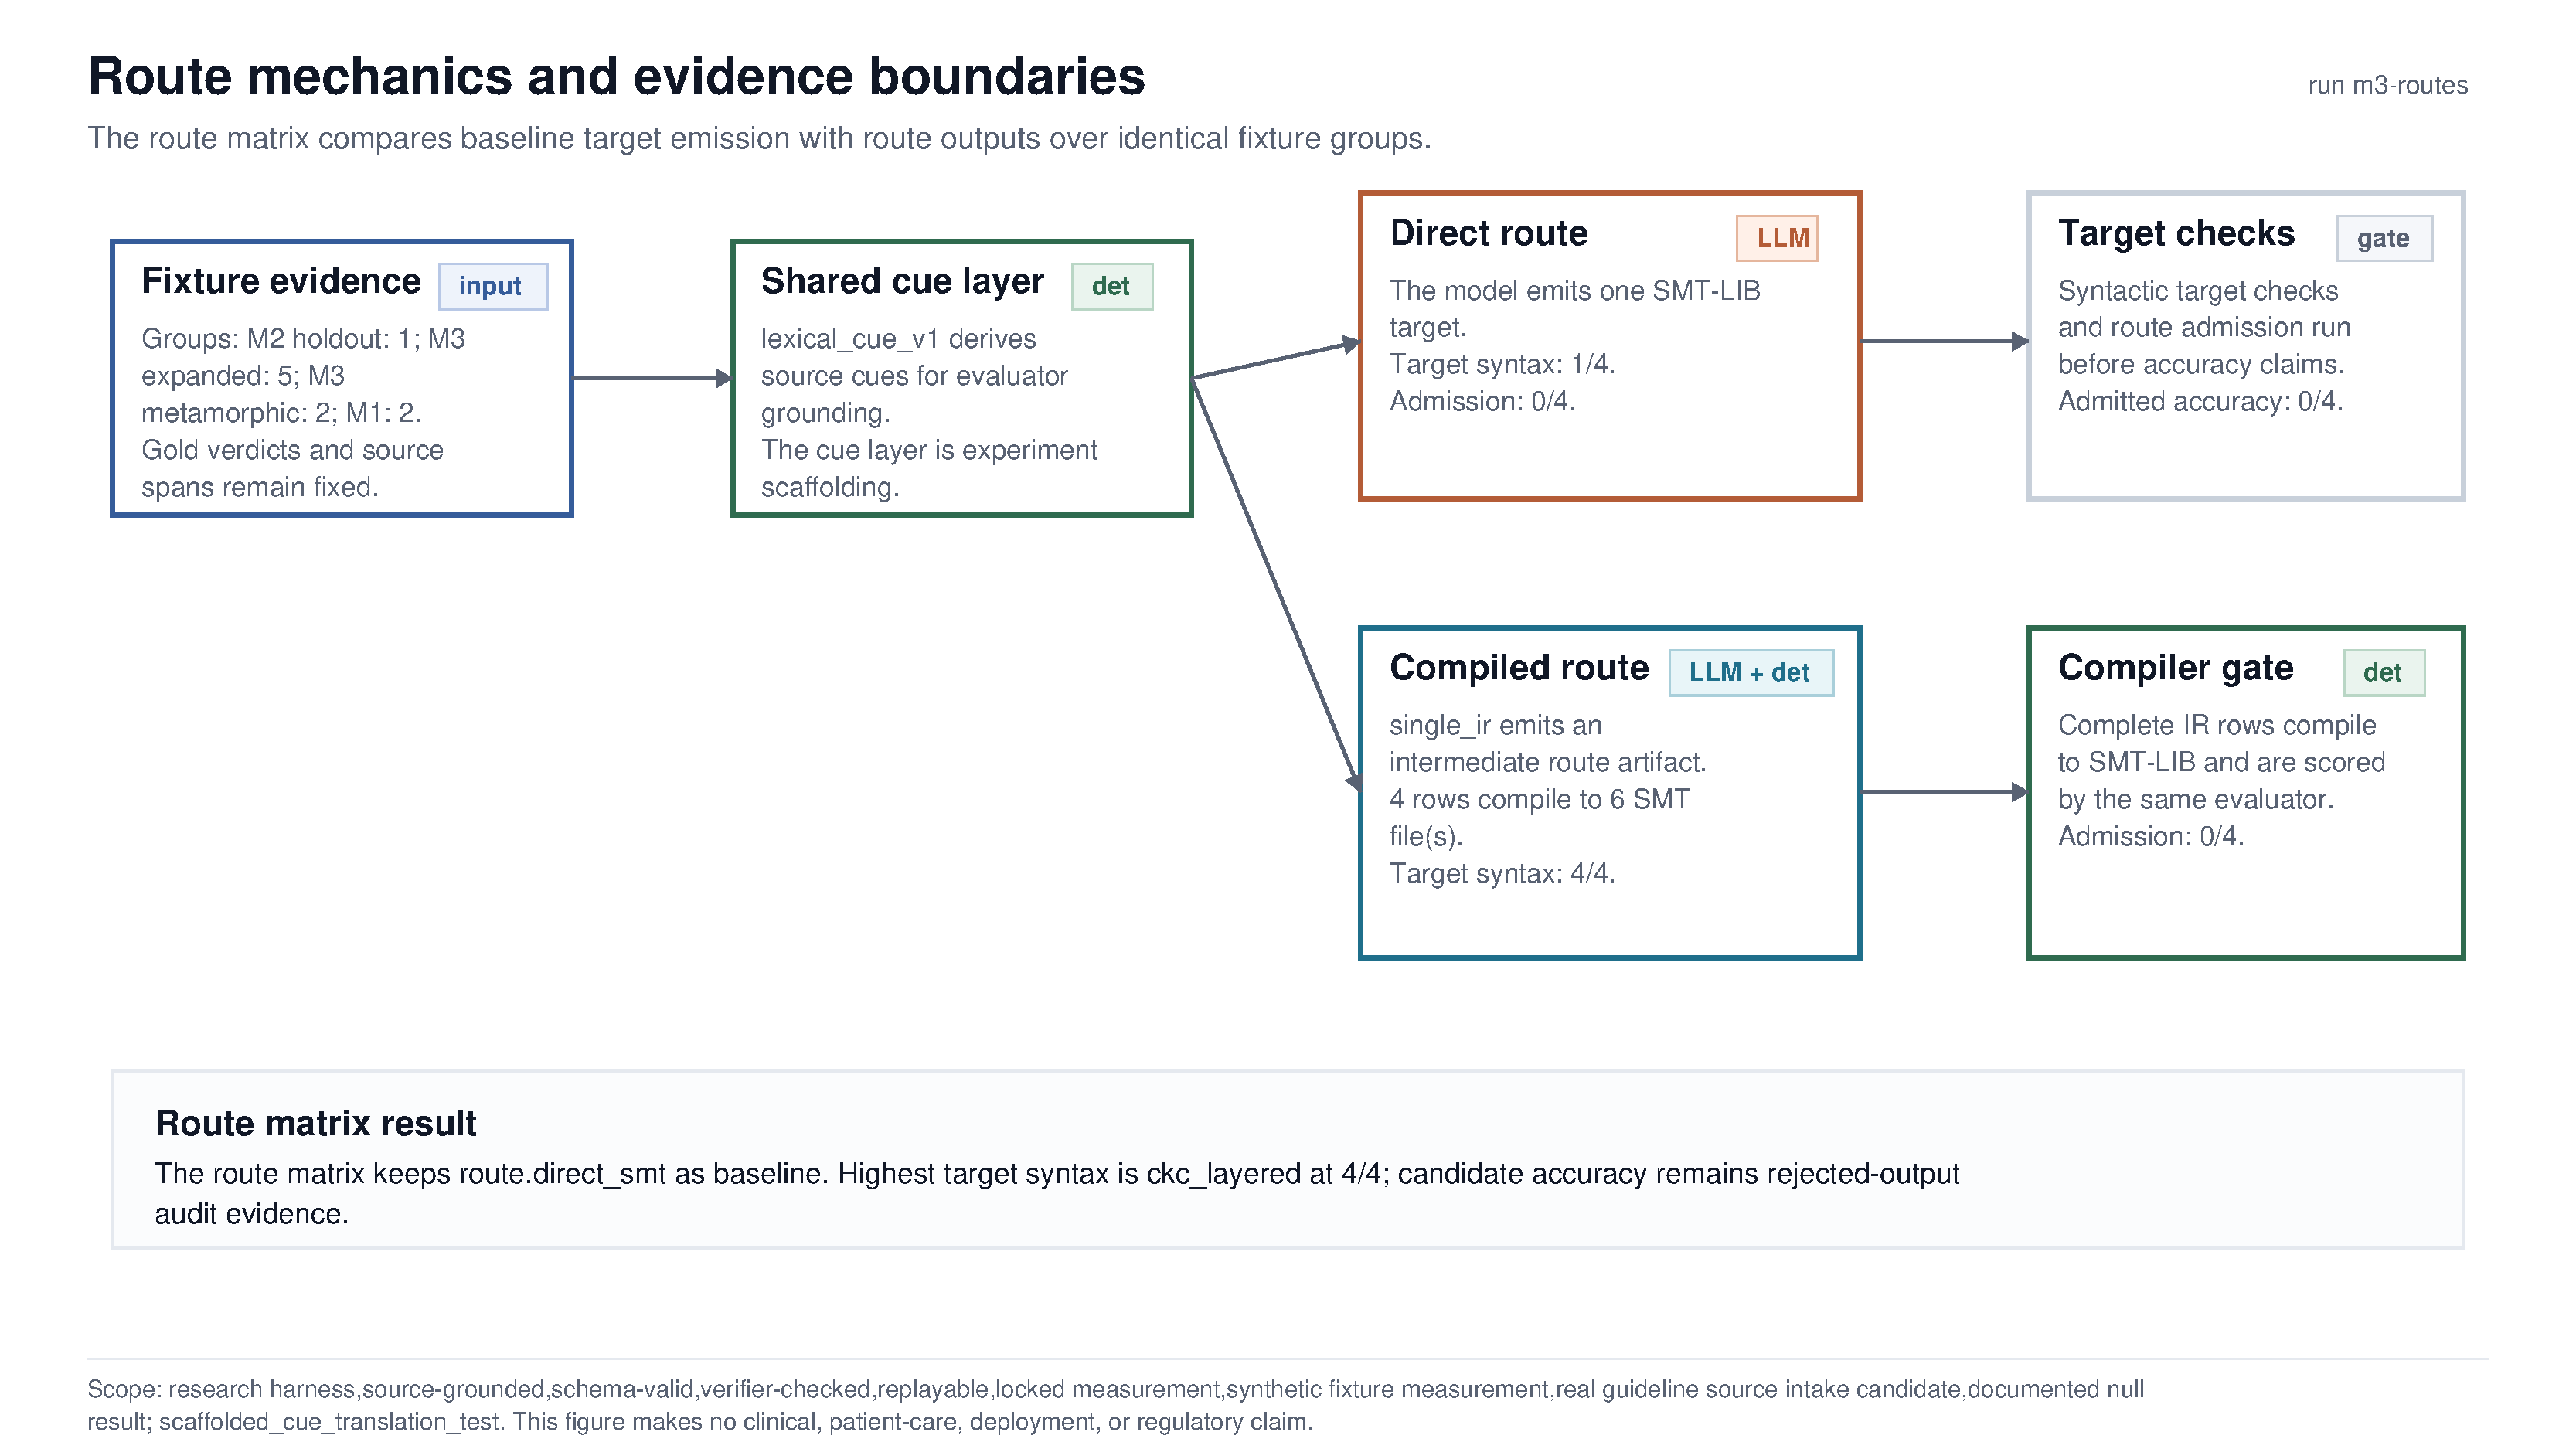
\includegraphics[width=\linewidth]{figures/manuscript/fig01_route_mechanics.pdf}
  \caption{Route mechanics. Implemented routes consume the same fixture groups and are scored by the same evaluator; the current run shows a target-syntax baseline delta only, not an admitted-verdict baseline delta.}
  \label{fig:route-mechanics}
\end{figure}

\begin{figure}[t]
  \centering
  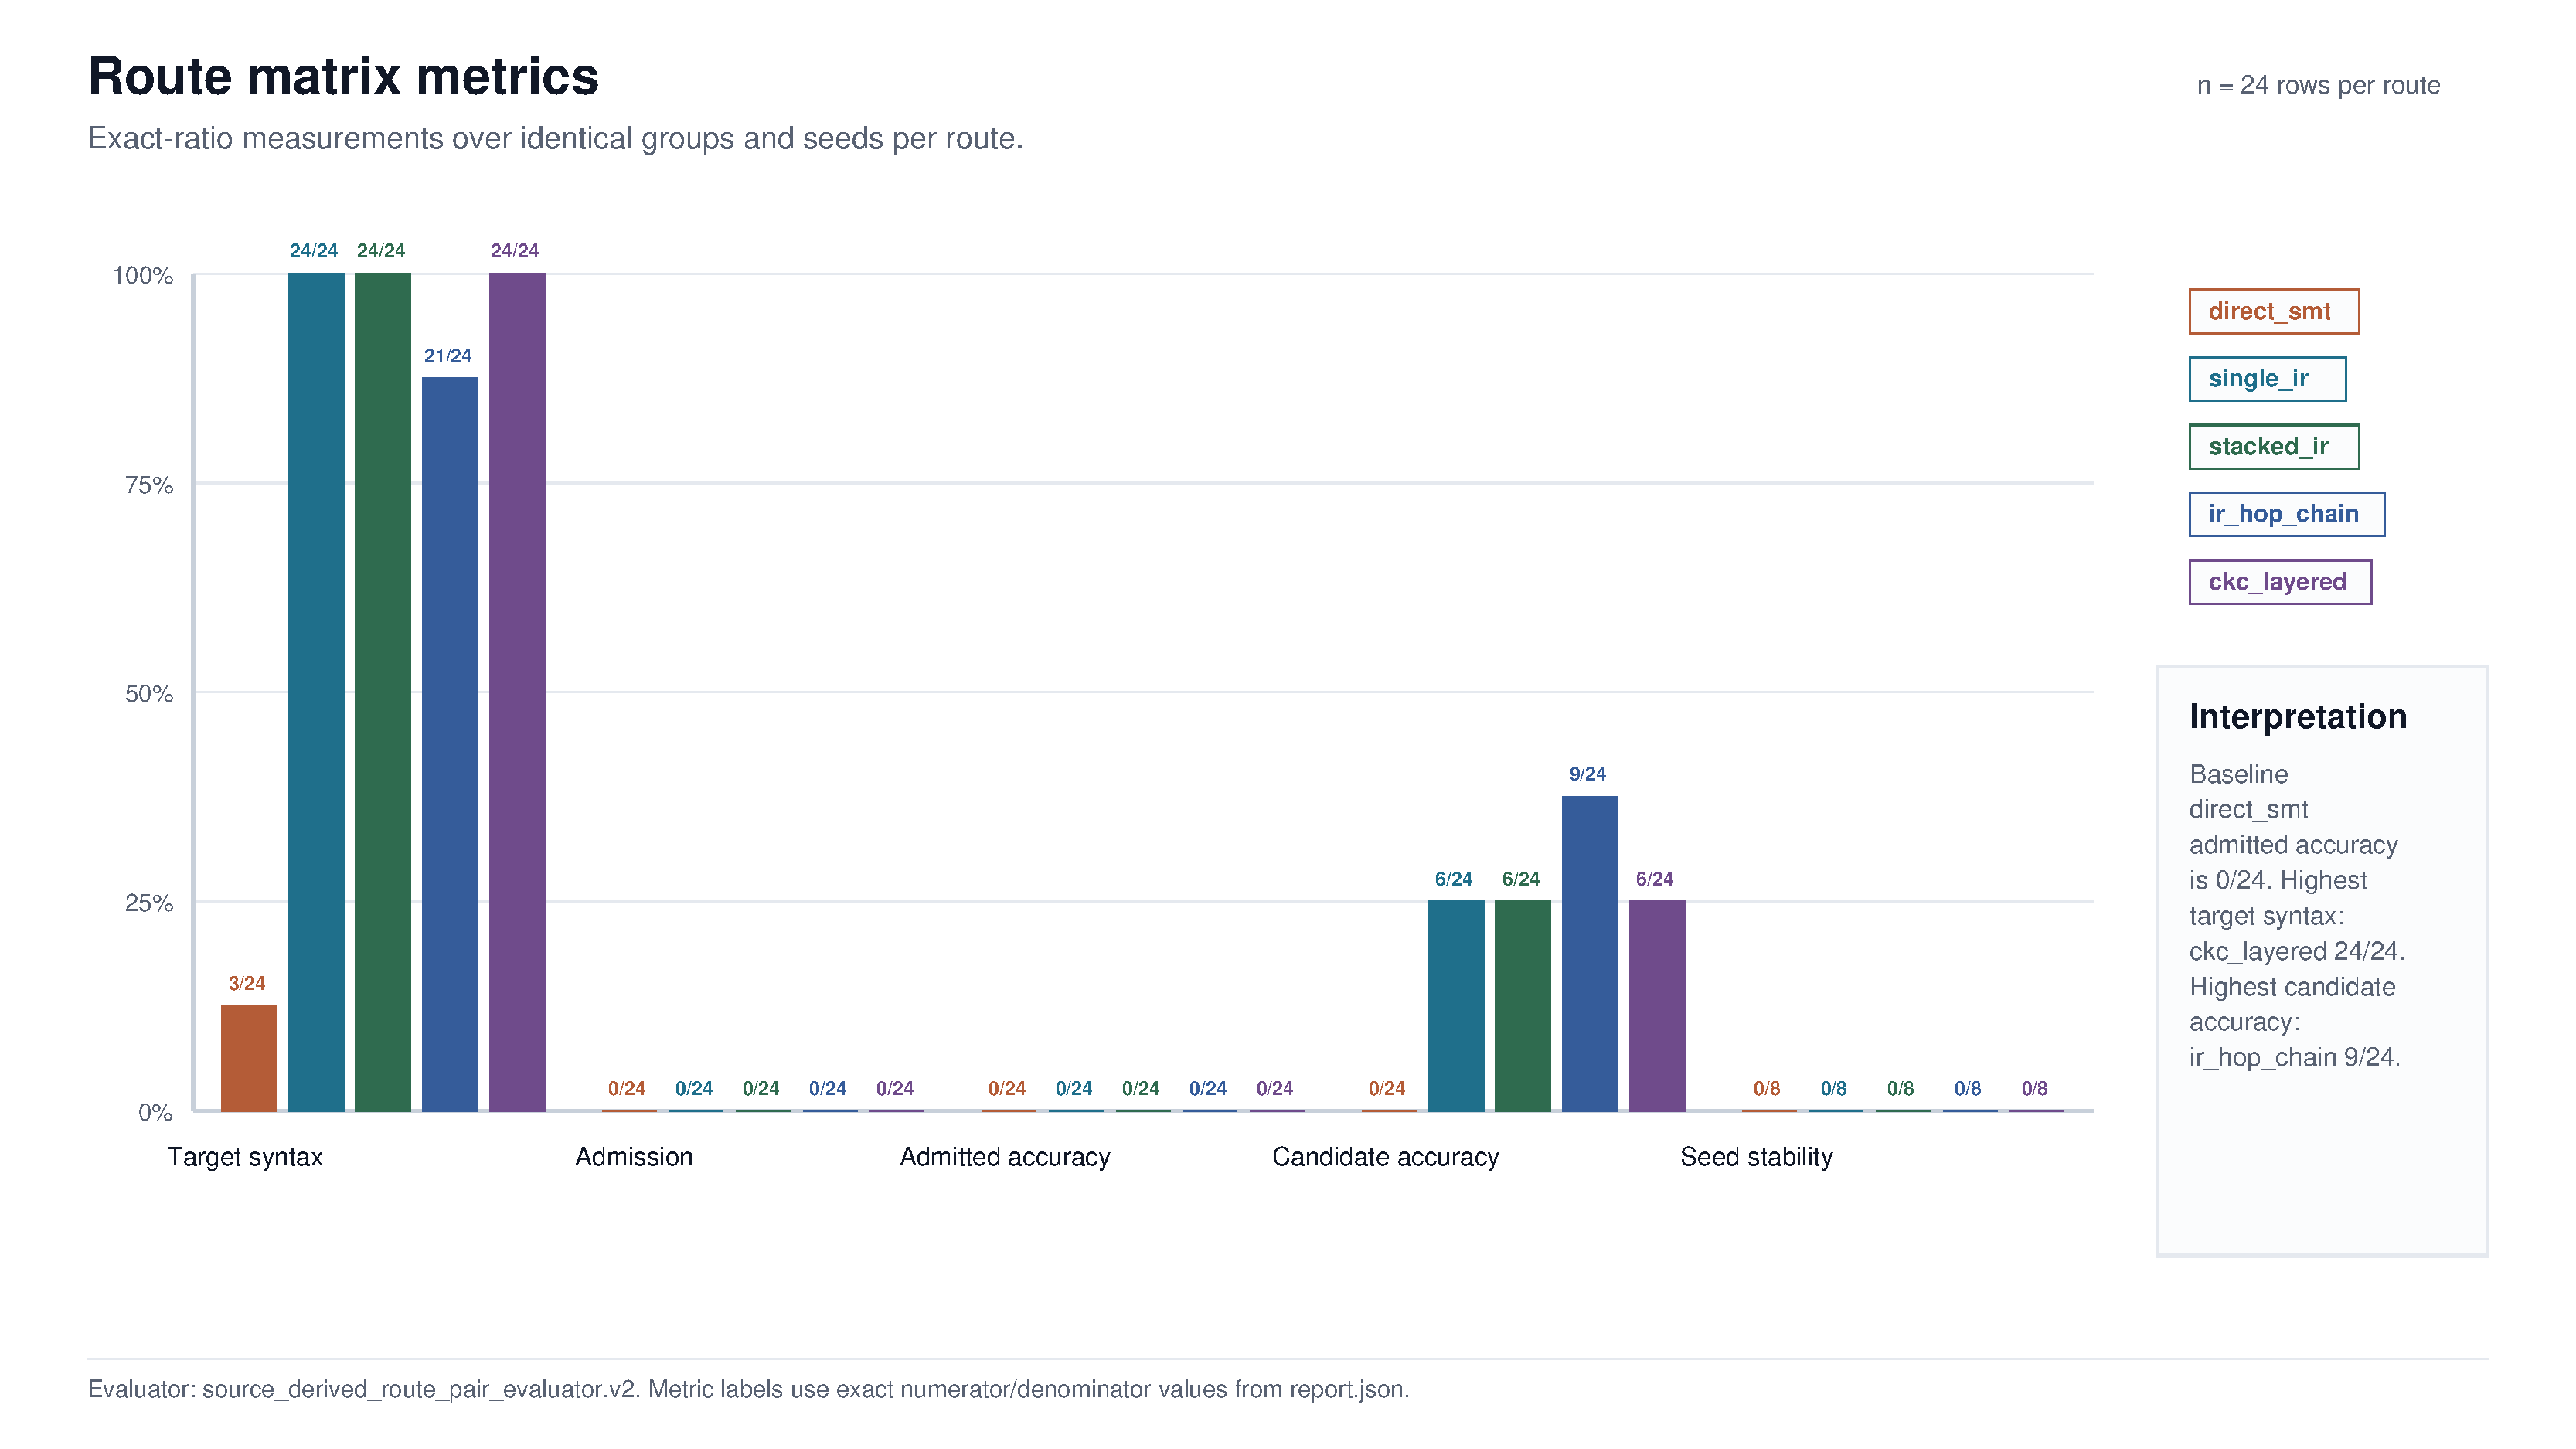
\includegraphics[width=\linewidth]{figures/manuscript/fig02_route_metrics.pdf}
  \caption{Route metrics from the current run, shown as exact-ratio profile lines over the route matrix with direct SMT retained as baseline. Candidate verdict accuracy is rejected-output audit evidence, not admitted baseline improvement.}
  \label{fig:route-metrics}
\end{figure}

\begin{figure}[t]
  \centering
  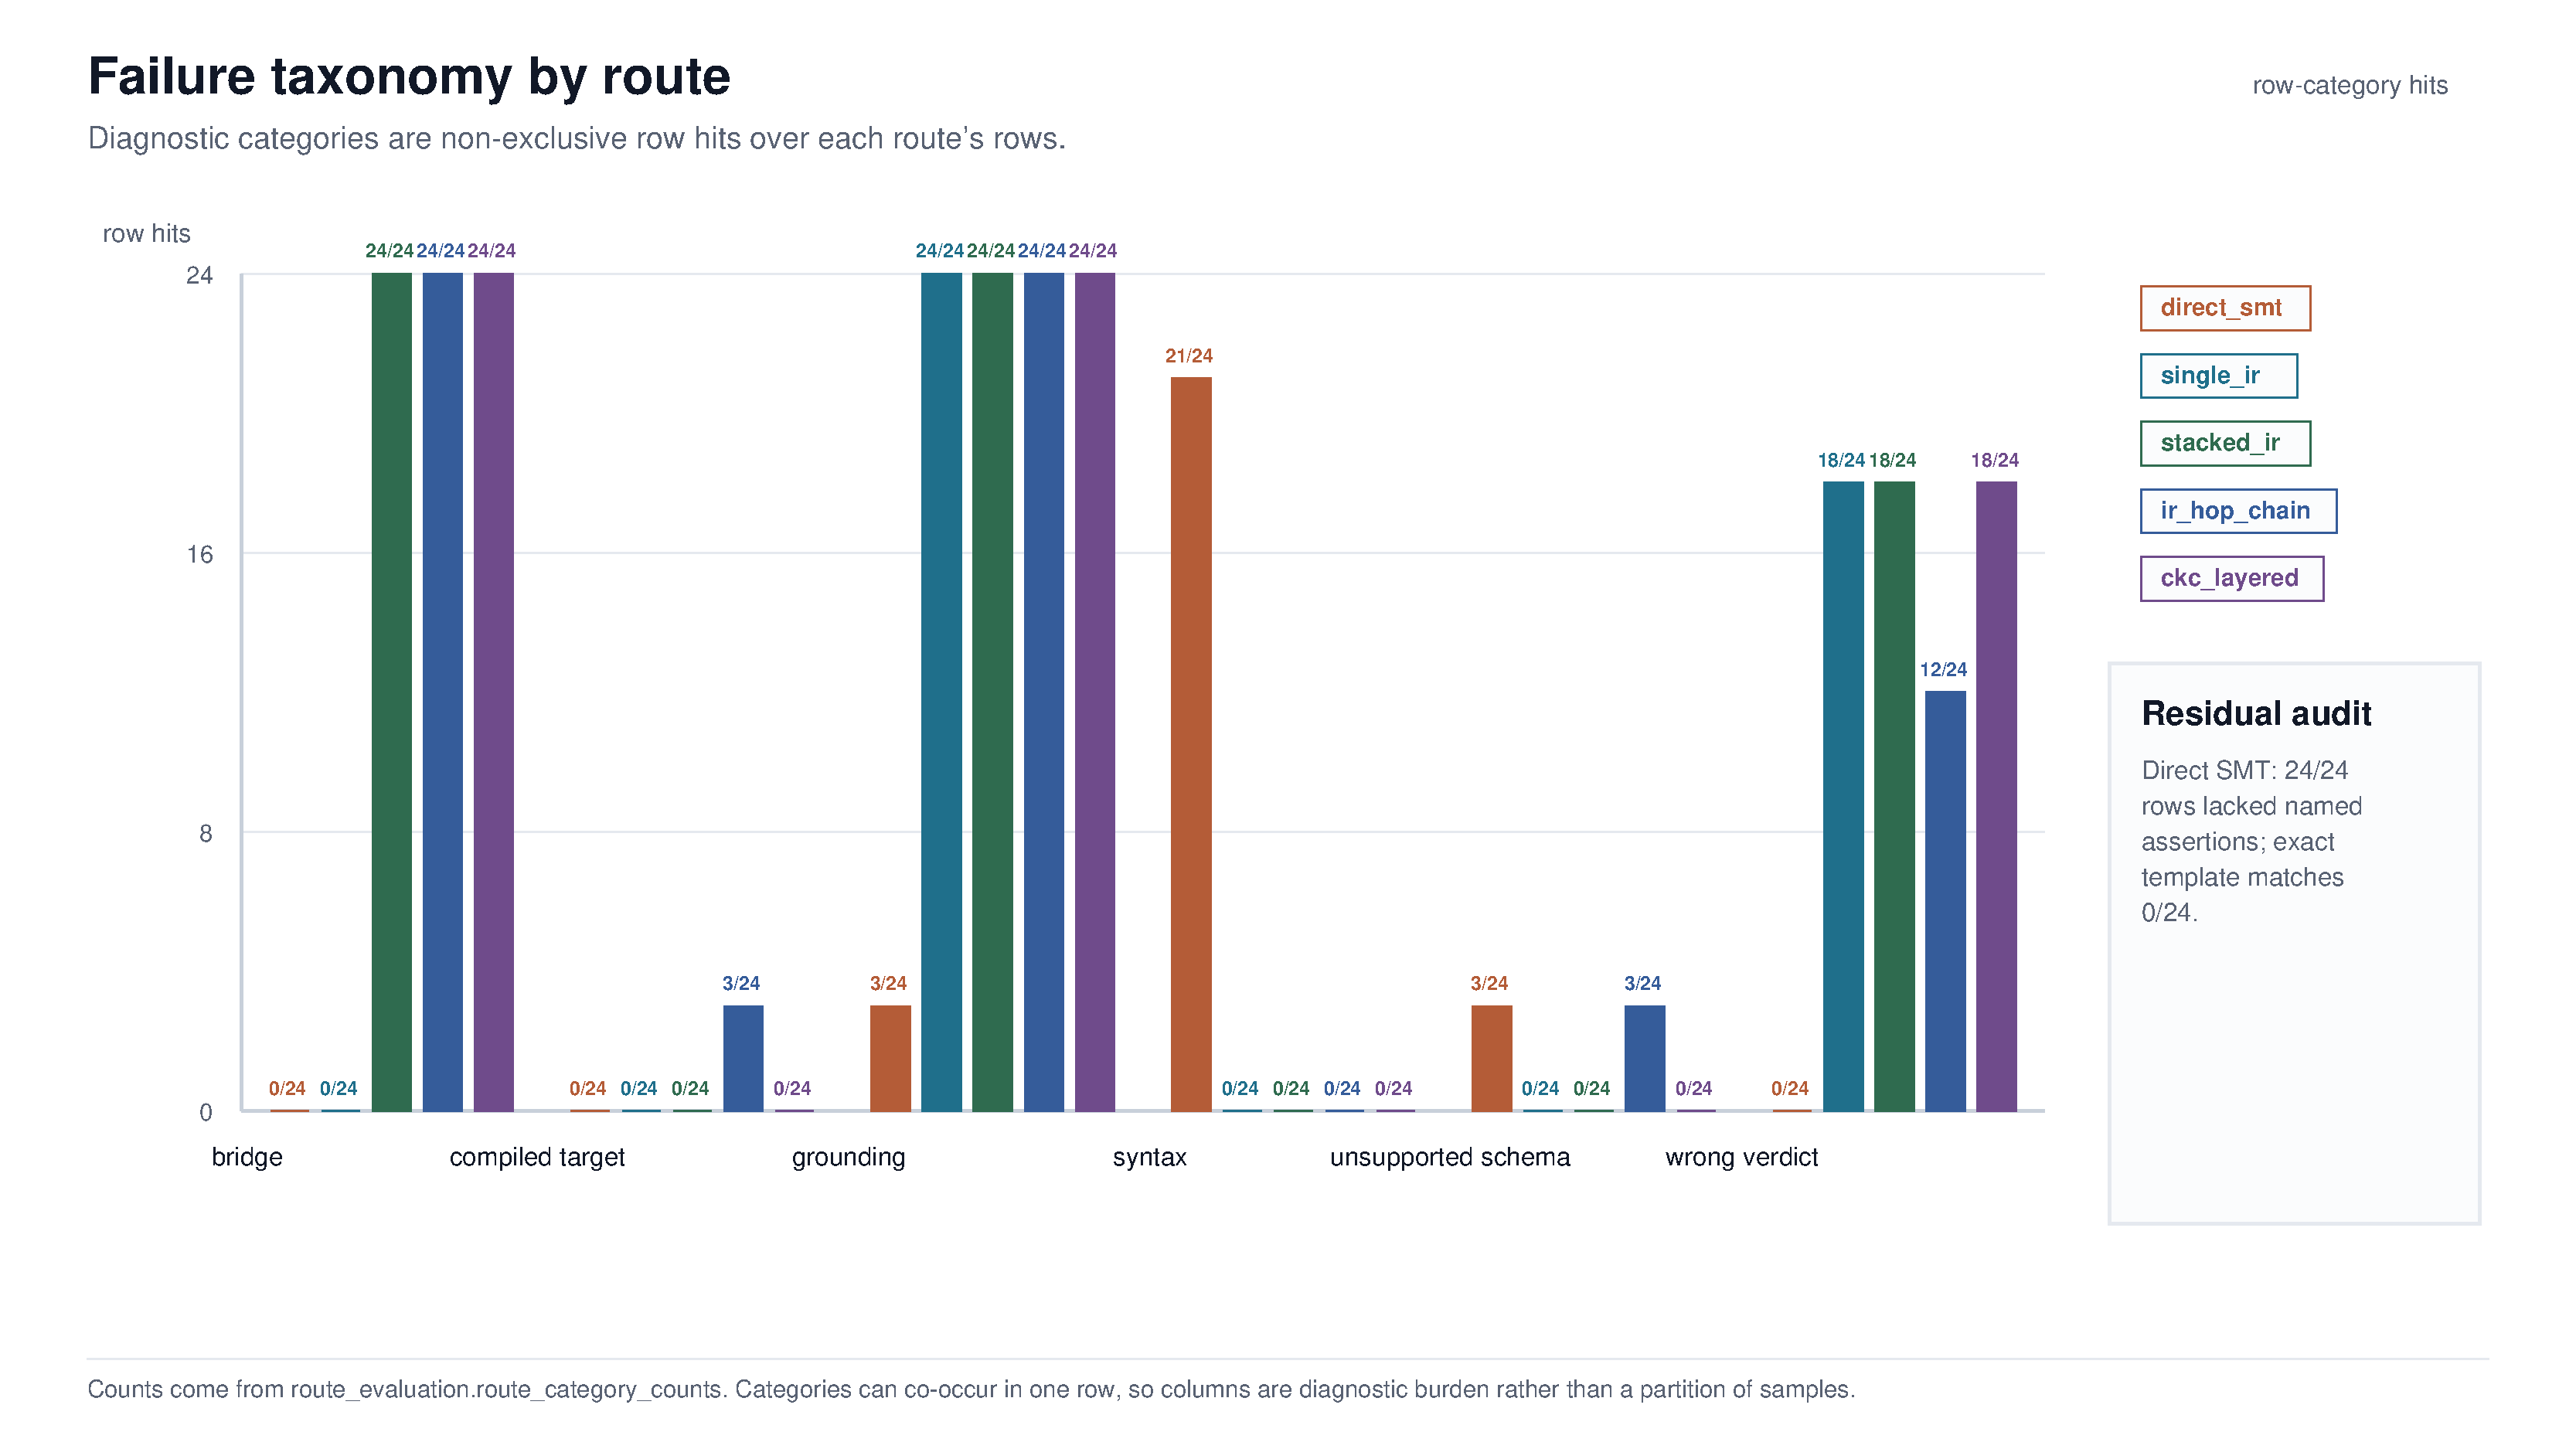
\includegraphics[width=\linewidth]{figures/manuscript/fig03_failure_taxonomy.pdf}
  \caption{Diagnostic row-category hits are shown as route profiles over the route matrix. Categories can co-occur, so profiles show diagnostic burden rather than a partition of samples.}
  \label{fig:failure-taxonomy}
\end{figure}

\begin{figure}[t]
  \centering
  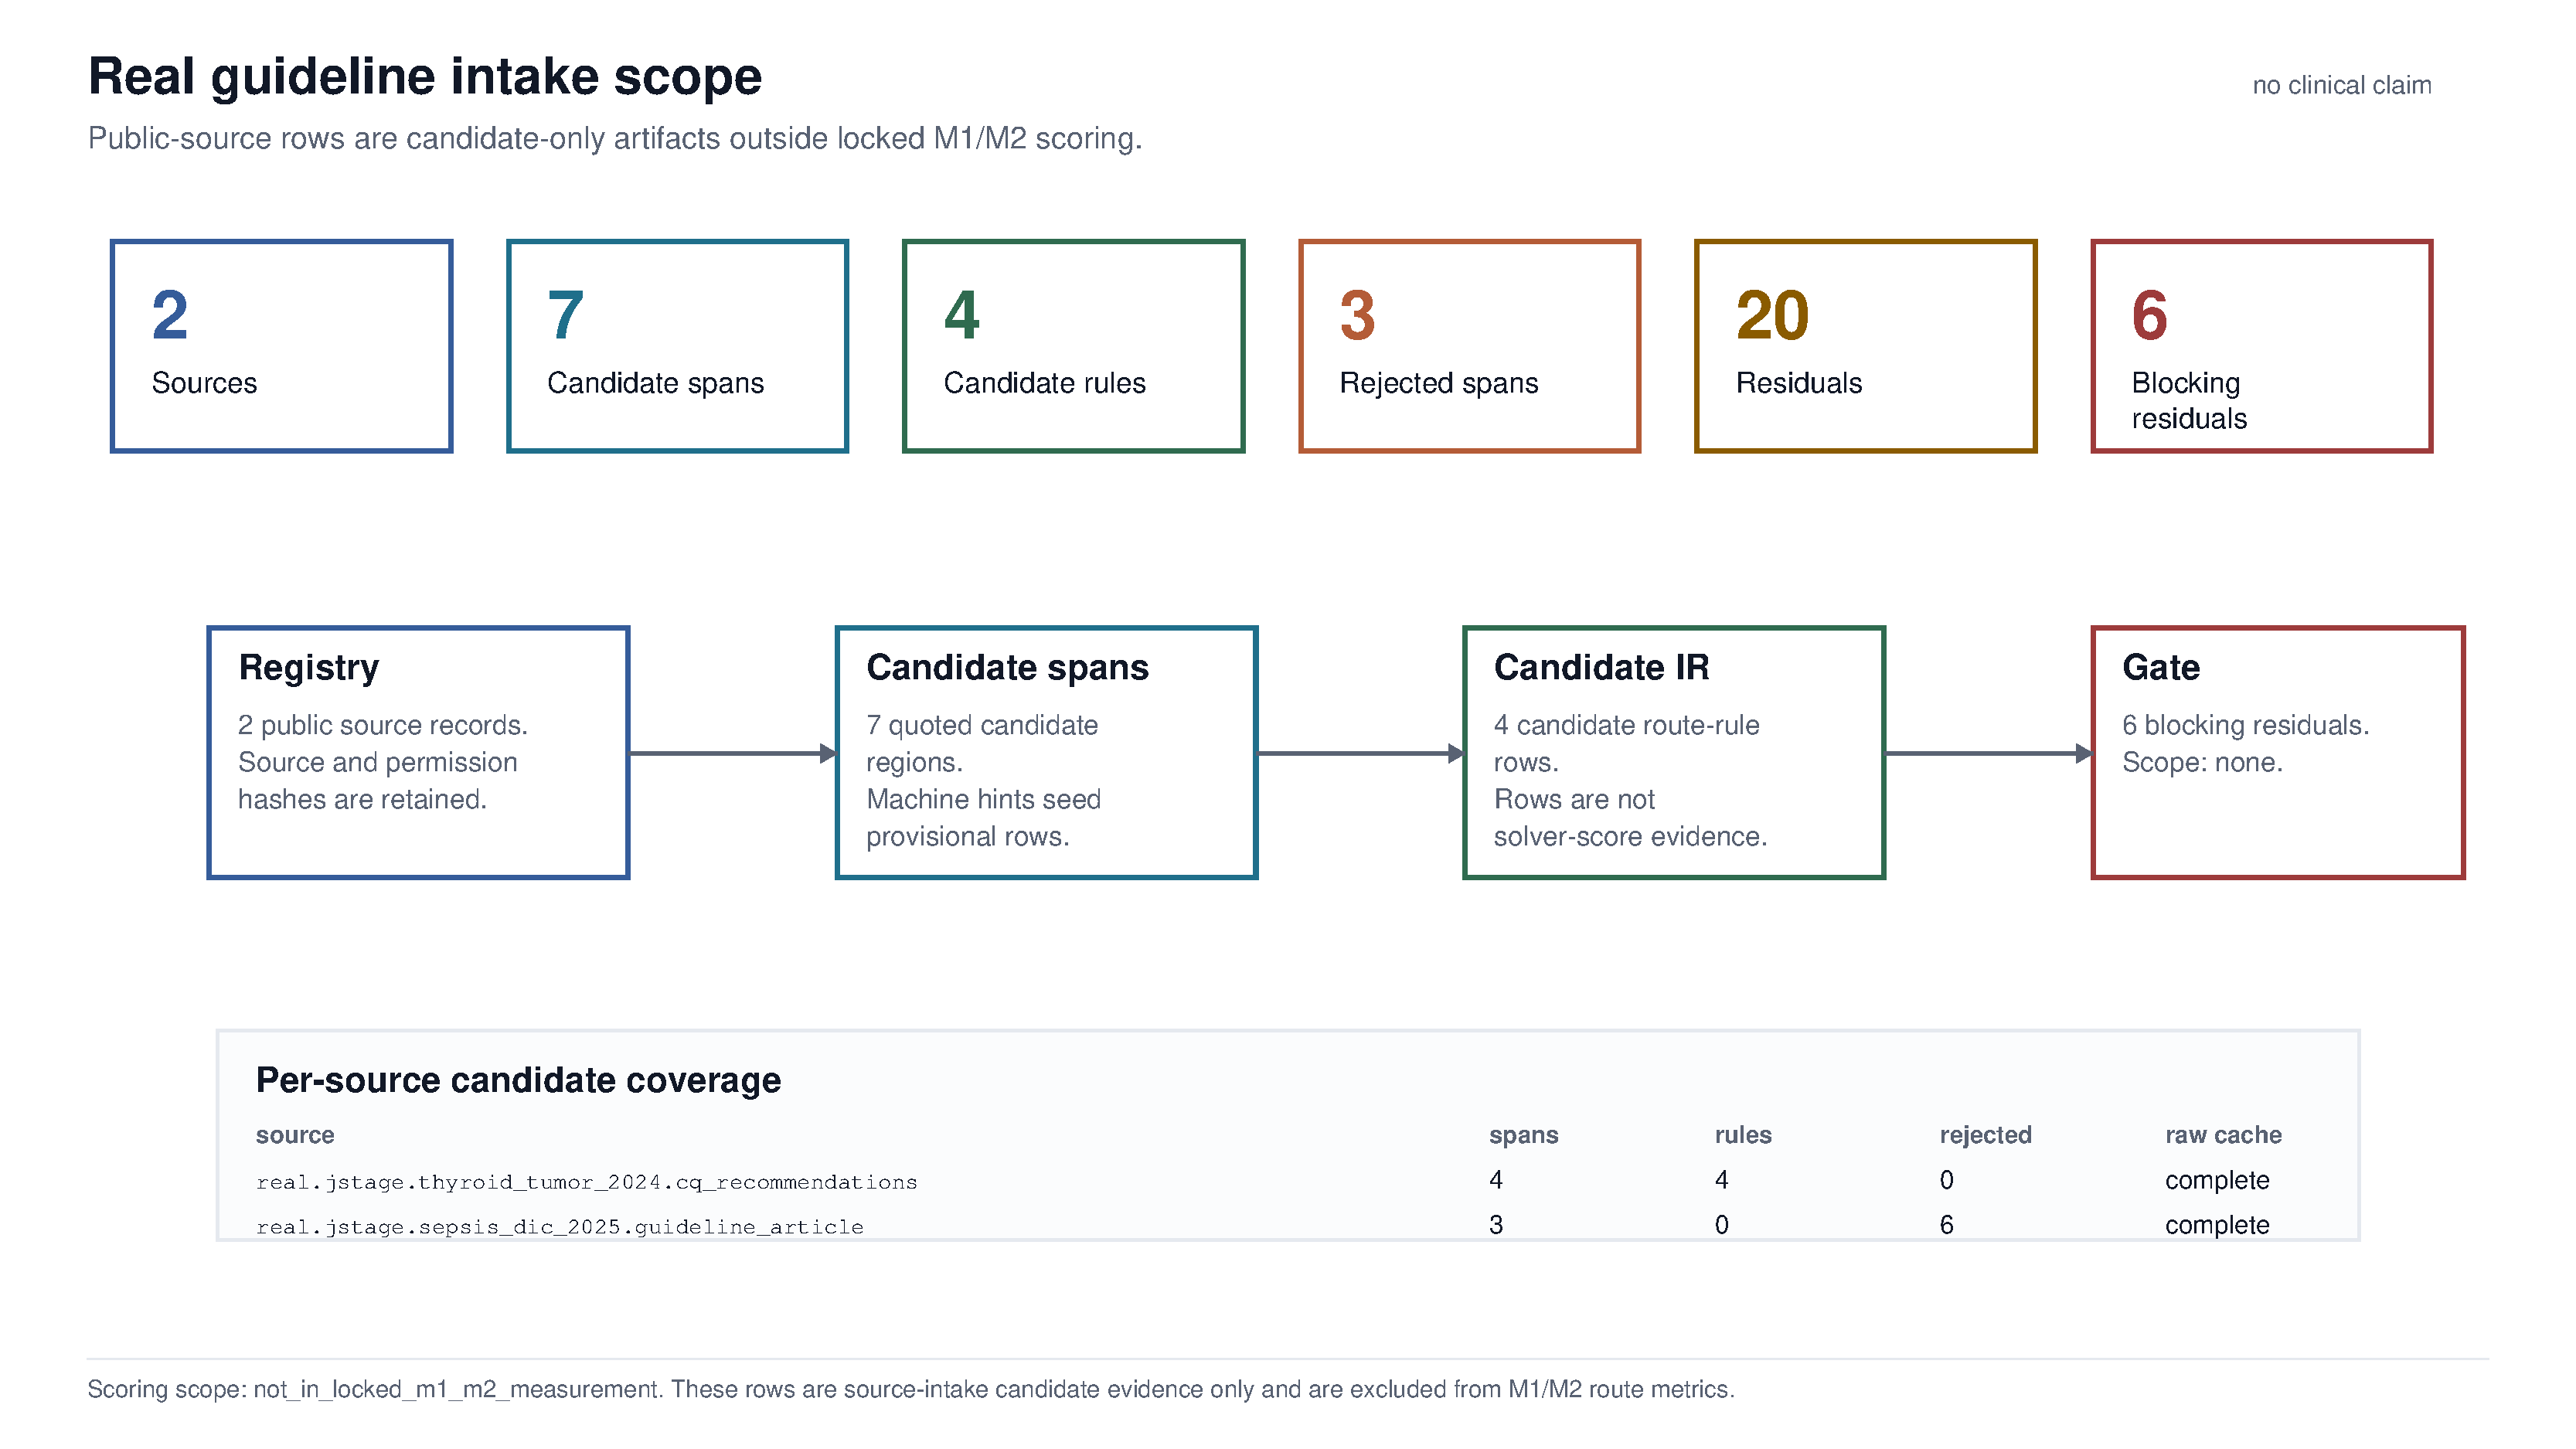
\includegraphics[width=\linewidth]{figures/manuscript/fig04_real_source_intake.pdf}
  \caption{Real Japanese guideline sources are represented as candidate-only source-intake artifacts with source and permission hashes, but they remain outside locked M1/M2 scoring and carry no clinical claim.}
  \label{fig:real-source-intake}
\end{figure}

\begin{figure}[t]
  \centering
  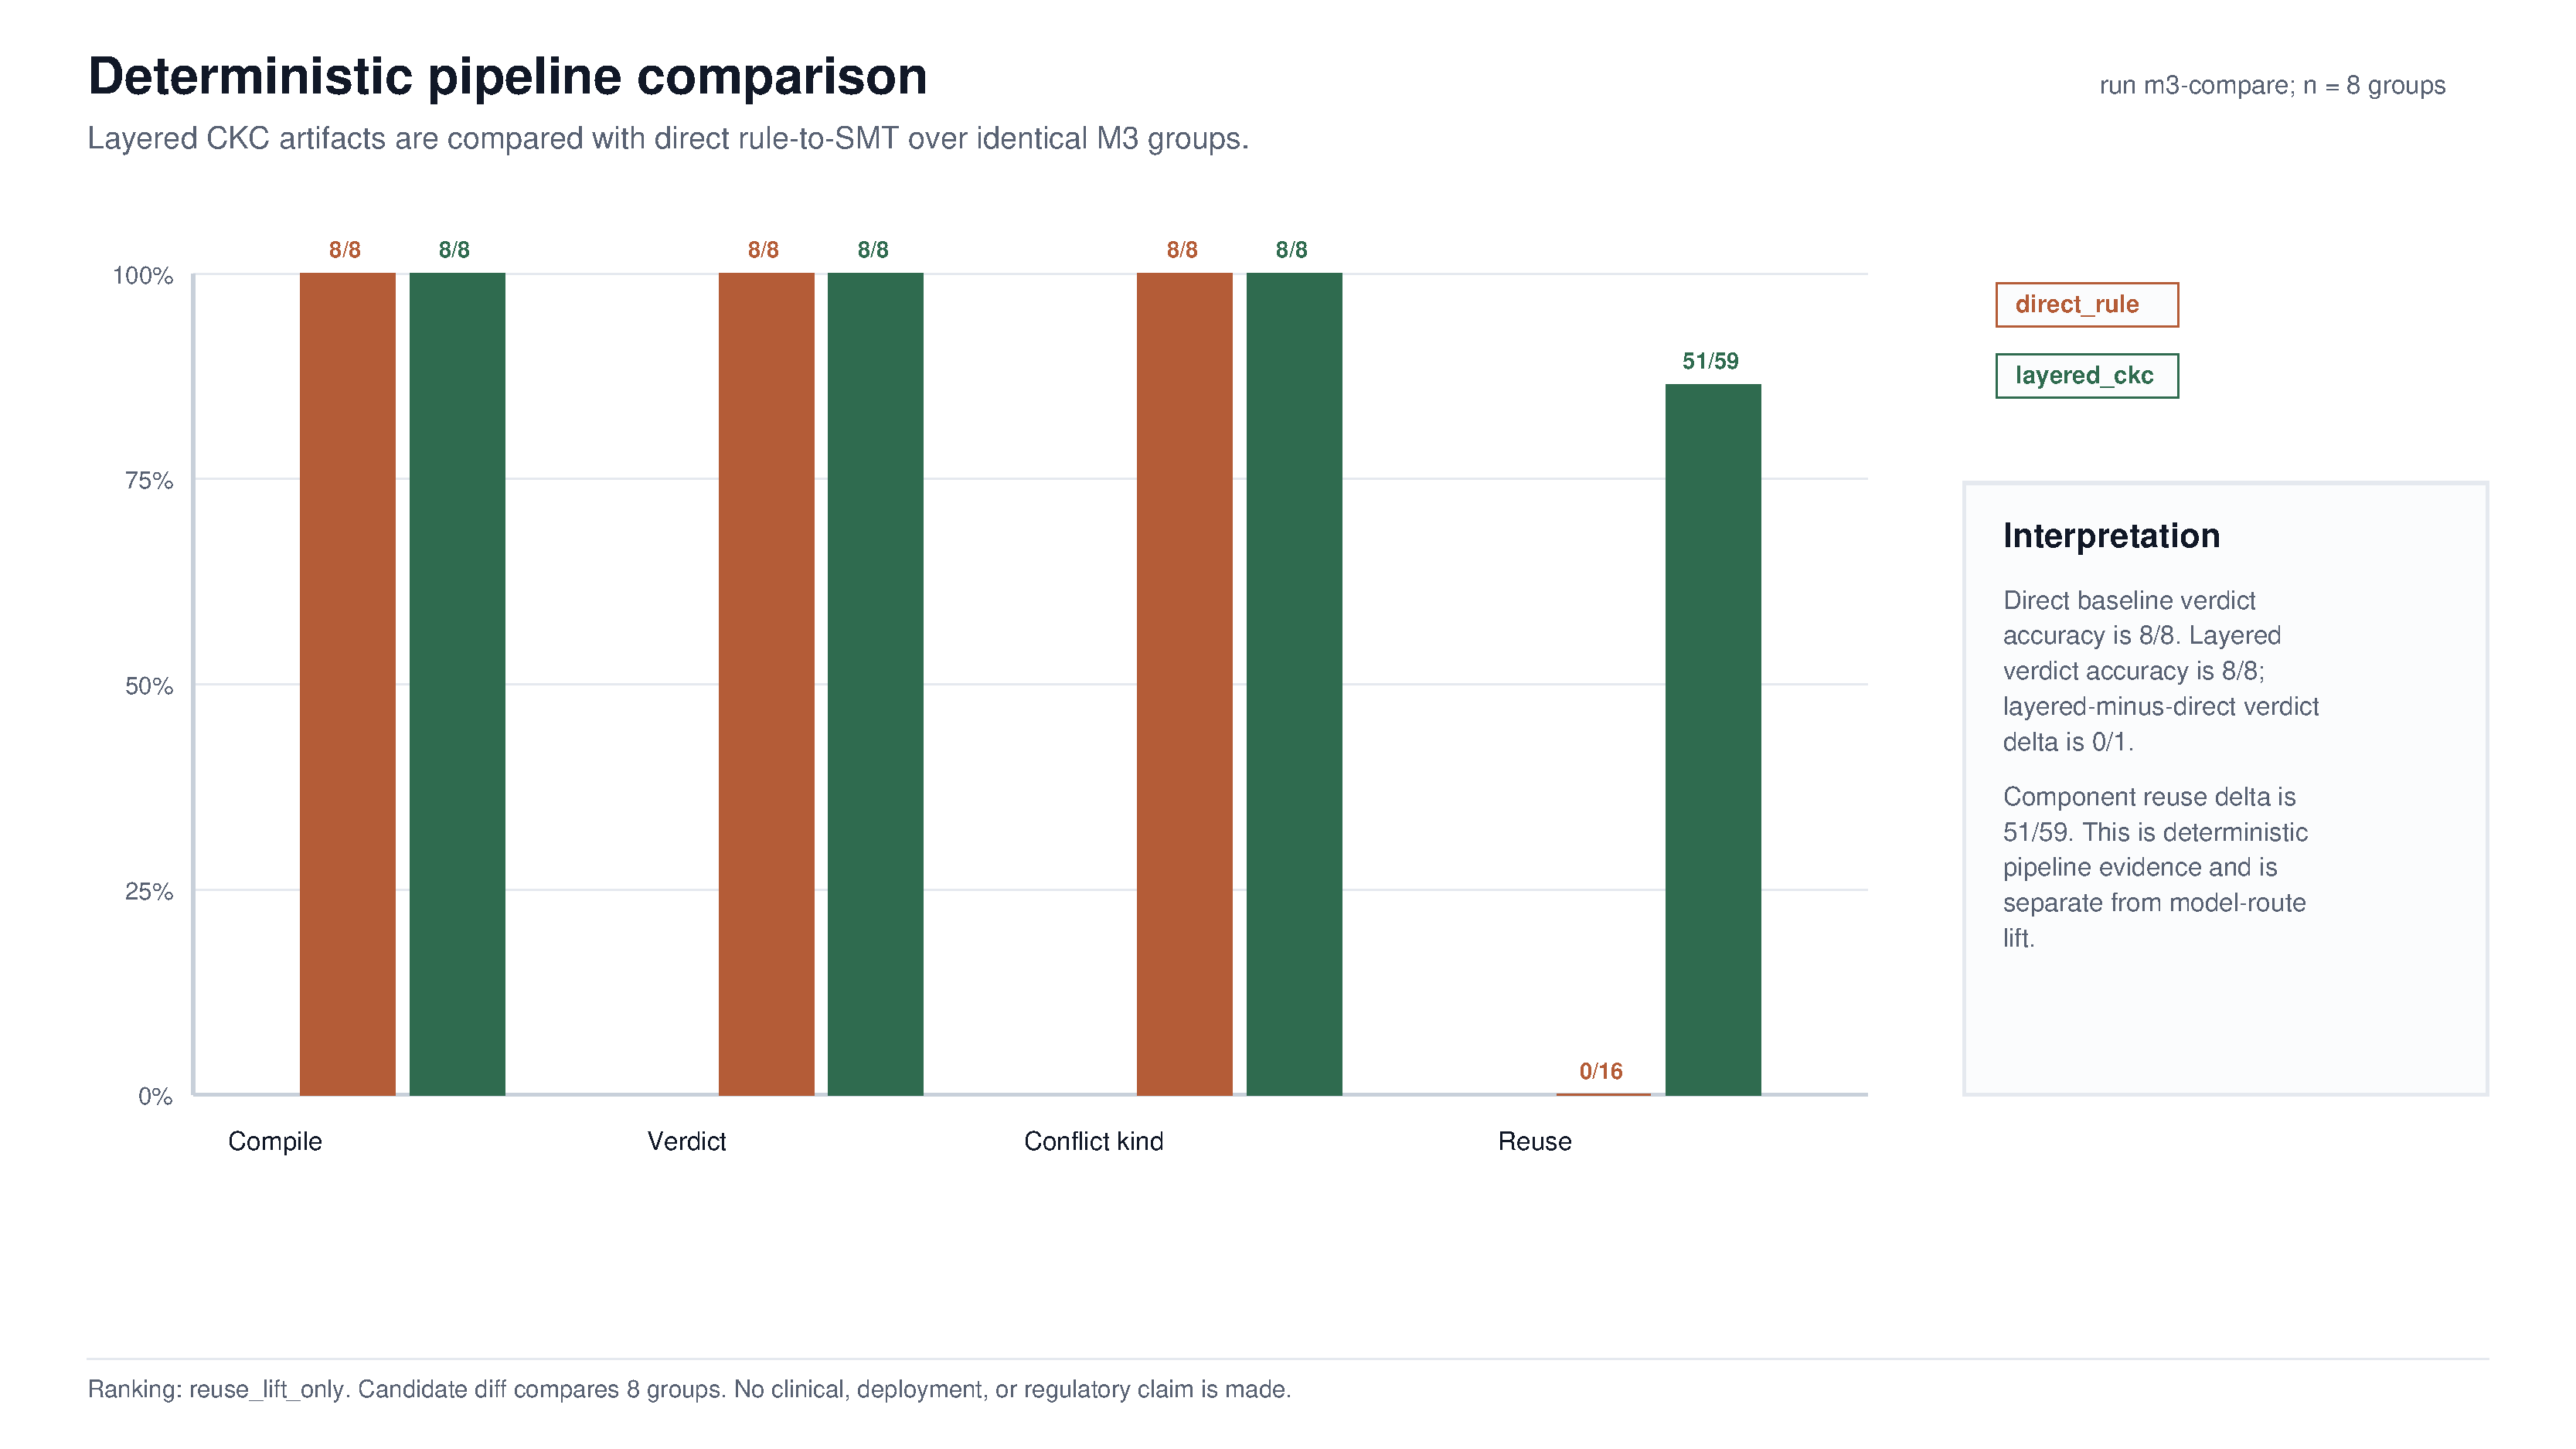
\includegraphics[width=\linewidth]{figures/manuscript/fig05_pipeline_comparison.pdf}
  \caption{Deterministic pipeline comparison. Direct rule-to-SMT is retained as baseline; profile lines show that the layered CKC pipeline matches verdict and conflict-kind accuracy in the current M3 comparison while component reuse is reported separately from model-route baseline deltas.}
  \label{fig:pipeline-comparison}
\end{figure}

\begin{figure}[t]
  \centering
  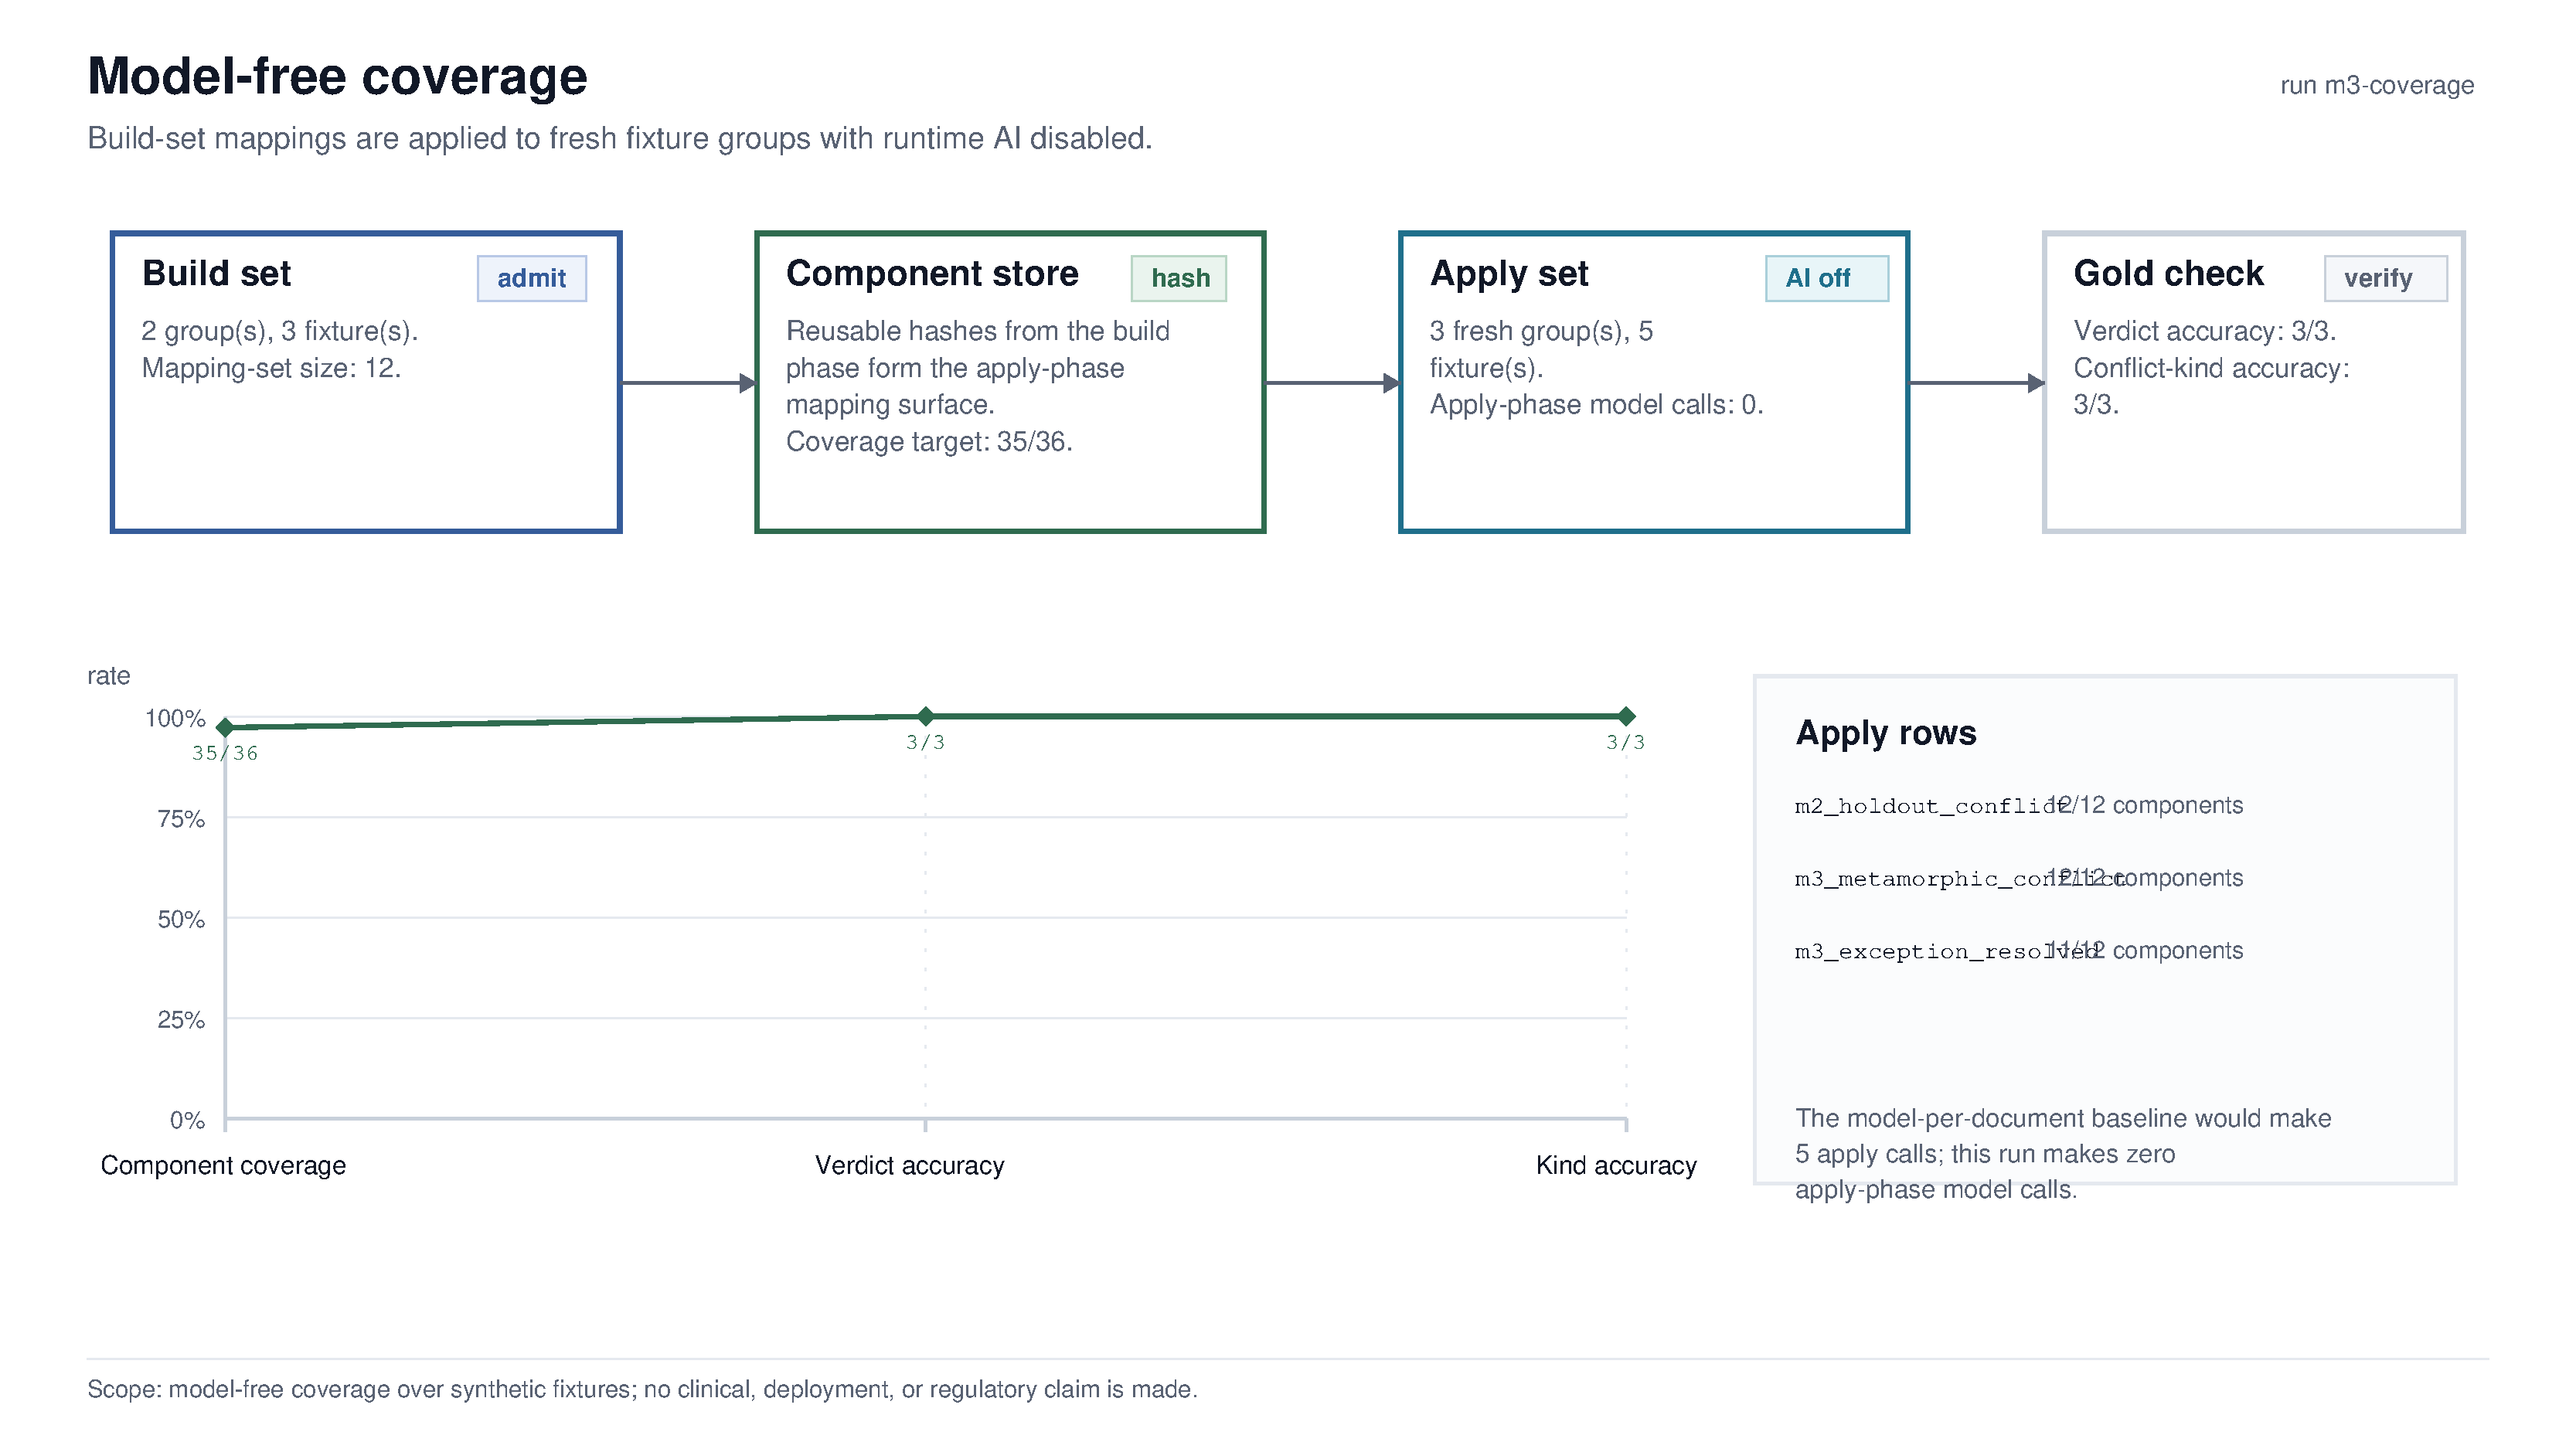
\includegraphics[width=\linewidth]{figures/manuscript/fig06_model_free_coverage.pdf}
  \caption{Model-free coverage. Build-set mappings are applied to fresh synthetic fixture groups with runtime AI disabled; component coverage, verdict accuracy, and zero apply-phase model calls are reported as exact ratios/counts.}
  \label{fig:model-free-coverage}
\end{figure}
